\documentclass[11pt,a4paper]{article}
\usepackage[top=3cm, bottom=2cm, left=2cm, right=2cm]{geometry}
\usepackage[utf8]{inputenc}
\usepackage{amsmath, amsfonts, amssymb}
\usepackage{siunitx}
\usepackage[brazil]{babel}
\usepackage{graphicx}
\usepackage[margin=10pt,font={small, it},labelfont=bf, textfont=it]{caption}
\usepackage[dvipsnames, svgnames]{xcolor}
\DeclareCaptionFont{MediumOrchid}{\color[svgnames]{MediumOrchid}}
\usepackage[pdftex]{hyperref}
\usepackage{natbib}
\bibliographystyle{plainnat}
\bibpunct{\textcolor{MediumOrchid}{\textbf{[}}}{\textcolor{MediumOrchid}{\textbf{]}}}{,}{s}{}{}
\usepackage{color}
\usepackage{footnote}
\usepackage{setspace}
\usepackage{booktabs}
\usepackage{multirow}
\usepackage{subfigure}
\usepackage{fancyhdr}
\usepackage{leading}
\usepackage{indentfirst}
\usepackage{wrapfig}
\usepackage{mdframed}
\usepackage{etoolbox}
\usepackage[version=4]{mhchem}
\usepackage{enumitem}
\usepackage{caption}
\usepackage{titlesec}
\usepackage{tcolorbox}
\usepackage{tikz}
\usepackage{LobsterTwo}
\usepackage[T1]{fontenc}
\usepackage{fontspec}
\usepackage{txfonts}
\usepackage[bottom]{footmisc}
\tcbuselibrary{skins,breakable}
\sisetup{output-decimal-marker={.}}

\makeatletter
\def\footnoterule{\kern-3pt\color{MediumOrchid}\hrule\@width0.6\textwidth height 0.8pt\kern2.6pt}
\makeatother

\renewcommand{\footnotelayout}{\itshape\color{MediumOrchid}}

\AtBeginEnvironment{equation}{\fontsize{13}{16}\selectfont}


\titleformat{\section}{\LobsterTwo\huge\color{CarnationPink}}{\thesection.}{1em}{}
\titleformat{\subsection}{\LobsterTwo\huge\color{CarnationPink}}{\thesubsection}{1em}{}
\titleformat{\subsubsection}{\bf\LobsterTwo\Large\color{MediumOrchid}}{\thesubsubsection}{1em}{}


\DeclareCaptionLabelFormat{figuras}{\textcolor{DarkTurquoise}{Figura \arabic{figure}}}
\captionsetup[figure]{labelformat=figuras}

\makeatletter
\renewcommand\tagform@[1]{\maketag@@@{\color{CarnationPink}(#1)}}
\makeatother

\renewcommand{\theequation}{Eq. \arabic{equation}}
\renewcommand{\thefigure}{Fig. \arabic{figure}}
\renewcommand{\thesection}{\textcolor{CarnationPink}{\arabic{section}}}

\setlist[itemize]{label=\textcolor{CarnationPink}{$\blacksquare$}}

\setlist[enumerate]{label=\textcolor{CarnationPink}{\arabic*.}, align=left, leftmargin=1.5cm}


\newcounter{exemplo}

\NewDocumentEnvironment{exemplo}{ O{} }{%
\allowbreak
\setlength{\parindent}{0pt}
  \begin{mdframed}[
  leftline=true,
  topline=false,
  rightline=false,
  bottomline=false,
  linewidth=2pt,
  linecolor=CarnationPink,
  frametitlerule=false,
  frametitlefont=\LobsterTwo\large\color{CarnationPink},
  frametitle={\color{CarnationPink}\LobsterTwo\large #1},
  ]
}{%
  \end{mdframed}
}

\setlength{\fboxsep}{5pt}
\setlength{\fboxrule}{1.5pt}
\usepackage{float}
\renewcommand{\thefootnote}{\alph{footnote}}
\usepackage{url}
\hypersetup{
	colorlinks=true,
	linkcolor=DarkTurquoise,
	filecolor=DarkTurquoise,      
	urlcolor=DarkTurquoise,
	citecolor=DarkTurquoise,
	pdftitle={Especialista em Física da Radioterapia}
}
\pagestyle{fancy}
\fancyhf{}
\renewcommand{\headrulewidth}{0pt}
\rfoot{\color{DarkTurquoise}\thepage \\ \LobsterTwo{\textcolor{CarnationPink}{@defDalila}}}


\title{\LobsterTwo\Huge{Dosimetria}}
\author{\LobsterTwo\Large{Detectores de Radiação\nocite{*}}}
\date{\LobsterTwo\textit{Dalila Mendonça}}
\begin{document}
	\maketitle

\section{Características dos Detectores}

\subsection*{Precisão e Exatidão}

	Na dosimetria em radioterapia, é essencial considerar a incerteza associada às medições realizadas. Essa incerteza é geralmente expressa em termos de exatidão e precisão. A \textcolor{MediumOrchid}{\textit{\textbf{precisão}}} refere-se à \textcolor{MediumOrchid}{\textit{\textbf{capacidade de reproduzir resultados semelhantes em medições repetidas sob condições semelhantes}}}. Uma alta precisão é indicada por um pequeno desvio padrão na distribuição dos resultados de medição, o que implica em uma boa reprodutibilidade dos valores obtidos.

	Já a \textcolor{MediumOrchid}{\textit{\textbf{exatidão}}} está relacionada à \textcolor{MediumOrchid}{\textit{\textbf{proximidade entre o valor medido e o valor verdadeiro}}} da grandeza em questão. Em medições dosimétricas, a exatidão é avaliada comparando-se os resultados obtidos com um valor de referência conhecido ou aceito como verdadeiro. É importante ressaltar que é difícil obter medições completamente exatas, e qualquer falta de exatidão é considerada como incerteza.

	A \textcolor{MediumOrchid}{\textit{\textbf{incerteza}}} é um parâmetro que descreve a \textcolor{MediumOrchid}{\textit{\textbf{dispersão dos valores medidos para uma grandeza}}}. Geralmente, é avaliada utilizando-se \textcolor{MediumOrchid}{\textit{\textbf{métodos estatísticos}}} (conhecidos como Tipo A) ou \textcolor{MediumOrchid}{\textit{\textbf{outras abordagens}}} (conhecidas como Tipo B). A incerteza é assumida como não tendo um sinal conhecido e é frequentemente considerada simétrica. A quantificação da incerteza permite uma estimativa do intervalo no qual o valor verdadeiro provavelmente está contido.

	Por outro lado, o \textcolor{MediumOrchid}{\textit{\textbf{erro}}} de medição é definido como a \textcolor{MediumOrchid}{\textit{\textbf{diferença entre o valor medido de uma grandeza e o seu valor verdadeiro}}}. Os erros têm um valor numérico e um sinal associado. Embora seja difícil conhecer precisamente os erros de medição, eles são estimados da melhor maneira possível e correções compensatórias são aplicadas sempre que possível.

	Após aplicar todas as correções conhecidas, idealmente, espera-se que o valor médio dos erros seja zero. No entanto, a preocupação principal passa a ser a quantificação das incertezas associadas às medições. Essa quantificação permite que se tenha uma ideia clara da dispersão dos resultados e ajuda a avaliar a confiabilidade das medições realizadas.

\subsection*{Linearidade}

	Idealmente, a leitura M dosímetro deve apresentar uma proporção linear com a quantidade dosimétrica Q. Isso significa que a \textcolor{MediumOrchid}{\textit{\textbf{leitura do dosímetro deve ser diretamente proporcional à quantidade de radiação recebida}}}, de modo que \textcolor{MediumOrchid}{\textit{\textbf{um aumento na dose resulte em um aumento proporcional na leitura do dosímetro}}}. No entanto, além de uma determinada faixa de dose, uma resposta não linear é observada. Isso significa que a relação entre a dose e a leitura do dosímetro deixa de ser estritamente proporcional. O comportamento não linear pode surgir devido a diversas razões, como interações complexas entre a radiação e o material do dosímetro, efeitos de saturação ou outros fenômenos físicos específicos do tipo de dosímetro utilizado.

	A \ref{fig:linearidade} ilustra dois exemplos típicos de características de resposta observadas em sistemas de dosimetria. A \textcolor{DarkTurquoise}{\textit{\textbf{Curva A}}} representa um dosímetro que inicialmente apresenta uma relação linear entre a dose e a leitura do dosímetro. No entanto, à medida que a dose aumenta, ocorre um comportamento \textcolor{MediumOrchid}{\textit{\textbf{supralinear}}}, ou seja, \textcolor{MediumOrchid}{\textit{\textbf{a resposta do dosímetro aumenta em uma taxa maior do que o esperado}}} pela linearidade. Eventualmente, a curva atinge um ponto de saturação, onde a leitura do dosímetro não aumenta mais, mesmo que a dose continue aumentando. Por outro lado, a \textcolor{DarkTurquoise}{\textit{\textbf{Curva B}}} também apresenta linearidade inicial, mas atinge a \textcolor{MediumOrchid}{\textit{\textbf{saturação}}} em doses mais elevadas, ou seja, \textcolor{MediumOrchid}{\textit{\textbf{a leitura do dosímetro não aumenta além de um determinado limite, mesmo com o aumento da dose}}}.

	\begin{figure}[h]
		\centering
		\fcolorbox{DarkTurquoise}{white}{%
			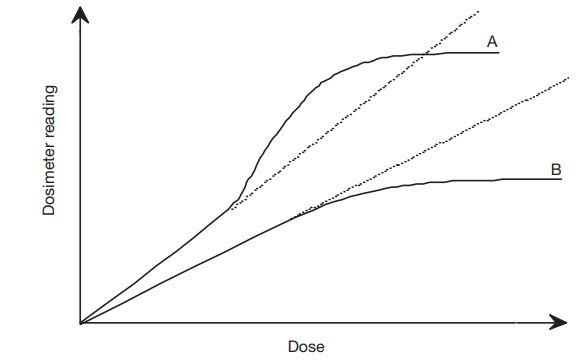
\includegraphics[width=0.5\textwidth]{Imagens/linearidade.JPG}
		}%
		\caption{As características de resposta de dois sistemas de dosimetria são as seguintes: Curva A: Inicialmente, demonstra linearidade com a dose, seguida por uma transição para um comportamento supralinear e, eventualmente, atinge a saturação. Curva B: Inicialmente, exibe linearidade com a dose e, em seguida, atinge a saturação em doses elevadas..}
		\label{fig:linearidade}
	\end{figure}

	Em geral, é importante abordar o comportamento não linear.  Embora tanto o dosímetro quanto o seu leitor possam exibir características não lineares individualmente, é possível que o efeito combinado deles resulte em uma faixa mais ampla de linearidade. Isso significa que, mesmo que um dosímetro ou um leitor individualmente apresente não linearidade em certas faixas de dose, a combinação dos dois elementos pode compensar essas não linearidades e fornecer uma relação aproximadamente linear entre a dose e a leitura em uma faixa mais ampla de valores.

\subsection*{Dependência com a Taxa de Dose}

	Os sistemas de dosimetria integrados são projetados para medir a resposta cumulativa de um sistema de dosimetria. Esses sistemas são projetados para quantificar a quantidade total de radiação recebida ao longo do tempo, fornecendo uma medida integrada da exposição. Nesses sistemas, é desejável que \textcolor{MediumOrchid}{\textit{\textbf{a quantidade dosimétrica medida não seja afetada pela taxa na qual a radiação é entregue}}}. Em outras palavras, a resposta do sistema de dosimetria, representada pela razão $M/Q$(onde M é a leitura do dosímetro e Q é a quantidade dosimétrica medida), idealmente deve permanecer \textcolor{MediumOrchid}{\textit{\textbf{constante}}} mesmo quando a taxa de dose é alterada. Isso significa que a leitura do dosímetro deve ser independente da taxa de dose aplicada.

	No entanto, na prática, \textcolor{MediumOrchid}{\textit{\textbf{a taxa de dose pode afetar as leituras do dosímetro}}} e, portanto, correções adequadas são necessárias. Isso ocorre porque certos \textcolor{MediumOrchid}{\textit{\textbf{efeitos físicos}}} podem estar relacionados à \textcolor{MediumOrchid}{\textit{\textbf{taxa de dose}}} e podem influenciar a resposta do dosímetro. Por exemplo, em feixes pulsados, onde a radiação é entregue em pulsos intermitentes, as câmaras de ionização utilizadas como dosímetros podem apresentar um fenômeno conhecido como \textcolor{MediumOrchid}{\textit{\textbf{recombinação iônica}}}. A recombinação iônica ocorre quando a \textcolor{MediumOrchid}{\textit{\textbf{taxa de dose é alta o suficiente para que as cargas elétricas geradas pela radiação não tenham tempo suficiente para se separarem completamente}}} antes do próximo pulso de radiação. Esse efeito pode levar a uma subestimação da leitura do dosímetro, exigindo correções específicas para levar em consideração a influência da taxa de dose.

\subsection*{Dependência Energética}

	A resposta de um sistema de dosimetria, representada pela razão $M/Q$, é geralmente influenciada pela qualidade (energia) do feixe de radiação. Isso significa que a \textcolor{MediumOrchid}{\textit{\textbf{resposta do dosímetro}}}, medida pela leitura M, \textcolor{MediumOrchid}{\textit{\textbf{pode variar dependendo da energia do feixe de radiação utilizado}}}. Os sistemas de dosimetria são normalmente calibrados usando qualidades específicas de feixes de radiação, mas na prática frequentemente são utilizados em uma faixa mais ampla de energias. Essa variação na resposta do dosímetro com a energia do feixe de radiação é conhecida como \textcolor{MediumOrchid}{\textit{\textbf{dependência energética}}} e requer correção para garantir medidas precisas.

	Idealmente, a resposta de energia de um sistema de dosimetria deve ser consistente, o que significa que a calibração do sistema deve ser independente da energia dentro de uma faixa específica de qualidades de radiação. No entanto, na realidade, é comum que uma correção para a qualidade de energia precise ser aplicada ao determinar a quantidade dosimétrica Q na maioria das situações de medição. Isso ocorre porque nenhum dosímetro consegue reproduzir perfeitamente as propriedades da água ou do tecido em todas as qualidades de feixes de radiação. Portanto, a dependência energética se torna uma característica significativa de um sistema de dosimetria.

	No contexto da radioterapia, a quantidade dosimétrica desejada é a dose para a água ou tecido. Entretanto, como mencionado anteriormente, nenhum dosímetro é capaz de replicar completamente as propriedades da água ou do tecido em todas as energias do feixe de radiação. Consequentemente, a dependência energética se torna uma consideração importante ao medir a dose em radioterapia. A correção de energia é necessária para compensar as diferenças na resposta do dosímetro em relação à energia do feixe de radiação, garantindo uma medida correta da quantidade dosimétrica Q, ou seja, a dose absorvida.

\subsection*{Dependência Direcional}

	A \textcolor{MediumOrchid}{\textit{\textbf{variação na resposta de um dosímetro com base no ângulo de incidência da radiação}}} é chamada de dependência direcional ou dependência angular. Isso significa que a leitura do dosímetro pode ser afetada pela direção ou ângulo sob o qual a radiação incide sobre ele. Essa dependência direcional é uma propriedade dos dosímetros e pode ocorrer devido a diversos fatores, como suas características construtivas (geométricas), dimensões físicas e a energia da radiação incidente.

	Os dosímetros frequentemente apresentam dependência direcional devido a esses fatores mencionados anteriormente. As \textcolor{MediumOrchid}{\textit{\textbf{características construtivas do dosímetro}}}, como a geometria e a composição do material sensível à radiação, podem influenciar sua resposta em diferentes ângulos de incidência. Além disso, as \textcolor{MediumOrchid}{\textit{\textbf{dimensões físicas do dosímetro}}}, como o tamanho e a espessura dos detectores, também podem desempenhar um papel importante na dependência direcional. A \textcolor{MediumOrchid}{\textit{\textbf{energia da radiação incidente}}} também pode influenciar a resposta do dosímetro em diferentes ângulos.

	Essa característica de dependência direcional é particularmente significativa em aplicações específicas, como dosimetria in vivo, onde dosímetros semicondutores são utilizados. Nesses casos, a dependência direcional pode afetar a precisão das medidas quando o dosímetro é exposto a diferentes ângulos de incidência da radiação dentro do paciente. Portanto, é importante levar em consideração essa dependência direcional ao utilizar dosímetros semicondutores em dosimetria in vivo.

	Os dosímetros clínicos, geralmente utilizados para medir a dose em radioterapia, são tipicamente utilizados na mesma configuração geométrica em que foram calibrados. Isso significa que, durante o uso clínico, é levada em consideração a dependência direcional específica do dosímetro, considerando a geometria de irradiação que foi utilizada para a calibração do dosímetro. Essa abordagem garante que as medidas de dose sejam corrigidas para qualquer dependência direcional do dosímetro, garantindo assim a precisão adequada nas aplicações terapêuticas.

\subsection*{Resolução Espacial}


	A dose é uma \textcolor{MediumOrchid}{\textit{\textbf{quantidade localizada}}}, o que significa que é necessário que um \textcolor{MediumOrchid}{\textit{\textbf{dosímetro seja capaz de determinar a dose em um volume muito pequeno}}}. Em outras palavras, é necessário um "dosímetro pontual" que possa caracterizar a dose em um ponto específico. Além disso, a localização espacial desse ponto onde a dose é determinada deve ser precisamente definida dentro de um sistema de coordenadas de referência. Isso é importante para garantir medidas precisas e localizadas da dose em um determinado local.

	Os dosímetros termoluminescentes (TLDs) estão disponíveis em dimensões compactas, o que lhes permite se aproximar de medições pontuais. Eles podem ser usados para fornecer uma medida pontual precisa da dose em um ponto específico. Os filmes dosimétricos oferecem excelente resolução bidimensional, permitindo a caracterização da dose em duas dimensões. Esses dosímetros são frequentemente usados para medir a distribuição de dose em planos bidimensionais, como em teleterapia. Por fim, os dosímetros de gel fornecem resolução tridimensional, permitindo a medição precisa da dose em três dimensões. Esses dosímetros são usados em aplicações onde é necessário descrever a distribuição tridimensional da dose, como em braquiterapia. A capacidade de medição pontual com dosímetros de gel é limitada apenas pela capacidade de resolução do sistema de avaliação utilizado.

	Os dosímetros do tipo câmara de ionização possuem um tamanho finito para alcançar a sensibilidade necessária (efeito de média de volume). Isso ocorre porque as câmaras de ionização são projetadas para coletar cargas elétricas geradas pela radiação, e o tamanho e a geometria da câmara afetam sua sensibilidade. No entanto, é importante observar que o surgimento de microcâmaras pinpoint tem parcialmente abordado essa limitação de tamanho. As microcâmaras pinpoint são projetadas com dimensões menores, permitindo uma maior resolução espacial em comparação com as câmaras de ionização convencionais. Essas microcâmaras têm se mostrado úteis em aplicações que exigem alta resolução espacial, como a dosimetria em feixes estreitos ou tratamentos de radiocirurgia.

\subsection*{Facilidade de Leitura}

	Os dosímetros de leitura direta, como as câmaras de ionização, geralmente são considerados mais convenientes em comparação com os dosímetros passivos que requerem processamento pós-exposição antes da leitura, como os TLDs (dosímetros termoluminescentes) e filmes. Isso significa que os dosímetros de leitura direta permitem a obtenção imediata da leitura do dosímetro após a exposição à radiação, enquanto os dosímetros passivos exigem uma etapa adicional de processamento antes que os resultados possam ser obtidos.

	Certos dosímetros operam inerentemente como sistemas integrados, como os TLDs e géis. Isso significa que esses dosímetros são projetados para medir a dose cumulativa ao longo do tempo de exposição. Os TLDs, por exemplo, acumulam a energia da radiação durante a exposição e, em seguida, essa energia é liberada como luz quando o dosímetro é aquecido. Da mesma forma, os géis são capazes de registrar a distribuição tridimensional da dose ao longo do tempo. Esses dosímetros passivos são adequados para aplicações em que é necessário obter a dose total recebida.
	
	
\section{Propriedades Gerais dos Detectores de Radiação}

    Um detector quando submetido à radiação, terá um volume que será responsável por detectar a radiação e efetuar a leitura. Quando a radiação interage com o volume do detector, ela irá causar ionizações, ou seja, arrancará um elétron do átomo inicialmente neutro, e fará com que seja formado um par elétron íon, cargas negativas e cargas positivas. A interação ou o total freamento da partícula ocorre em um tempo muito curto, o que permite dizer que a deposição de energia é feita instantaneamente. 

    Assumindo a interação devido a apenas um quanta de energia (uma única partícula), a carga gerada dentro do detector ocorrerá então no tempo $t = 0$ (instantâneo). Na sequência, a carga deverá ser coletada na forma de sinais elétricos, cujo processo de detecção normalmente está acompanhado de um campo elétrico interno, que faz com que as cargas positivas e negativas se movam em direções opostas. 

    O tempo para coletar todas as cargas formadas nos detectores varia de um tipo de detector para outro, por exemplo as câmaras de ionização o tempo para coletar todas as cargas é da ordem de poucos milissegundos, enquanto que o tempo de coleção dos  diodos semicondutores é da ordem de poucos nanossegundos. Esses tempos de coleta estão relacionados à mobilidade dos portadores de carga e também à distância que os portadores de carga percorrem até serem coletadas no eletrodo coletor.

    Portanto, para a interação de apenas um quanta de energia, a resposta do detector será uma corrente que flui por um tempo igual ao tempo de coleta da carga. A  \ref{fig:esquemaTempoColetaCorrente} mostra uma possível dependência temporal da corrente do detector, onde $t_c$ é o tempo para coletar a carga;

        \begin{figure}[h]
            \centering
            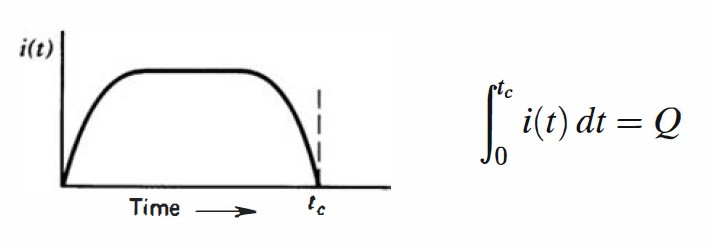
\includegraphics[width=0.7\textwidth]{Imagens/esquemaTempoColetaCorrente.jpg}
            \caption{Corrente em função do tempo de coleta da carga}
            \label{fig:esquemaTempoColetaCorrente}
        \end{figure}

	\noindent A integral da corrente ao longo de todo o tempo de coleta é igual quantidade total de carga gerada naquela interação específica. 

	Em situações reais, vários quantas estão interagindo com o volume do detector ao longo de um período de tempo. Portanto, para os casos em que há uma alta taxa de irradiação, a corrente gerada pode ser devida a mais de uma interação.  Assumindo que o detector está submetido a uma baixa taxa de radiação, de forma que cada interação irá gerar uma corrente que pode ser distinguida das demais interações. A medida que cada interação ocorre, serão gerados pulsos de correntes elétricas de modo que a intensidade de duração do pulso de corrente poderá variar dependendo do tipo de interação. A  \ref{fig:esquemaCorrentePulsada} mostra um esquema da corrente elétrica instantânea fluindo no detector ao longo do tempo.

		\begin{figure}[h]
			\centering
			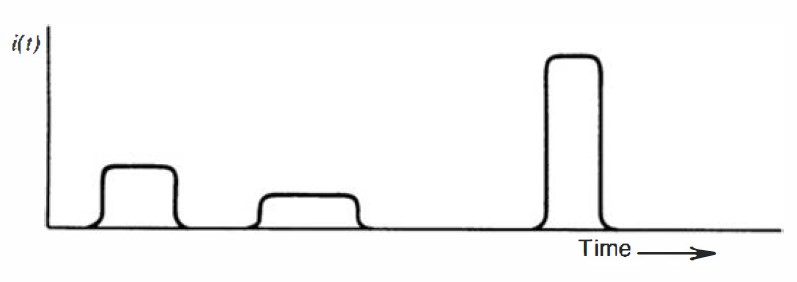
\includegraphics[width=0.7\textwidth]{Imagens/esquemaCorrentePulsada.jpg}
			\caption{Esquema de Pulsos de Corrente ao longo do tempo de medição do detector}
			\label{fig:esquemaCorrentePulsada}
		\end{figure}

	\noindent Pode-se observar diferentes intensidades de corrente e diferentes tempos de coleta de cada pulso. Nota-se também que, como a emissão de radiação é um processo aleatório, os intervalos de tempo entre um pulso de corrente e outro também é aleatoriamente distribuído. 
      
	\subsection*{Modos de Operação Dos Detectores}

		Existem três modos de operação dos detectores, \textcolor{MediumOrchid}{\textbf{\textit{Modo Pulso, Modo Corrente e Modo de tensão quadrada média (MSV)}}}; ambos operam de forma diferente e estão inter-relacionados através de suas dependências com as sequências de pulsos de correntes geradas no detector. 

		Como a energia depositada no detector é diretamente relacionada com a carga total $Q$ geradas através das interações dos quantas de energia com o detector, é de interesse que todas as cargas sejam coletadas e portanto o instrumento de medição irá operar no \textcolor{MediumOrchid}{\textit{\textbf{modo pulso}}} de forma que toda interação individual seja registrada. 

		O \textcolor{MediumOrchid}{\textit{\textbf{modo pulso}}} também é utilizado nos \textcolor{MediumOrchid}{\textit{\textbf{contadores de pulsos}}}, que se enquadra naquelas situações \textcolor{MediumOrchid}{\textit{\textbf{onde não é de interesse registrar a distribuição de energia da radiação}}}, ou seja, não é de interesse obter energia depositada pelos quantas de radiação, o interesse é apenas \textcolor{MediumOrchid}{\textit{\textbf{obter a intensidade da radiação incidente}}}; Para estes casos, é estabelecido um limiar de baixo nível para os pulsos gerados de forma qua qualquer pulso de corrente acima deste limiar é registrado pelo detector, independente do valor de Q.

		O \textcolor{MediumOrchid}{\textit{\textbf{modo corrente}}} e o \textcolor{MediumOrchid}{modo MSV} são utilizados naquelas situações em que a \textcolor{MediumOrchid}{\textit{\textbf{taxa radiação é muito alta}}} de forma que o modo pulso seja impraticável pois o \textcolor{MediumOrchid}{\textit{\textbf{tempo entre eventos adjacentes é muito pequeno}}} de forma que não seja possível realizar uma análise adequada da carga coletada e os pulsos de corrente gerados podem se sobrepor ao longo do tempo; Sendo necessário, então, utilizar instrumentos de medição que respondem à media de tempo no qual ocorrem muitos eventos individuais;

		\subsubsection*{Modo Corrente}

			A  \ref{fig:esquemaModoCorrente} apresenta o esquema de um detector operando no modo corrente, onde um amperímetro é conectado aos terminais de saída do detector de radiação;

				\begin{figure}[h]
					\centering
					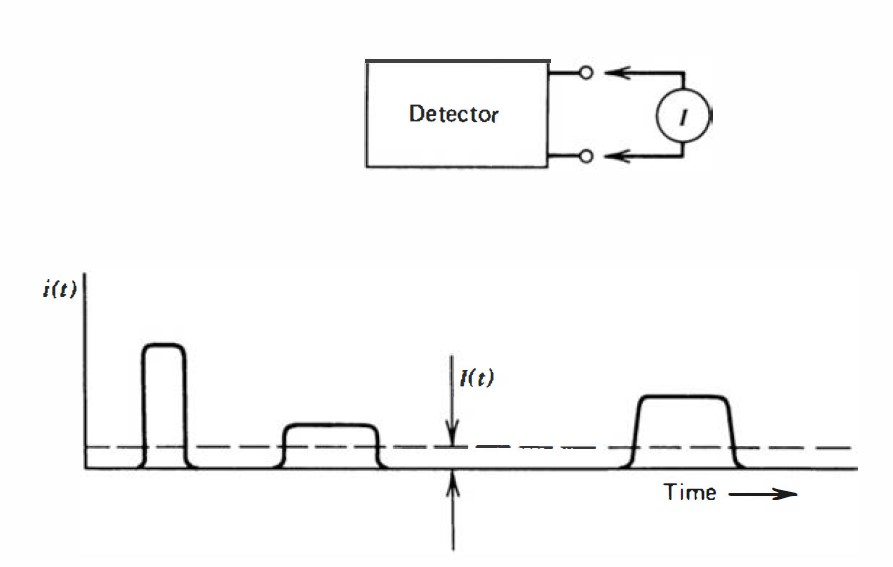
\includegraphics[width=0.7\textwidth]{Imagens/esquemaModoCorrente.jpg}
					\caption{Esquema de Detector Operando no Modo Corrente.}
					\label{fig:esquemaModoCorrente}
				\end{figure}
			
			No modo corrente, assume-se que o \textcolor{MediumOrchid}{\textit{\textbf{tempo de resposta T do detector é fixo}}}, e portando diversos pulsos de corrente emitidos em um tempo t serão coletados ao longo do tempo de resposta do detector, gerando uma corrente dependente do tempo dada por:
			
				\begin{equation}
					I(t) = \frac{1}{T} \int_{t-T}^{t} i (t') \,dt' 
				\end{equation}

			\noindent Como o tempo de resposta T é muito maior que o intervalo de tempo entre os pulsos de corrente individuais, o efeito é compensar muitas das flutuações nos intervalos entre as interações individuais e registrar uma corrente média que depende do produto da taxa de interação e a carga média por interação.

			A corrente média é dada pelo produto da taxa de eventos com a média de carga produzida por cada evento; portanto:

				\begin{equation}
					I_0 = rQ = r\frac{E}{W}q
				\end{equation}
			
			\begin{exemplo}[onde:]
				\begin{itemize}
					\item \textcolor{DarkTurquoise}{$\mathbf{r}$} é a Taxa de Eventos
					\item \textcolor{DarkTurquoise}{$\mathbf{Q}$} é a carga produzida por cada evento
					\item \textcolor{DarkTurquoise}{$\mathbf{E}$} é a energia média depositada por cada evento
					\item \textcolor{DarkTurquoise}{$\mathbf{W}$} é a Energia média para produzir um par elétron-íon
					\item \textcolor{DarkTurquoise}{$\mathbf{q}$} é a carga elétrica ($1.6 \times 10^{-19}C$)
				\end{itemize}
			\end{exemplo}


			Para uma irradiação estacionária do detector, a corrente média pode ser descrita como a soma da corrente constante $I_0$ com a componente de flutuação da corrente dependente do tempo ($\sigma_i(t)$), no qual é a variável aleatória dependente do tempo que ocorre como consequência da natureza aleatória dos eventos interagindo com o detector,  como mostra a  \ref{fig:esquemaCorrenteFlutuacao}.

			\begin{figure}[h]
				\centering
				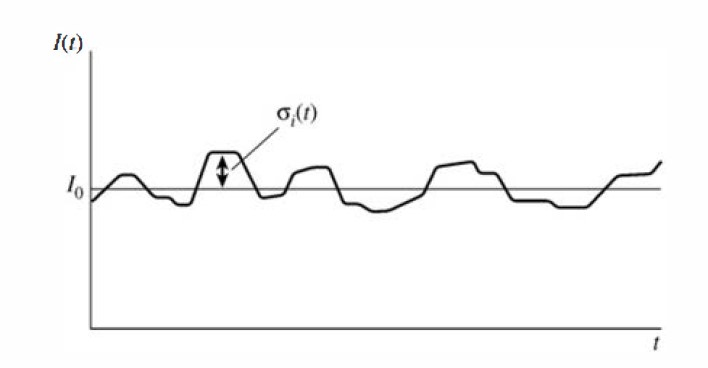
\includegraphics[width=0.7\textwidth]{Imagens/esquemaCorrenteFlutuação.jpg}
				\caption{Irradiação estacionária com flutuação}
				\label{fig:esquemaCorrenteFlutuacao}
			\end{figure}

		\subsubsection*{Modo Pulso}

			A natureza do sinal produzido por um único evento depende das características de entrada do circuito no qual o detector está conectado, normalmente utilizando um pré-amplificador. A  \ref{fig:esquemaModoPulso} apresenta um esquema básico de um circuito utilizado no modo pulso. 

				\begin{figure}[h]
					\centering
					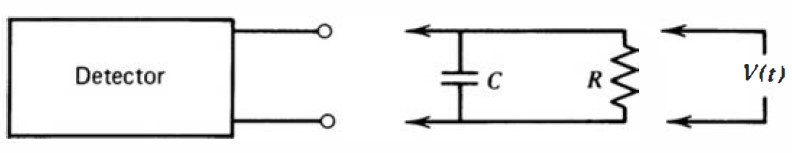
\includegraphics[width=0.8\textwidth]{Imagens/esquemaModoPulso.jpg}
					\caption{Circuitos de um detector operando em modo pulso}
					\label{fig:esquemaModoPulso}
				\end{figure}

				\begin{exemplo}[onde,]
					\begin{itemize}
						\item \textcolor{DarkTurquoise}{$\mathbf{R}$} representa a resistência de entrada do circuito;
						\item \textcolor{DarkTurquoise}{$\mathbf{C}$} representa a capacitância equivalente que considera a capacitância do detector e do circuito de medição; 
						\item \textcolor{DarkTurquoise}{$\mathbf{V(t)}$} é a tensão dependente do tempo, com o qual o modo pulso é baseado.
					\end{itemize}
				\end{exemplo}

			Caso um pré-amplificador seja acoplado ao detector, então R será a resistência de entrada e C será a soma das capacitâncias do detector, do cabo que conecta o detector ao pré-amplificador e capacitância de entrada do próprio pré-amplificador.

			Resistência elétrica é a oposição que um material apresenta à passagem de corrente elétrica através dele. Essa oposição é causada pelos elétrons que compõem o material e que se movem em resposta a um campo elétrico aplicado, colidindo com outras partículas do material e transferindo energia para elas. 

			A resistência elétrica limita a quantidade de corrente elétrica que pode fluir através do circuito. A Lei de Ohm estabelece que a corrente elétrica que flui através de um material é diretamente proporcional à diferença de potencial elétrico aplicada (tensão) e inversamente proporcional à resistência elétrica do material, ou seja:

				\begin{equation}
					I = \frac{V}{R}
				\end{equation}

				\begin{exemplo}[onde,]
					\begin{itemize}
						\item \textcolor{DarkTurquoise}{$\mathbf{I}$} é a corrente elétrica dada em amperes (A);
						\item \textcolor{DarkTurquoise}{$\mathbf{V}$} é a diferença de potencial dada em volts (V); e
						\item \textcolor{DarkTurquoise}{$\mathbf{R}$}  é a resistência dada em ohms ($\Omega$).
					\end{itemize}
				\end{exemplo}


			A Capacitância é uma grandeza elétrica que mede a capacidade de um objeto de armazenar carga elétrica quando submetido a uma diferença de potencial elétrico e está envolvida em circuitos elétricos que possuem capacitores.
			
			Os capacitores são dispositivos eletrônicos que consistem em duas placas condutoras separadas por um material isolante (dielétrico). Quando uma tensão é aplicada ao capacitor, as cargas elétricas se acumulam nas placas, criando um campo elétrico entre elas. Esse campo elétrico é proporcional à carga elétrica armazenada no capacitor e inversamente proporcional à capacitância do capacitor.

			A capacitância é dada pela relação entre a carga elétrica armazenada e a diferença de potencial elétrico aplicada ao capacitor, dada por:

				\begin{equation}
					C = \frac{Q}{V}
				\end{equation}

				\begin{exemplo}[onde,]
					\begin{itemize}
						\item \textcolor{DarkTurquoise}{$\mathbf{C}$} é a capacitância em farads (F);
						\item \textcolor{DarkTurquoise}{$\mathbf{Q}$} é a carga elétrica armazenada em coulombs (C); e 
						\item \textcolor{DarkTurquoise}{$\mathbf{V}$} é a diferença de potencial elétrico (tensão) em volts (V) aplicada ao capacitor.
					\end{itemize}
				\end{exemplo}
			
			Um circuito RC é um circuito elétrico composto por um resistor (R) e um capacitor (C) conectados em série ou em paralelo. A operação desse circuito depende da capacidade do capacitor de armazenar e liberar carga elétrica.

			Quando uma tensão é aplicada ao circuito, o capacitor começa a carregar. Durante esse processo, a corrente elétrica flui através do resistor, reduzindo a tensão aplicada ao capacitor. A taxa de carga depende do valor da resistência e da capacitância do circuito, conforme determinado pela constante de tempo.

			A constante de tempo em um circuito RC é um parâmetro que indica a rapidez com que um capacitor carrega ou descarrega em resposta a uma mudança na tensão aplicada a ele através de um resistor. É uma medida do tempo necessário para que a tensão do capacitor atinja aproximadamente 63,2\% do seu valor final após uma mudança na tensão de entrada.

			Após um certo tempo, o capacitor atinge seu limite de carga máxima e começa a armazenar energia elétrica. Se a tensão aplicada ao circuito for interrompida, o capacitor começa a descarregar através do resistor, liberando a energia armazenada. A taxa de descarga também depende do valor da resistência e da capacitância, conforme determinado pela constante de tempo.
			
			A constante de tempo para um circuito RC  é dada por:
			
				\begin{equation}
					\tau = R \cdot C
				\end{equation}

				\begin{exemplo}[onde,]
					\begin{itemize}
						\item \textcolor{DarkTurquoise}{$\mathbf{\tau}$} é a constante de tempo em segundos;
						\item \textcolor{DarkTurquoise}{$\mathbf{R}$} é a resistência em ohms
						\item \textcolor{DarkTurquoise}{$\mathbf{C}$} é a capacitância em farads.
					\end{itemize}
				\end{exemplo}
			
			A constante de tempo é importante em circuitos que envolvem a carga e descarga de capacitores, pois ela afeta a taxa de mudança da tensão no capacitor e, portanto, o comportamento do circuito como um todo.
			
			Pode-se então avaliar dois extremos de operação: Quando a constante de tempo do circuito é muito menor que o tempo para a coleta da carga e quando a constante de tempo é muito maior que o tempo para a coleta da carga.

			\begin{wrapfigure}{r}{0.5\textwidth}
				\centering
				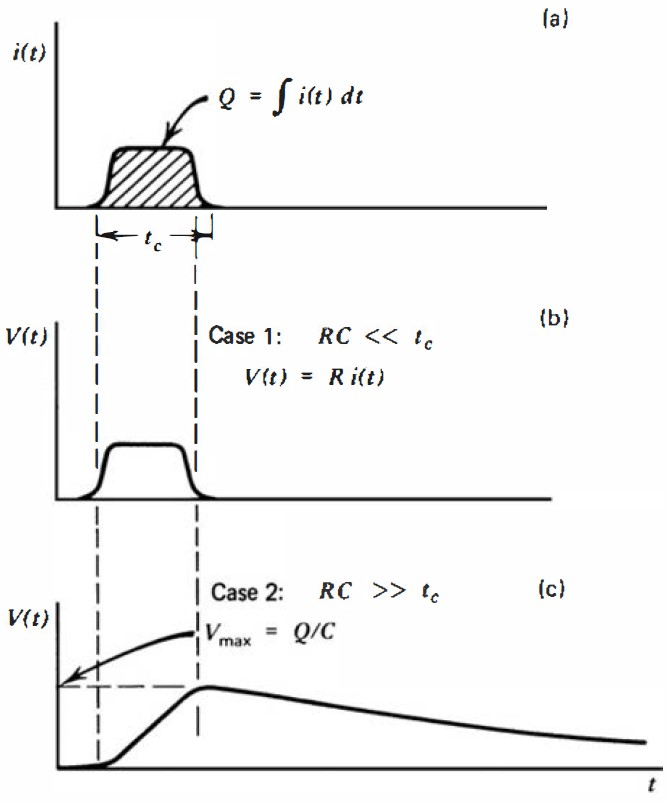
\includegraphics[width=0.41\textwidth]{Imagens/esquemaCorrentesCircuitoRC.jpg}
				\caption{Extremos de Operação}
				\label{fig:esquemaCorrenteCircuitoRC}
			\end{wrapfigure}


			$\tau \ll t_c$: Neste caso a constante de tempo do circuito externo é mantida pequena comparada ao tempo para coleta da carga, de forma que a corrente fluindo através da resistência R é essencialmente igual ao valor instantâneo da corrente fluindo no detector. O sinal da voltagem V(t) produzidos sob estas condições tem a forma aproximadamente idêntica à dependência temporal da corrente produzida dentro do detector, como mostra a  \ref{fig:esquemaCorrenteCircuitoRC}(b). Os detectores de radiação as vezes operam sob estas condições quando informações a respeito de altas taxas de eventos ou informações temporais são mais importantes que uma informação precisa da energia.

			$\tau \gg t_c$: Este é o principal modo de operação dos detectores que operam no modo pulso. Neste caso a constante de tempo é mantida grande o suficiente quando comparada ao tempo de coleta da carga de modo que uma corrente muito pequena irá fluir através da resistência R durante o tempo de coleta da carga e a corrente do detector é momentaneamente integrada à capacitância. Se assumirmos que o tempo entre os pulsos é suficientemente grande, o capacitor começará a descarregar através da resistência, retornando a voltagem da resistência para zero, como mostra a  \ref{fig:esquemaCorrenteCircuitoRC} (c).


			\begin{itemize}
				\item O tempo necessário para o pulso do sinal alcançar seu valor máximo é determinado pelo tempo de coleção de carga dentro do próprio detector;
				\item O tempo necessário para restaurar a tensão do sinal para zero é determinado apenas pela constante de tempo do circuito elétrico.
				\item A amplitude do pulso de sinal é determinada pela seguinte relação:
					\begin{equation}
						V_{max} = \frac{Q}{C}
					\end{equation}
			\end{itemize}

			Portanto, o output de um detector operando em modo pulso consiste em uma sequência de pulsos de sinais individuais representando o resultado da interação de uma única partícula com o detector, e a amplitude de cada pulso individual reflete a quantidade de carga liberada nessa interação.

			Só existe uma proporcionalidade entre $V_{max}$ e a Carga $Q$ caso a capacitância se mantenha constante. Na maior parte dos detectores, a capacitância inerente é dada pela a forma e tamanho do capacitor utilizado no circuito de forma que é garantida uma capacitância constante. Em outros casos, como ocorre com os diodos semi-condutores, a capacitância pode mudar devido a uma variação nos parâmetros normais de operação. Nestes casos, pulsos de voltagem com diferentes amplitudes podem ser gerados a partir da mesma carga total liberada na interação Q. 

			Comparando os detectores operando em modo pulso com os detectores operando em modo corrente, podemos inferir que:

			\begin{itemize}
				\item \textcolor{DarkTurquoise}{\textit{\textbf{A sensibilidade alcançada dos detectores operando no modo pulso é frequentemente muito maior que a sensibilidade dos detectores que operam no modo corrente}}}, pois cada interação individual pode ser detectada como um pulso distinto.
				\item No modo pulso, \textcolor{MediumOrchid}{\textit{\textbf{os limiares de detecção são definidos a partir dos níveis de radiação de fundo}}}; No modo corrente, a corrente mínima detectável pode representar uma taxa média de eventos muito maior que a radiação de fundo;
				\item No modo pulso, cara amplitude de pulso carrega alguma informação que é sempre útil ou uma parte necessária de uma aplicação em particular; Já no modo corrente, a informação a respeito da amplitude do pulso é perdida e todas as interações, independente da amplitude, contribuem para a corrente média medida. 
			\end{itemize}

	\subsection*{Espectro de Altura de Pulso}

		Quando um detector opera no modo pulso, cada amplitude de pulso gerada carrega informação a cerca da carga gerada em cada interação; Porém, ao avaliar diversos pulsos, nota-se que as amplitudes nem sempre são as mesmas e isto se deve à diferenças de energias das partículas incidentes ou até mesmo flutuações inerentes à resposta do detector em feixes monoenergéticos. 

		A distribuição de amplitude de pulso pode ser utilizada para deduzir informações a respeito da radiação incidente ou para obter informações a respeito da operação do próprio detector. Estas distribuições podem ser exibidas na forma integral ou diferencial.



		\subsubsection*{Distribuição Diferencial de Altura de Pulso}

			A  \ref{fig:distribuicaoDeAlturaDePulso} (a) fornece uma distribuição hipotética onde: a abscissa é a escala linear de amplitude de pulso que vai de zero até o maior valor de amplitude observado para a fonte, fornecida em volts (V); O eixo das ordenadas representa o número diferencial $dN$  de pulsos observados para uma amplitude dentro de um incremento diferencial de amplitude $dH$, dividido por esse incremento, ou seja $dN/dH$, fornecido em \unit{V^{-1}}.

			O número de pulsos cuja amplitude está entre dois valores pré-determinados $H_1$ e $H_2$ podem ser obtidos através da área da curva limitada por estas duas amplitudes, ou seja:

				\begin{equation}
					N_{H_1 \rightarrow  H_2} = \int_{H_1}^{H_2} \frac{dN}{dH}  \,dH 
				\end{equation}

				\begin{figure}[h]
					\centering
					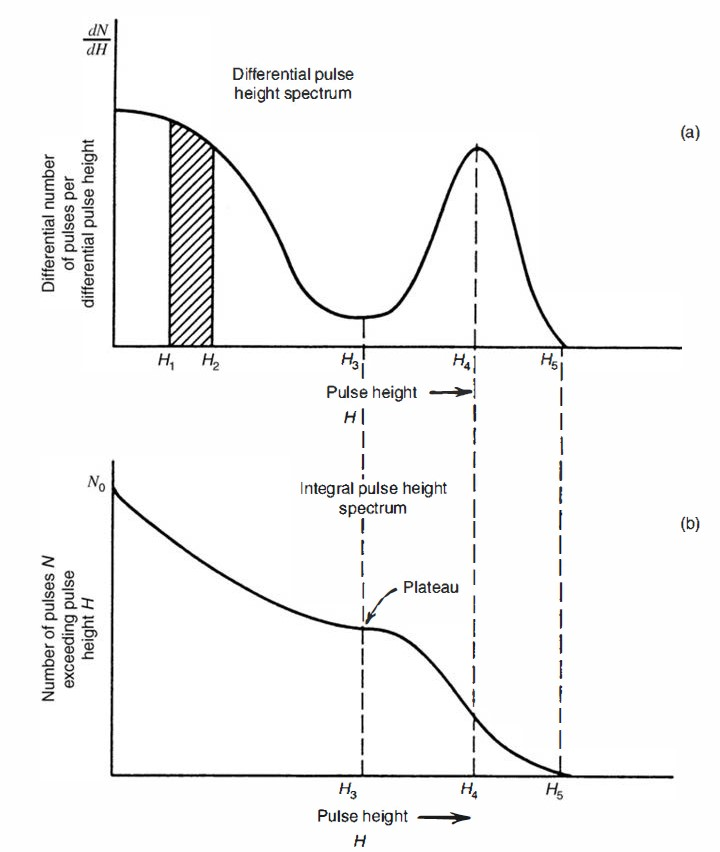
\includegraphics[width=0.59\textwidth]{Imagens/distribuicaoDeAlturaDePulso.jpg}
					\caption{Distribuições de Amplitude}
					\label{fig:distribuicaoDeAlturaDePulso}
				\end{figure}

			O número total de pulsos $N_0$ pode ser obtido através da área total embaixo da curva, ou seja:

				\begin{equation}
					N_0 = \int_{0}^{\infty} \frac{dN}{dH} \,dH
				\end{equation}

			A amplitude de pulso máxima observada ($H_5$) é o ponto ao longo da abscissa no qual a distribuição vai para zero; Picos na distribuição, como ocorre em $H_4$, indicam que são encontrados uma grande quantidade de pulsos para aquela amplitude de pulso; Os vales na distribuição, como ocorre em $H_3$, indicam que são encontrados poucos números de pulsos para aquela determinada amplitude de pulso. 

\subsubsection*{Distribuição Integral de Altura de Pulso}

	A  \ref{fig:distribuicaoDeAlturaDePulso} (b) mostra a distribuição integral para o mesmo espectro apresentado na  \ref{fig:distribuicaoDeAlturaDePulso} (a). O eixo das abscissas também representa a escala de amplitude de pulso, e o eixo das ordenadas apresenta o número de pulsos N no qual a amplitude excede o valor apresentado no eixo das abscissas H. N diminui em função H pois cada vez menos pulsos estarão acima de uma amplitude $H_i$ que pode aumentar seu valor além de zero. 
			
	Como todos os pulsos possuem uma amplitude finita maior que zero, então $H = 0$ representa o número total de pulsos observados $N_0$ e a medida que H aumenta a N diminui até que a distribuição integral cai para zero na amplitude de pulso máxima observada ($H_5$). 


	A amplitude da distribuição diferencial, ou seja, o número de pulsos de qualquer amplitude de pulso H é dada pelo valor absoluto da curva da distribuição integral no mesmo valor H; Nos locais onde aparecem picos na distribuição diferencial, representam pontos de máximo local na distribuição integra; E semelhantemente, as regiões de vale na distribuição diferencial representa os mínimos locais de amplitudes de pulsos na distribuição integral. 


\subsection*{Curvas de Contagem e Platôs}

	Quando os detectores operam no modo de contagem pulsada, os pulsos do detector são enviados para um dispositivo de contagem que possui um nível fixo de discriminação, ou seja possui um limiar de amplitude de pulso. Para que um pulso de sinal seja registrado pelo circuito do contador este pulso deverá exceder um limiar de amplitude de pulso $H_d$. É possível variar o limiar $H_d$ durante a medição afim de se obter informações a cerca da distribuição de amplitudes de pulso, e medidas realizadas com estas variações resultará da distribuição integral de amplitudes de pulso. 

	Ao realizar uma medida de contagem, a medição deverá ser conda de modo que se estabeleça um ponto de operação no qual irá ser alcançada a maior estabilidade sob longos períodos de tempo. Ou seja, durante uma medição podem ocorrer pequenos desvios em $H_d$ e portanto deve ser estabelecido um ponto de operação que fará com que esse desvio tenha influência mínima na contagem medida. Como mostra a  \ref{fig:distribuicaoDeAlturaDePulso}, o ponto em $H_3$ se con como um ponto estável de operação; Este ponto representa o ponto de mínimo global da distribuição diferencial de forma que representa um ponto com  variação mínima na curva integral, portanto pequenos desvios no limiar $H_d$ terão um impacto mínimo no número total de pulsos registrados. No geral, regiões de mínimo na curva integral são chamados de platô de contagem e representam áreas de operação no qual é possível alcançar uma sensibilidade mínima a variações no limiar de amplitude. 

	O platô em contagem de dados também é observado em processos no qual a carga produzida a cada interação é aumentada para um determinado detector de radiação; onde muitas vezes é possível variar o ganho ou a amplificação fornecida para a carga produzida na interação. Esta variação pode ser feita alterando o fator de amplificação de um amplificador linear posicionado entre o detector e o circuito de contagem, ou pode ser feita diretamente alterando a voltagem aplicada no próprio detector. 

	A  \ref{fig:curvaContagemGanho} (a) apresenta uma distribuição diferencial de amplitude de pulso, para três valores diferentes de ganho da voltagem. Neste caso, o valor do ganho (G) pode ser definido como a razão entre a amplitude da voltagem para um dado evento no detector e a mesma amplitude antes de algum parâmetro ser alterado, como o fator de amplificação ou a voltagem do detector. 

			\begin{figure}[h]
				\centering
				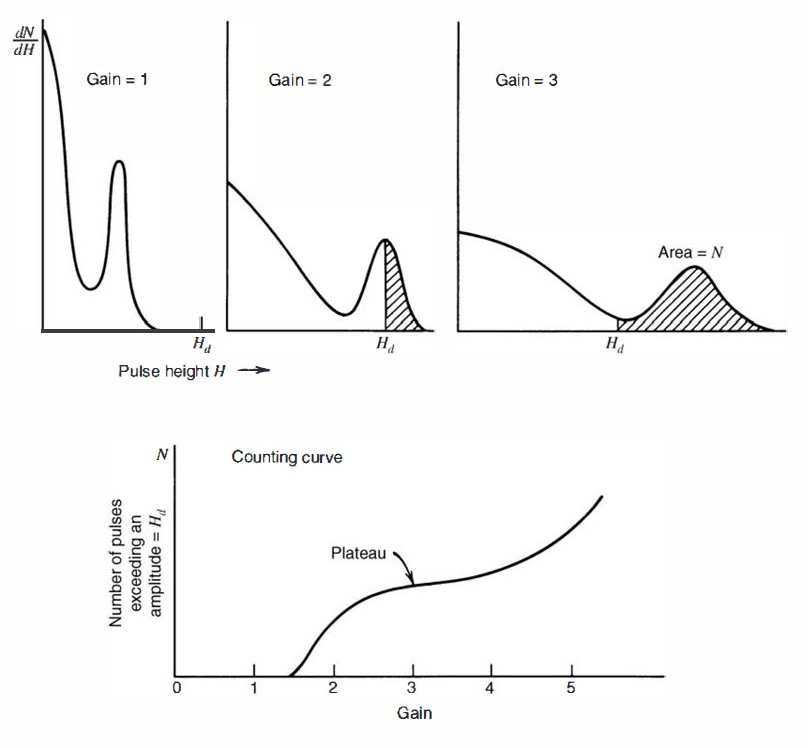
\includegraphics[width=0.8\textwidth]{Imagens/curvaContagemGanho.jpg}
				\caption{Exemplo de uma curva de contagem gerada através da variação do ganho mantendo as condições da fonte constante}
				\label{fig:curvaContagemGanho}
			\end{figure}

		
	Ao manter a irradiação constante, quanto maior o ganho na voltagem maior será a amplitude de pulso máxima, porém em ambos os casos a área sob a curva diferencial se manterá constante, ou seja, o número total de pulsos  será sempre o mesmo. A  \ref{fig:curvaContagemGanho} mostra que para o ganho G = 1, nenhuma contagem será registrada pois todas as amplitudes de pulso estão abaixo do limiar de amplitude para detecção. Ao realizar contagens em função do ganho da voltagem, obtem-se a distribuição integral, chamada de curva de contagens, apresentada na  \ref{fig:curvaContagemGanho} (b). Devido à pequenos valores de ganho, nenhum pulso é contado, porem a medida que o ganho é aumentado, aumenta-se o número de pulsos contados até que o ganho seja suficiente para contar todos os pulsos. 

	O platô na curva de contagem pode ser previsto com base no valor de ganho que faz com que o limiar de amplitude $H_d$ coincida aproximadamente com um ponto de mínimo na curva diferencial. 


\subsection*{Resolução de Energia}

	Diversas aplicações de detectores de radiação tem como objetivo medir a distribuição de energia da radiação incidente, chamado de forma geral como espectroscopia da radiação. A  \ref{fig:funcoesDeResposta} ilustra a distribuição diferencial de amplitude de pulso produzida por um detector submetido a um feixe monoenergético; Esta distribuição é chamada de \textcolor{MediumOrchid}{\textit{\textbf{função resposta}}} de um detector para a energia utilizada na sua determinação. A curva chamada de \textcolor{MediumOrchid}{\textit{\textbf{``Boa Resolução''}}} ilustra uma possível distribuição em torno da amplitude média de pulso $H_0$; A curva chamada de \textcolor{MediumOrchid}{\textit{\textbf{``Baixa Resolução''}}}, ilustra a resposta de um detector com um desempenho inferior. Desde que ambos os casos registrem o mesmo número de pulsos, as áreas embaixo das curvas são iguais.

		\begin{figure}[h]
			\centering
			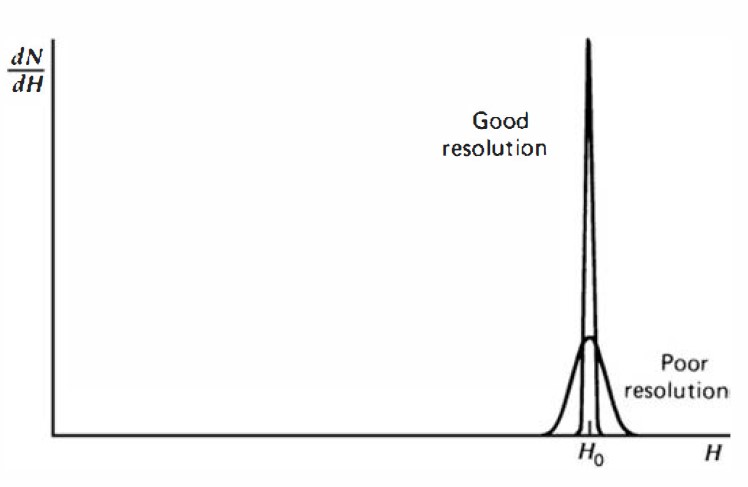
\includegraphics[width=0.7\textwidth]{Imagens/funcoesDeResposta.jpg}
			\caption{Funções de Resposta}
			\label{fig:funcoesDeResposta}
		\end{figure}

	Embora ambas as distribuições estejam centradas em torno do valor médio $H_0$, a largura da distribuição para a baixa resolução é muito maior. Esta largura reflete o fato de que foi registrada uma grande quantidade de flutuação de pulso a pulso embora a mesma energia tenha sido depositada para cada evento. Se a quantidade destas flutuações é for cada vez menor, a largura da distribuição será cada vez menor e a forma da curva se aproximará para uma função delta de dirac. 

	A definição para a resolução de energia de um detector pode ser observada na  \ref{fig:resolucaoDeEnergia}, onde a distribuição diferencial de amplitude de pulso é determinada para um detector submetido a um feixe monoenergético. 

			\begin{figure}[h]
				\centering
				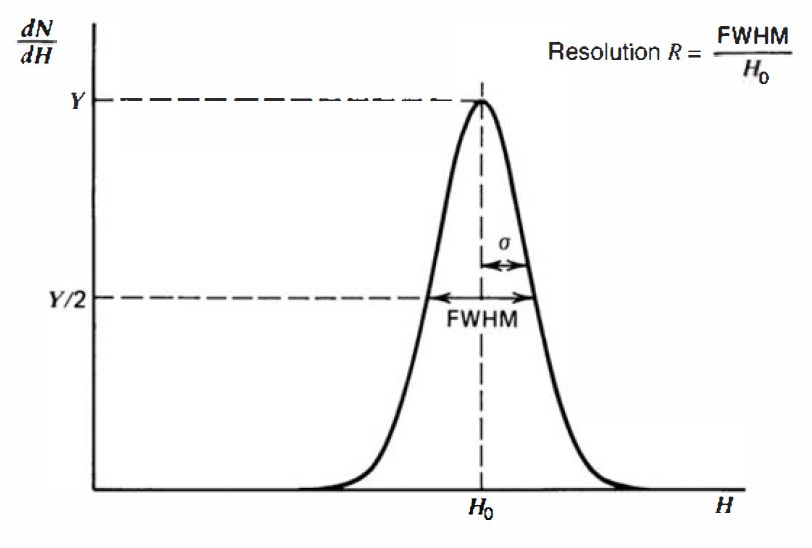
\includegraphics[width=0.7\textwidth]{Imagens/resolucaoDeEnergia.jpg}
				\caption{Resolução de Energia}
				\label{fig:resolucaoDeEnergia}
			\end{figure}


		A \textcolor{MediumOrchid}{\textit{\textbf{largura à meia altura}}} (FWHM,  do inglês \textit{Full Width at Half Maximum}) é definida como \textcolor{MediumOrchid}{\textit{\textbf{a largura da distribuição na metade da altura do pico relacionado a $H_0$}}}. Esta definição assume que \textcolor{MediumOrchid}{\textit{\textbf{qualquer sinal de fundo ou qualquer sinal contínuo que possa sobrepor o pico é negligenciável ou foi subtraído do sinal do pico}}}. A resolução R é uma grandeza adimensional, e  sua fração é convencionalmente expressa em percentual. Um diodo possui resolução energética de aproximadamente 1\% enquanto que detectores cintiladores possuem uma resolução energética variando entre ~3\% até $\sim$10\%.

		\textcolor{MediumOrchid}{\textit{\textbf{Quanto menor o valor para a resolução de energia, melhor será a habilidade do detector distinguir duas radiações cujas energias estão próximas uma da outra.}}} Uma regra prática é que o detector deve ser capaz de detectar duas energias separadas por mais de uma FWHW .

		Alguns fatores que causam flutuações na resposta de um detector são: desvios nas características de operação do detector durante a medição; fontes de ruídos aleatórias dentro do detector e do sistema de instrumentação e o ruído estatístico proveniente da natureza discreta do próprio sinal medido. 
		
		O \textcolor{MediumOrchid}{\textit{\textbf{ruído estatístico}}} representa a quantidade mínima de flutuação que não pode pode ser removida independente da qualidade do sistema de medição utilizado. O ruído estatístico surge devido ao fato de que \textcolor{MediumOrchid}{\textit{\textbf{a carga Q gerada dentro do detector devido a um quanta de radiação  não é uma variável contínua, mas sim um valor discreto do número de portadores de carga}}}. Pode ser feita uma estimativa da flutuação inerente da detecção assumindo que os portadores de carga criados se se aproximam de distribuição Gaussiana.

	\subsection*{Eficiência de Detecção}

		A \textcolor{MediumOrchid}{\textit{\textbf{eficiência de detecção}}} varia com o \textcolor{MediumOrchid}{\textit{\textbf{tipo de radiação}}} para o qual o detector será utilizado, sendo diferente para radiações diretamente ionizantes e indiretamente ionizantes.

		Quando uma radiação diretamente ionizante, como as partículas alfa e os elétrons, entra na cavidade do detector, causarão imediatamente ionizações e excitações no volume da cavidade, e após viajar uma pequena fração do seu alcance será liberado pares de íons suficientes que farão com que o pulso resultante seja grande o suficiente para ser registrado; Portanto, \textcolor{MediumOrchid}{\textit{\textbf{garantindo que o detector consiga detectar toda partícula carregada que entra em sua cavidade, pode-se dizer que o detector possuirá uma eficiência de contagem de 100\%}}}. 

		Enquanto que a radiação diretamente ionizante é imediatamente detectada entrar na cavidade do detector, para detectar uma radiação indiretamente ionizante, ela deve primeiramente sofrer uma interação significante no detector, para então ser possível detectá-la. Como estas radiações podem viajar largas distâncias entre as interações, alguns quantas dessa radiação não serão detectados e portanto \textcolor{MediumOrchid}{\textit{\textbf{a eficiência do detector será sempre menor que 100\%}}}.

		A eficiência na contagem é dividida entre:

			\begin{itemize}
				\item \textcolor{DarkTurquoise}{\textbf{Eficiência Absoluta ($\epsilon_{abs}$)}}, que é definida como a razão entre o número de pulsos registados \textcolor{MediumOrchid}{\textit{\textbf{$N_P$}}} e o número de partículas \textcolor{MediumOrchid}{\textit{\textbf{$N$}}} emitidas pela fonte, ou seja
				
					\begin{equation}
						\epsilon_{abs} = \frac{N_P}{N}
					\end{equation}
				
				A eficiência absoluta depende das \textcolor{MediumOrchid}{\textit{\textbf{propriedades do detector}}} e da \textcolor{MediumOrchid}{\textit{\textbf{geometria  utilizada na contagem}}}, sendo a principal componente a distância da fonte ao detector.
				
				\item \textcolor{DarkTurquoise}{\textbf{Eficiência Intrínseca ($\epsilon_{int}$)}}, que é definida como a razão entre o número de pulsos registrados \textcolor{MediumOrchid}{\textit{\textbf{$N_P$}}} e o Número de partículas \textcolor{MediumOrchid}{\textit{\textbf{$N_{in}$}}} que incidem no detector, ou seja:
				
					\begin{equation}
						\epsilon_{int} = \frac{N_P}{N_{in}}
					\end{equation}

				A eficiência intrínseca depende principalmente do \textcolor{MediumOrchid}{\textit{\textbf{material do detector, da energia da radiação, e da espessura de material do detector}}} na região de incidência do feixe. 
			\end{itemize}

		A relação entre as eficiências para uma fonte isotrópica é dada por:

			\begin{equation}
					\epsilon_{int} = \epsilon_{abs} \cdot \left(\frac{4 \pi}{\Omega}\right)
			\end{equation}

		\noindent onde $\Omega$ é o ângulo sólido do detector visto a partir da posição da fonte.

	\subsection*{Tempo Morto}

		Praticamente todos os detectores necessitam de uma quantidade de tempo mínima entre dois eventos para que ele possa registrar separadamente os dois pulsos, e essa limitação pode estar relacionada com a forma em si de realizar a detecção ou devido aos componentes eletrônicos do detector. Devido a natureza aleatória do decaimento radioativo, sempre existirá a possibilidade de um sinal verdadeiro não ser registrado por ocorrer muito próximo a outro evento. 

\section{Tipos de Detectores}

\subsection*{Detectores A Gás}

\subsubsection*{Câmaras de Ionização}



	Considere duas placas separadas por uma cavidade de ar com uma diferença de potencial entre elas (\ref{fig:camaraArLivre}); Caso um fóton atravesse entre as placas, esse fóton pode interagir com o nitrogênio presente no ar quebrando a molécula formando um par de elétron e ion de nitrogênio. O elétron irá se mover na direção da placa positiva enquanto que o íon de nitrogênio irá se mover na direção da placa negativa. Haverá então uma diferença de carga líquida que pode ser medida em um eletrômetro. Caso milhares de fótons atravessem o meio, a quantidade de fótons que atravessam esse meio pode ser medida através da diferença da carga dividida pela massa de ar dentro das placas. Algumas das ionizações que acontecem enviarão elétrons para fora das placas, mas algumas dessas ionizações acontecerão fora das placas e enviarão íons dentro da região das placas. A medida que a quantidade de íons que se move para fora da região é igual a quantidade de íons que entram dentro da região, ocorre o equilíbrio eletrônico. Quando a condição de equilíbrio eletrônico é alcançada estará medindo o kerma no ar, caso contrário não estará medindo o Kerma precisamente. 
	
	\begin{figure}[h]
		\centering
		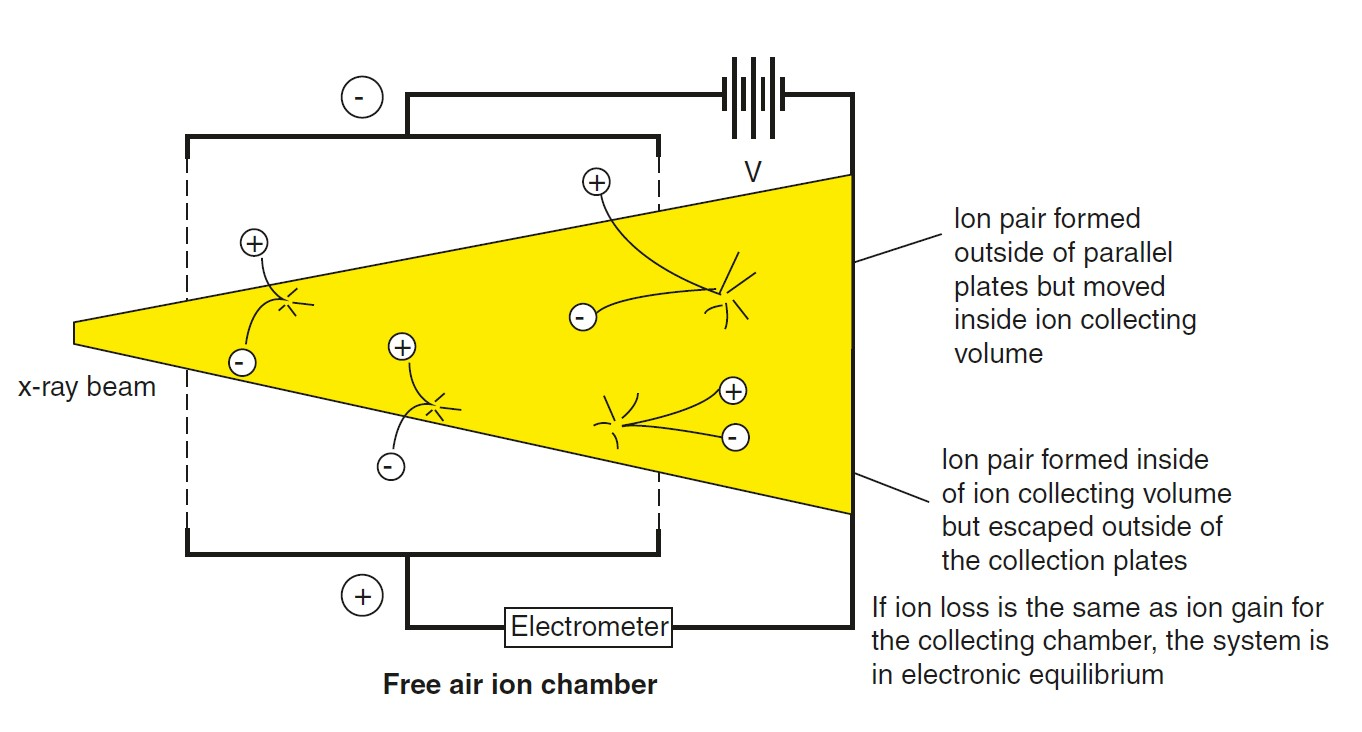
\includegraphics[width=0.8\textwidth]{Imagens/camaraArLivre.jpg}
		\caption{Câmara de Ar Livre}
		\label{fig:camaraArLivre}
	\end{figure}


	As câmaras de ionização estão disponíveis em várias formas e tamanhos, adaptadas a requisitos específicos, onde um esquema básico é apresentado na \ref{fig:}. Essas câmaras são dispositivos utilizados para medir a radiação ionizante, como raios-X ou feixes de partículas.

		\begin{figure}[h]
			\centering
			\fcolorbox{DarkTurquoise}{white}{%
				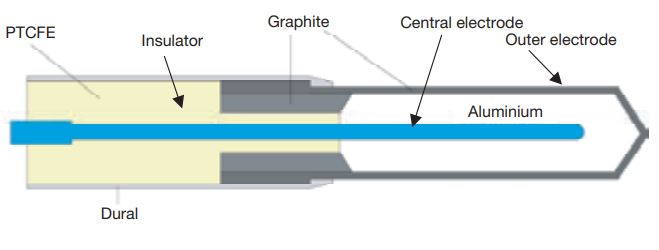
\includegraphics[width=0.5\textwidth]{Imagens/cameraFarmer.JPG}
			}%
			\caption{Projeto básico de uma câmara de ionização cilíndrica tipo Farmer.}
			\label{fig:}
		\end{figure}
		
	\begin{itemize}
		\item A estrutura básica de uma câmara de ionização consiste uma \textcolor{MediumOrchid}{\textit{\textbf{cavidade preenchida com gás, cercada por uma parede externa condutora}}}. No centro da câmara, encontra-se o \textcolor{MediumOrchid}{\textit{\textbf{eletrodo coletor}}}, que é responsável por coletar as cargas elétricas geradas pela radiação ionizante. A parede e o eletrodo coletor são separados por um \textcolor{MediumOrchid}{\textit{\textbf{isolante}}} de alta qualidade, projetado para minimizar a corrente de fuga quando uma voltagem de polarização é aplicada à câmara. Essa estrutura básica permite a detecção e quantificação da radiação ionizante.
		\item Um \textcolor{MediumOrchid}{\textit{\textbf{eletrodo de guarda}}} é tipicamente incluído na câmara de ionização. Esse eletrodo de guarda tem a função de \textcolor{MediumOrchid}{\textit{\textbf{minimizar ainda mais a corrente de fuga. Ele intercepta a corrente de fuga}}} e a redireciona para o terra, contornando o eletrodo coletor. Isso \textcolor{MediumOrchid}{\textit{\textbf{melhora a uniformidade do campo elétrico}}} dentro do volume ativo ou sensível da câmara, resultando em uma coleta de carga aprimorada. A presença do eletrodo de guarda é uma característica importante para garantir medições precisas e reduzir o impacto de correntes indesejadas durante o processo de medição.
		\item Ao utilizar \textcolor{MediumOrchid}{\textit{\textbf{câmaras de ionização não seladas}}}, é necessário aplicar correções de temperatura e pressão. Isso ocorre devido às variações na massa de ar dentro do volume da câmara, que são influenciadas por mudanças na temperatura ambiente e na pressão. Para garantir a precisão das medições, essas correções são aplicadas para considerar as alterações na densidade do ar, o que afeta a interação da radiação com o gás dentro da câmara.
	\end{itemize}

	Os \textcolor{MediumOrchid}{\textit{\textbf{eletrometros}}} são instrumentos projetados especificamente para medir correntes pequenas, geralmente da ordem de $10^{-9}$ $A$ ou inferiores. Quando usados em conjunto com uma câmara de ionização, os eletrometros funcionam como \textcolor{MediumOrchid}{\textit{\textbf{amplificadores}}} operacionais de realimentação negativa e de alto ganho. Isso significa que eles \textcolor{MediumOrchid}{\textit{\textbf{amplificam o sinal gerado pela câmara de ionização}}} para torná-lo mensurável e proporcionam \textcolor{MediumOrchid}{\textit{\textbf{um ganho de amplificação}}} preciso e estável. Os eletrometros também incorporam um resistor ou capacitor padrão no caminho da realimentação para medir a corrente da câmara ou a carga coletada ao longo de um intervalo de tempo fixo. Essa medição é fundamental para quantificar a radiação recebida e obter a dose absorvida.
	

\subsubsection*{Câmaras de Ar Livre}
		
	O padrão ouro para medida da radiação ionizante é a câmara de ionização de ar livre (\ref{fig:camaraArLivre}), porém sua construção requer tamanhos proporcionais ao alcance do elétron no ar, o que é muito grande para feixes de megavoltagem. Adicionalmente, uma vez que o meio é o ar livre sua construção é muito sensível à variações de temperatura, pressão, umidade e do campo elétrico. Por essas razões, as câmaras de ionização de ar livre só existem em laboratórios padrão. 

\subsubsection*{Câmaras do Tipo Dedal}

	Uma das câmaras de ionização cilíndricas mais amplamente utilizadas na dosimetria em radioterapia é a câmara de 0.6 cc originalmente projetada por Farmer e fabricada pela Baldwin, mas agora disponível em vários fornecedores. Essa câmara é frequentemente referida como tipo Farmer ou câmara tipo Thimble, devido à sua semelhança em forma a um dedal. Essa câmara foi projetada especificamente para \textcolor{MediumOrchid}{\textit{\textbf{aplicações em radioterapia}}} e se tornou um padrão na medição da dose absorvida em feixes radioterápicos.

	As câmaras cilíndricas estão disponíveis em vários tamanhos, com volumes ativos que variam de \textcolor{MediumOrchid}{\textit{\textbf{0.1 cc a 1 cc}}}. Essas câmaras são projetadas com um \textcolor{MediumOrchid}{\textit{\textbf{comprimento interno que não excede 25 mm}}} e um \textcolor{MediumOrchid}{\textit{\textbf{diâmetro interno não superior a 7 mm}}}. Essas dimensões são importantes para garantir uma \textcolor{MediumOrchid}{\textit{\textbf{resposta precisa e localizada}}} da câmara à radiação incidente. As paredes dessas câmaras são construídas com materiais de baixo número atômico (Z), o que garante a equivalência da interação da radiação com o ar. Além disso, uma capa de buildup de espessura aproximada de 0.5 \unit{g/cm^2} é incorporada ao projeto da câmara para calibração em condições de ar livre usando radiação de \ce{^{60}Co}.

	A construção da câmara busca manter características homogêneas e uniformes. No entanto, é comum que essas câmaras apresentem um eletrodo central de alumínio, com aproximadamente 1 mm de diâmetro. Esse eletrodo central tem a função de \textcolor{MediumOrchid}{\textit{\textbf{garantir uma resposta plana}}} e independente da energia, ou seja, uma \textcolor{MediumOrchid}{\textit{\textbf{resposta de dependência energética uniforme}}}.

	Para obter uma câmara de ionização mais compacta (comparado à câmara de ar livre), é necessário utilizar um \textcolor{MediumOrchid}{\textit{\textbf{eletrodo central e uma parede externa}}};  O número de elétrons entrando na cavidade deve ser o mesmo número de elétrons saindo da cavidade a fim de alcançar o equilíbrio eletrônico, e isto normalmente irá requerer uma cavidade de ar muito larga;	
	Porém, esta condição pode ser respeitada se as paredes que circundam a cavidade de ar forem feitas com um material muito mais denso mas ainda ter um número atômico semelhante ao número atômico das moléculas de ar; Com uma parede ``equivalente a ar denso'' em volta da cavidade de ar (para fornecer o buildup para o ar), a câmara pode ser feita pequena o suficiente para ser utilizada clinicamente.

	Caso a câmara seja pequena o suficiente de modo que ao ser inserida em um material a distribuição dos elétrons não seja alterada devido a presença da câmara, então a teoria cavitária de Braag-Gray pode ser utilizada para calcular a dose nessa região (Fig. \ref{fig:camaraDedal}.). 

		A Exposição para uma câmara dedal é calculada a partir da seguinte equação:
			\begin{equation}
				X = \frac{Q}{\rho \times \nu} \times \frac{1}{A}
			\end{equation}

		\begin{exemplo}[Onde]
			\begin{itemize}[label=\textcolor{CarnationPink}{$\star$}]
				\item \textcolor{DarkTurquoise}{$\mathbf{X}$} é a exposição;
				\item \textcolor{DarkTurquoise}{$\mathbf{Q}$} é a carga medida pelo eletrômetro;
				\item \textcolor{DarkTurquoise}{$\mathbf{\rho}$} é a densidade do ar;
				\item \textcolor{DarkTurquoise}{$\mathbf{\nu}$} é o volume de ar;
				\item \textcolor{DarkTurquoise}{$\mathbf{A}$} é o fator de correção para considerar a perturbação da câmara no meio (pouco menor que 1.00).
			\end{itemize}
		\end{exemplo}

		\begin{figure}[h]
			\centering
			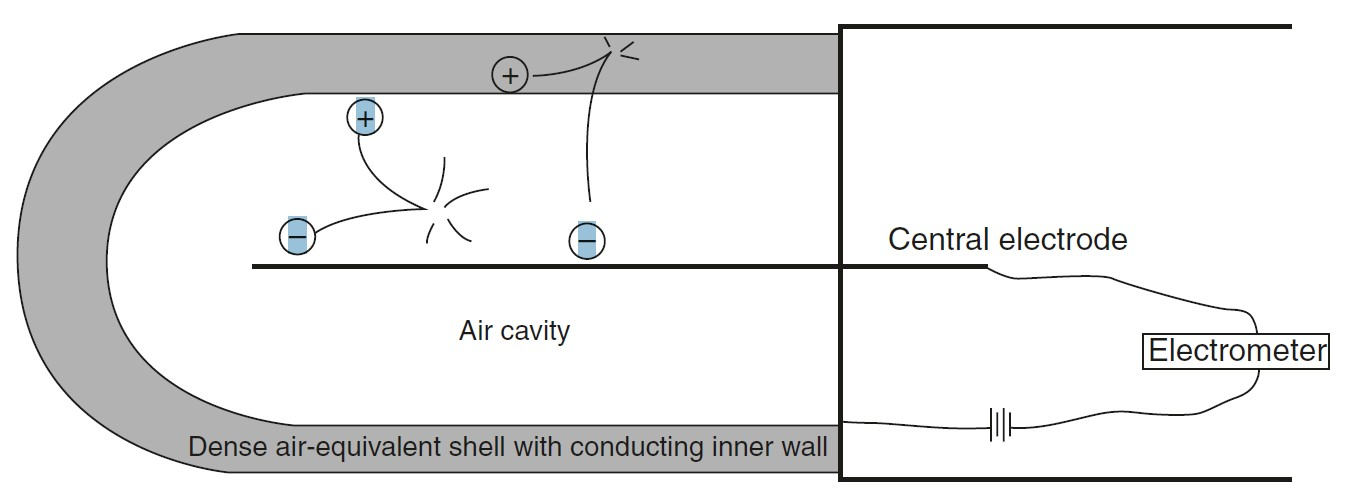
\includegraphics[width=0.5\textwidth]{Imagens/camaraDedal.jpg}
			\caption{Câmara dedal: constituída de um eletrodo central e uma parede condutora que pode ser utilizada para medir a carga. A parede feita de um material equivalente aos ar denso permite que a câmara tenha seu tamanho significativamente reduzido enquanto continua mantendo as condições de equilíbrio eletrônico e portanto medições precisas.}
			\label{fig:camaraDedal}
		\end{figure}

		Como a câmara do tipo dedal ainda continua sendo preenchida com ar, a densidade do ar dentro da cavidade ainda continuará sensível a variações de temperatura e pressão e portanto esses fatores devem ser considerados para a correção das leituras medidas.

\subsubsection*{Câmaras tipo Farmer}

	A câmara de ionização tipo Farmer tem algumas características que a distingue das demais câmaras de ionização cilíndricas:

	\begin{itemize}[label=\textcolor{CarnationPink}{$\blacktriangleright$}]
		\item Além dos eletrodos coletores de íons e elétrons, a câmara de ionização tipo Farmer possui um eletrodo de guarda. Esse eletrodo é geralmente um cilindro oco no centro da câmara, que ajuda a fornecer uma referência de potencial constante durante as medições.
		\item A geometria cilíndrica da câmara de ionização tipo Farmer é otimizada para garantir uma resposta de dose uniforme e uma boa representação da dose absorvida em tecidos. O tamanho da câmara também é projetado para ser adequado para uso em feixes de radiação.
	\end{itemize}

\subsubsection*{Câmaras de Placas Paralelas}


	Uma câmara de ionização de placas paralelas é composta por duas paredes planas, cada uma desempenhando uma função específica (apresentada esuematicamente na \ref{fig:camaraPp} onde estão destacados -- a: a altura (separação entre os eletrodos) da cavidade de ar. 1: o eletrodo polarizador. d: o diâmetro do eletrodo polarizador. 2: o eletrodo coletor. m: o diâmetro do eletrodo coletor. 3: o anel de guarda. g: a largura do anel de guarda.). Uma parede atua como a janela de entrada e o eletrodo polarizador, enquanto a outra funciona como a parede traseira e o eletrodo coletor. Essa configuração permite a interação da radiação com o gás contido entre as placas da câmara, gerando íons que são coletados pelo eletrodo coletor. Além disso, um sistema de anel de guarda é incluído para garantir uma geometria adequada e evitar influências indesejadas.

	\begin{wrapfigure}{r}{0.45\textwidth}
		\centering
		\fcolorbox{DarkTurquoise}{white}{%
			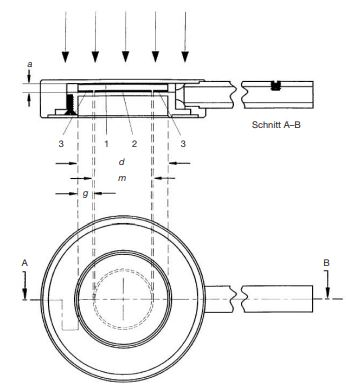
\includegraphics[width=0.37\textwidth]{Imagens/camaraPp.JPG}
		}%
		\caption{Câmara de ionização de placas paralelas.}
		\label{fig:camaraPp}
	\end{wrapfigure}
	
	A câmara de placas paralelas é especialmente adequada para \textcolor{MediumOrchid}{\textit{\textbf{aplicações de dosimetria envolvendo feixes de elétrons com energias abaixo de 10 MeV}}}. Isso ocorre porque esses feixes de elétrons têm uma taxa de deposição de energia alta o suficiente para gerar uma quantidade mensurável de carga coletada pela câmara. Além disso, essa configuração é utilizada para \textcolor{MediumOrchid}{\textit{\textbf{medir a dose superficial e a dose em profundidade na região de buildup de feixes de fótons de megavoltagem}}}. A câmara de placas paralelas é projetada para ser posicionada na pele do paciente ou em um fantoma de água, permitindo a medição da dose absorvida nessas regiões específicas.

	No entanto, é importante observar que certas câmaras de placas paralelas podem exigir \textcolor{MediumOrchid}{\textit{\textbf{correções significativas de perturbação de fluência}}}. Isso ocorre devido à \textcolor{MediumOrchid}{\textit{\textbf{largura inadequada do anel de guarda}}}, que pode influenciar a distribuição de radiação e a deposição de energia dentro da câmara. Para garantir medidas precisas, são necessárias correções adequadas para considerar essa perturbação da fluência e garantir a precisão das medições.

\subsubsection*{Câmaras de Ionização Tipo Poço}

	\begin{wrapfigure}{l}{0.48\textwidth}
		\centering
		\fcolorbox{DarkTurquoise}{white}{%
			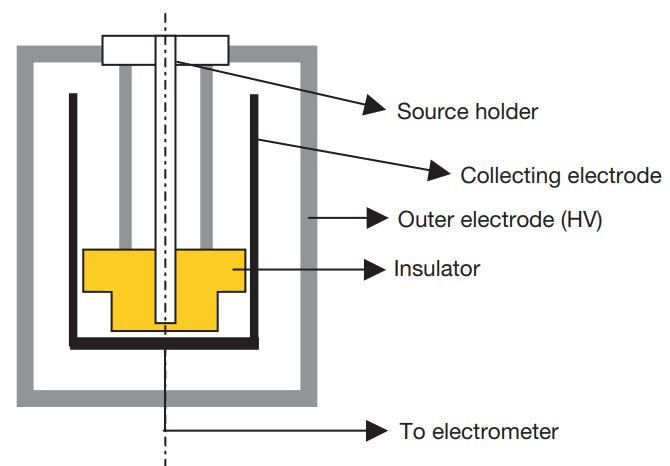
\includegraphics[width=0.43\textwidth]{Imagens/camaraPoco2.JPG}
		}%
		\caption{Projeto básico de uma câmara tipo poço utilizada em braquiterapia.}
		\label{fig:camaraPoco2}
	\end{wrapfigure}

	A braquiterapia envolve o uso de \textcolor{MediumOrchid}{\textit{\textbf{fontes de baixa taxa de kerma no ar}}}, o que requer câmaras com um volume adequado, geralmente em torno de \textcolor{MediumOrchid}{\textit{\textbf{250 cc}}} ou maior, para garantir uma sensibilidade adequada. Isso ocorre porque as fontes utilizadas na braquiterapia emitem radiação com taxas de dose relativamente baixas em comparação com as fontes utilizadas em teleterapia. Portanto, as câmaras utilizadas na dosimetria da braquiterapia precisam ser sensíveis o suficiente para detectar e quantificar a radiação emitida pelas fontes de braquiterapia. A \ref{fig:camaraPoco2} mostra o esquema de uma câmara de ionização do tipo poço.

	As câmaras do tipo poço ou câmaras reentrantes são \textcolor{MediumOrchid}{\textit{\textbf{adequadas para a calibração e padronização de fontes de braquiterapia}}}. Essas câmaras são projetadas com uma \textcolor{MediumOrchid}{\textit{\textbf{cavidade em forma de poço}}} que pode acomodar as fontes de tamanhos e formas típicas utilizadas na braquiterapia. Essas câmaras são \textcolor{MediumOrchid}{\textit{\textbf{calibradas em termos da taxa de kerma de ar de referência}}}, fornecendo medições precisas nas configurações de braquiterapia. A calibração é um processo importante para garantir que as medições realizadas com essas câmaras sejam confiáveis e consistentes.

\subsubsection*{Câmara de Extrapolação}

	As câmaras de extrapolação são um \textcolor{MediumOrchid}{\textit{\textbf{tipo de câmara de placas}}} paralelas que apresentam um volume sensível variável. Essas câmaras são comumente utilizadas na \textcolor{MediumOrchid}{\textit{\textbf{medição de doses superficiais em feixes de raios-X de ortovoltagem e megavoltagem}}}, bem como na \textcolor{MediumOrchid}{\textit{\textbf{dosimetria de raios $\beta$ e raios-X de baixa energia}}}. Isso significa que essas câmaras são adequadas para medir a dose absorvida na superfície do paciente em tratamentos com raios-X de diferentes energias. Além disso, elas também \textcolor{MediumOrchid}{\textit{\textbf{podem ser usadas para a dosimetria absoluta de radiação quando incorporadas diretamente em um fantoma tecido-equivalente}}}.

	Uma das vantagens das câmaras de extrapolação é sua \textcolor{MediumOrchid}{\textit{\textbf{capacidade de eliminar os efeitos de perturbação da cavidade causados por elétrons}}}. Nas medições realizadas com essas câmaras, são utilizadas \textcolor{MediumOrchid}{\textit{\textbf{várias espessuras de cavidade}}}, e os \textcolor{MediumOrchid}{\textit{\textbf{resultados são extrapolados para uma configuração de espessura zero}}}. Essa abordagem permite estimar a perturbação da cavidade associada a câmaras de placas paralelas de espessura finita. Isso é importante porque \textcolor{MediumOrchid}{\textit{\textbf{as câmaras de placas paralelas tradicionais podem apresentar perturbações nas medições devido à presença de elétrons que se acumulam nas proximidades da cavidade}}}. Com as câmaras de extrapolação, é possível corrigir esses efeitos indesejados e obter medições mais precisas e confiáveis da dose absorvida.


\subsubsection*{Câmaras Condensadoras}

	As câmaras condensadoras operam como capacitores e mede a queda na voltagem na presença da radiação com um fator de conversão conhecido para a queda de voltagem por roetgen de exposição. Esta câmara é sensível a fótons com energias até $\sim$ 2 MeV e são insensíveis a altas energias devido aos elétrons que saltam da haste de metal ou do material do isolante. Esses tipos de detectores não são mais utilizadas em radioterapia. 


\subsection*{Filmes Dosimétricos}

\subsubsection*{Filmes Radiográficos}

	O filme radiográfico de raios-X desempenha várias funções cruciais na radiologia diagnóstica, radioterapia e proteção radiológica. Ele atua como um \textcolor{MediumOrchid}{\textit{\textbf{detector de radiação, um dosímetro relativo e um dispositivo de visualização}}}. Isso significa que o filme radiográfico é uma ferramenta essencial em várias áreas da radiologia, sendo utilizado para capturar imagens de raios-X, medir a dose relativa de radiação, visualizar as estruturas anatômicas e armazenar registros de pacientes. O filme de raios-X não exposto consiste em uma base plástica fina revestida uniformemente em um ou ambos os lados com uma emulsão sensível à radiação, geralmente composta por grãos de brometo de prata (AgBr) suspensos em gelatina.

	\begin{exemplo}[Pontos importantes sobre o filme radiográfico:]
		\begin{itemize}
			\item A interação da radiação leva à \textcolor{DarkTurquoise}{\textit{\textbf{ionização dos grãos de \ce{AgBr}}}}, criando uma \textcolor{DarkTurquoise}{\textit{\textbf{imagem latente}}} no filme. Essa imagem se torna visível (escurecimento do filme) e permanente após o processamento.
			\item A quantidade de transmissão de luz através do filme é determinada pela sua opacidade e pode ser quantificada em termos de \textcolor{DarkTurquoise}{\textit{\textbf{densidade óptica}}} (OD) usando densitômetros.
			\item A OD é definida como \textcolor{DarkTurquoise}{\textit{\textbf{$OD = log10 (I_0/I)$}}}, onde $I_0$ é a intensidade inicial da luz e I é a intensidade transmitida através do filme. A OD está relacionada com a dose recebida.
			\item O filme radiográfico oferece excelente \textcolor{DarkTurquoise}{\textit{\textbf{resolução espacial bidimensional}}}, fornecendo informações sobre a distribuição espacial da radiação na área de interesse ou sobre a atenuação da radiação por objetos.
			\item A \textcolor{DarkTurquoise}{\textit{\textbf{faixa útil de dose}}} do filme é \textcolor{DarkTurquoise}{\textit{\textbf{limitada}}} e sua \textcolor{DarkTurquoise}{\textit{\textbf{dependência energética}}} é mais pronunciada para \textcolor{DarkTurquoise}{\textit{\textbf{fótons de energia mais baixa}}}. A resposta do filme depende de vários parâmetros, o que torna o processamento consistente um desafio.
			\item O filme é tipicamente usado para \textcolor{MediumOrchid}{\textit{\textbf{dosimetria qualitativa}}}, mas com \textcolor{DarkTurquoise}{\textit{\textbf{calibração adequada}}}, uso cuidadoso e análise, também pode ser utilizado para \textcolor{DarkTurquoise}{\textit{\textbf{avaliação de dose}}}.
			\item Vários tipos de filmes estão disponíveis para aplicações em radioterapia, incluindo filmes sem tela para verificação do tamanho do campo, filmes com tela de fósforo usados com simuladores e filmes com tela metálica usados em imagem portal.
			\item O filme não exposto exibe uma \textcolor{DarkTurquoise}{\textit{\textbf{OD de fundo}}} conhecida como \textcolor{DarkTurquoise}{\textit{\textbf{densidade de fundo (fog) (``fog density'') (OD\textsubscript{f})}}}, enquanto a densidade causada pela exposição à radiação é chamada de \textcolor{MediumOrchid}{\textit{\textbf{OD líquida}}}, obtida subtraindo-se a densidade de fundo (fog) da densidade medida.
			\item Leitores de OD incluem \textcolor{MediumOrchid}{\textit{\textbf{densitômetros de filme, densitômetros a laser e scanners automáticos de filmes}}}.
		\end{itemize}
	\end{exemplo}

	É importante que haja uma \textcolor{MediumOrchid}{\textit{\textbf{relação linear entre a dose de radiação recebida e a densidade óptica}}} registrada no filme radiográfico. No entanto, essa relação linear nem sempre é estritamente verdadeira. As emulsões presentes no filme radiográfico podem apresentar \textcolor{MediumOrchid}{\textit{\textbf{linearidade}}} em uma \textcolor{MediumOrchid}{\textit{\textbf{faixa limitada de doses}}} ou podem ser \textcolor{MediumOrchid}{\textit{\textbf{não lineares}}}. Para determinar como o filme responde à radiação, é necessário estabelecer uma \textcolor{MediumOrchid}{\textit{\textbf{curva sensitométrica}}}, também conhecida como curva característica ou curva H\&D (Hurter \& Driffield). Essa curva é uma \textcolor{MediumOrchid}{\textit{\textbf{representação gráfica da relação entre a dose de radiação e a densidade óptica registrada no filme}}}. Uma curva H\&D típica para um filme radiográfico é mostrada na \ref{fig:curvaHD}. Ela possui quatro regiões: (1) fundo (fog), em exposições baixas ou nulas; (2) início; (3) uma porção linear em exposições intermediárias; e (4) ombro e saturação em exposições altas.

	\begin{figure}[h]
		\centering
		\fcolorbox{DarkTurquoise}{white}{%
			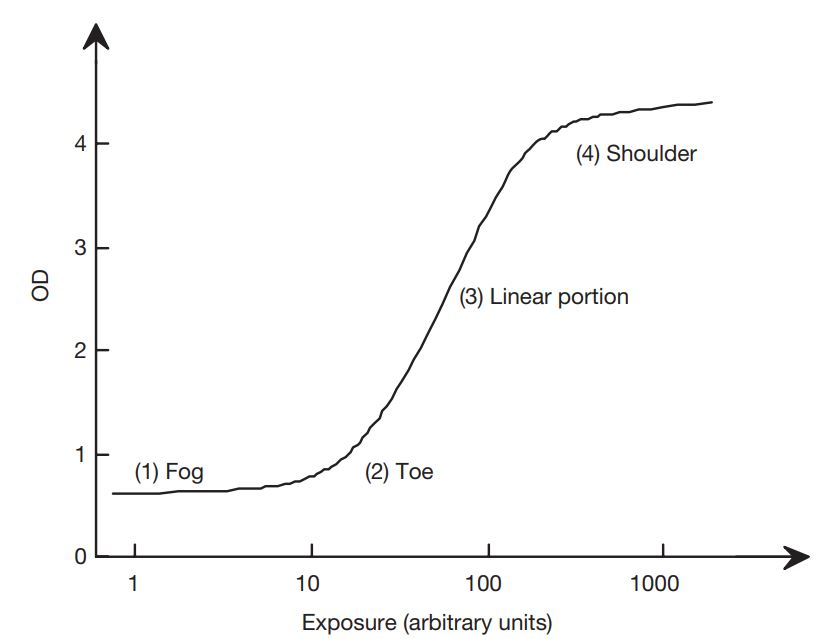
\includegraphics[width=0.5\textwidth]{Imagens/curvaHD.JPG}
		}%
		\caption{Curva H\&D.}
		\label{fig:curvaHD}
	\end{figure}

	Portanto, a curva sensitométrica do filme radiográfico é composta por quatro regiões distintas: fundo (fog), início, uma porção linear e ombro/saturação. A região da fundo (fog) é a região de baixas doses de radiação, onde a densidade óptica registrada no filme é principalmente devido a ruído de fundo e outras fontes de interferência, sendo referida como região de \textcolor{MediumOrchid}{\textit{\textbf{subexposição}}}. O início da curva representa o ponto em que a densidade óptica começa a aumentar linearmente com a dose de radiação. A \textcolor{MediumOrchid}{\textit{\textbf{porção linear}}} é referida como \textcolor{MediumOrchid}{\textit{\textbf{condições ótimas de medição}}}, onde se espera que haja uma relação linear entre a dose de radiação e a densidade óptica. Por fim, a região do ombro/saturação é onde a densidade óptica atinge um valor máximo e não aumenta significativamente mesmo com doses de radiação mais altas, sendo referida como região de \textcolor{MediumOrchid}{\textit{\textbf{superexposição}}}.

	\begin{exemplo}[Parâmetros importantes da resposta do filme radiográfico:]
		\begin{itemize}
			\item \textcolor{DarkTurquoise}{\textbf{Gamma:}} O gamma é um parâmetro que se refere à \textcolor{MediumOrchid}{\textit{\textbf{inclinação da porção linear da curva sensitométrica -- coeficiente angular}}} (curva H\&D). Ele indica o grau de linearidade entre a dose de radiação e a densidade óptica do filme. Quanto maior o valor de gamma, mais linear é a resposta do filme. Isso significa que uma pequena mudança na dose de radiação resultará em uma mudança proporcionalmente semelhante na densidade óptica registrada no filme.
			\item \textcolor{DarkTurquoise}{\textbf{Exposição:}}  A exposição do filme radiográfico deve ser selecionada de forma a garantir que \textcolor{MediumOrchid}{\textit{\textbf{todas as partes da radiografia estejam dentro da porção linear da curva sensitométrica}}}. Isso garante um contraste consistente para todas as densidades ópticas registradas no filme. Uma exposição inadequada pode resultar em regiões da imagem com baixo contraste ou superexpostas, dificultando a interpretação dos dados.
			\item \textcolor{DarkTurquoise}{\textbf{Latitude:}} A latitude do filme refere-se à \textcolor{MediumOrchid}{\textit{\textbf{faixa de exposições nas quais as densidades ópticas registradas no filme estarão dentro da região linear da curva sensitométrica}}}. Uma latitude ampla indica que o filme pode lidar com uma ampla gama de exposições, permitindo uma maior flexibilidade na configuração dos parâmetros de exposição durante a radioterapia.
			\item \textcolor{DarkTurquoise}{\textbf{Velocidade do filme:}} A velocidade do filme é determinada pela \textcolor{MediumOrchid}{\textit{\textbf{exposição necessária para produzir uma densidade óptica 1.0 vezes maior que a densidade de fundo (fog)}}}. Ela é um indicador da sensibilidade do filme à radiação. Um filme de alta velocidade requer menos exposição para atingir uma determinada densidade óptica em comparação com um filme de baixa velocidade. A escolha da velocidade do filme depende da aplicação específica e das necessidades clínicas.
		\end{itemize}
	\end{exemplo}

	% Em resumo, o filme radiográfico é amplamente utilizado na radioterapia com diversas aplicações. Ele é usado para medidas qualitativas e quantitativas, como avaliação visual de estruturas anatômicas e quantificação de densidades ópticas. Além disso, o filme é utilizado na dosimetria de feixes de elétrons, onde é importante garantir uma distribuição de dose adequada. O filme também desempenha um papel fundamental no controle de qualidade de máquinas de radioterapia, como verificar a congruência dos campos de luz e radiação, bem como determinar a posição do eixo do colimador usando o teste da estrela (star shot). Além disso, o filme é usado para verificar a técnica de tratamento em diversos phantomas, que são dispositivos projetados para simular tecidos ou órgãos do corpo humano. Por fim, o filme radiográfico é usado na técnica de imagem portal, que envolve a captura de imagens durante o tratamento de radioterapia para verificar a posição do paciente e a precisão do tratamento.
 
	Os filmes são constituídos e são utilizados na dosimetria das radiações da seguinte forma:

		\begin{itemize}
			\item \textcolor{DarkTurquoise}{\textbf{Estrutura do filme:}} Os filmes radiográficos são compostos por uma emulsão fotossensível, geralmente à base de prata, que é sensível à radiação ionizante. A emulsão contém grãos de brometo de prata halogenada dispersos em uma matriz gelatinosa.
			\item \textcolor{DarkTurquoise}{\textbf{Interação com a radiação:}} Quando a radiação ionizante, como raios-X ou raios gama, incide no filme, ocorre uma interação com os grãos de prata halogenada. Essa interação resulta na ionização e excitação dos átomos da prata presentes nos grãos.
			\item \textcolor{DarkTurquoise}{\textbf{Formação da Imagem Latente:}} A ionização e excitação dos átomos na emulsão fotossensível causam uma modificação estrutural nos grãos de prata halogenada (reação química), formando uma imagem latente. Essa imagem latente não é visível a olho nu.
			\item \textcolor{DarkTurquoise}{\textbf{Processamento do filme:}} O filme é submetido a um processo químico chamado de revelação, fixação e lavagem para revelar a imagem latente. A revelação envolve a redução dos grãos de prata ionizados a grãos metálicos de prata, enquanto a fixação remove os grãos não expostos e fixa os expostos. A lavagem final remove os resíduos químicos do processo.
			\item \textcolor{DarkTurquoise}{\textbf{Leitura da imagem:}} Após o processamento, a imagem resultante no filme radiográfico é visualizada. A densidade e a distribuição dos grãos de prata revelados refletem a quantidade de radiação absorvida pelo filme durante a exposição, onde a quantidade de radiação corresponde à quantidade de prata restante e, portanto, ao escurecimento.
		\end{itemize}

	\begin{tcolorbox}[width=\textwidth, colback={white}, colbacktitle={DarkTurquoise!50!white}, title={$\bigstar$ \LobsterTwo{Filme Radiográfico} $\bigstar$}, coltitle={CarnationPink}, colframe={DarkTurquoise}, fonttitle=\rmfamily\bfseries\Large, breakable]
		\textcolor{MediumOrchid}{\Large\LobsterTwo\textbf{Vantagens:}}

		\begin{itemize}[label=\textcolor{CarnationPink}{$\blacktriangleright$}]
			\item \textcolor{DarkTurquoise}{\textbf{Amplamente disponíveis:}} Os filmes radiográficos são amplamente utilizados na prática clínica e estão disponíveis em muitos centros de saúde e hospitais. Isso facilita o acesso a esses materiais para a dosimetria das radiações.
			\item \textcolor{DarkTurquoise}{\textbf{Baixo custo}}: Os filmes radiográficos são relativamente baratos em comparação com outros sistemas de dosimetria mais avançados. Isso os torna uma opção acessível, especialmente em conções com recursos limitados.
			\item \textcolor{DarkTurquoise}{\textbf{Registro permanente:}} Os filmes radiográficos fornecem um registro permanente da imagem e da distribuição de dose, permitindo uma documentação precisa dos resultados da dosimetria.
			\item \textcolor{DarkTurquoise}{\textbf{Alta resolução espacial:}} Os filmes radiográficos têm alta resolução espacial. A resolução espacial obtida por filmes radiográficos refere-se à capacidade do filme em capturar e reproduzir detalhes espaciais finos na imagem radiográfica. É uma medida da capacidade do filme em distinguir estruturas pequenas e próximas umas das outras; O que significa que eles podem fornecer detalhes precisos sobre a distribuição da dose em uma região específica. Ou seja, feixes de elétrons e feixes de fótons de megavoltagem podem ter suas isodoses medidas com relativa precisão e principalmente a forma de um feixe pode ser determinada.
			\item \textcolor{DarkTurquoise}{\textbf{Sensibilidade à radiação:}} Os filmes radiográficos têm uma resposta sensível à radiação ionizante, o que os torna úteis para medir uma ampla faixa de radiação.
		\end{itemize}

		\textcolor{MediumOrchid}{\Large\LobsterTwo\textbf{Desvantagens:}}

		\begin{itemize}[label=\textcolor{CarnationPink}{$\blacktriangleright$}]
			\item \textcolor{DarkTurquoise}{\textbf{Processamento químico}}: Os filmes radiográficos requerem processamento químico para revelar a imagem latente, o que pode ser demorado e exigir instalações específicas.
			\item \textcolor{DarkTurquoise}{\textbf{Resposta não linear:}} Os filmes radiográficos têm uma resposta não linear à radiação, o que significa que a densidade óptica dos grãos revelados pode não ser diretamente proporcional à dose absorvida. Isso requer uma calibração cuidadosa para obter resultados precisos.
			\item \textcolor{DarkTurquoise}{\textbf{Efeito de sobreposição:}} Quando múltiplos filmes são utilizados em conjunto para medir distribuições de dose complexas, pode haver sobreposição entre as imagens, dificultando a interpretação precisa dos resultados.
			\item \textcolor{DarkTurquoise}{\textbf{Limitações de tempo e temperatura:}} Os filmes radiográficos podem ser sensíveis ao tempo e à temperatura, o que pode afetar a estabilidade e a precisão das medições. O armazenamento e a manipulação adequadas são essenciais para garantir resultados confiáveis, além disso os filmes são sensíveis à luz visível, podendo ser contaminados.
			\item \textcolor{DarkTurquoise}{\textbf{Dificuldade na automação e análise:}} A análise dos filmes radiográficos geralmente requer um processo manual, o que pode ser demorado e sujeito a erros. Além disso, a automação e a análise objetiva podem ser desafiadoras devido à natureza analógica dos filmes.
		\end{itemize}

	\end{tcolorbox}

\subsubsection*{Filmes Radiocrômicos}

	O filme radiocrômico é um tipo de filme utilizado na dosimetria em radioterapia. O filme GafChromic é um exemplo comumente utilizado nesse contexto. Ao contrário do filme radiográfico tradicional, o filme radiocrômico não possui cor inicialmente, e \textcolor{MediumOrchid}{\textit{\textbf{apresenta uma composição que se assemelha ao tecido humano}}}. Essa composição inclui aproximadamente \textcolor{MediumOrchid}{\textit{\textbf{9.0\% de hidrogênio, 60.6\% de carbono, 11.2\% de nitrogênio e 19.2\% de oxigênio}}}. O filme radiocrômico serve como um \textcolor{MediumOrchid}{\textit{\textbf{dosímetro relativo}}}. Com uma calibração cuidadosa e consideração das condições ambientais, é possível alcançar uma precisão melhor que 3\%.

	Quando o filme radiocrômico é exposto à radiação, ocorre um \textcolor{MediumOrchid}{\textit{\textbf{processo de polimerização}}} de um corante especial presente nele. Esse processo resulta na absorção de luz, e a transmissão de luz através do filme pode ser medida utilizando um densitômetro apropriado. A principal característica visual resultante desse processo de polimerização é a \textcolor{MediumOrchid}{\textit{\textbf{cor azul}}} que surge no filme após a exposição à radiação.

	Uma das vantagens notáveis do uso do filme radiocrômico é que ele \textcolor{MediumOrchid}{\textit{\textbf{se desenvolve automaticamente, não necessitando de revelador ou fixador}}}. Isso simplifica o processo de uso em comparação com filmes radiográficos tradicionais, que exigem etapas de processamento adicionais. Além disso, o filme radiocrômico oferece \textcolor{MediumOrchid}{\textit{\textbf{alta resolução espacial}}} devido à sua natureza sem grão, o que o torna adequado para medições em regiões com gradientes de dose elevados, como campos estereotáticos e próximos a fontes de braquiterapia.

	Outras vantagens do filme radiocrômico em relação aos filmes radiográficos tradicionais incluem \textcolor{MediumOrchid}{\textit{\textbf{facilidade de uso, eliminação da necessidade de instalações de câmara escura, cassetes de filme e processamento de filme}}}. Ele também é \textcolor{MediumOrchid}{\textit{\textbf{independente da taxa de dose}}}, o que significa que sua resposta não é afetada pela variação da taxa de entrega da radiação. Além disso, o filme radiocrômico possui melhores características de energia em comparação com os filmes radiográficos, exceto para raios-X de baixa energia abaixo de 25 kV.

	Em relação à estabilidade, os filmes radiocrômico são \textcolor{MediumOrchid}{\textit{\textbf{relativamente insensíveis às condições ambientais}}}, embora seja importante evitar a exposição excessiva à umidade. É importante ressaltar que esses filmes são geralmente \textcolor{MediumOrchid}{\textit{\textbf{menos sensíveis do que os filmes radiográficos}}}, tornando-os mais adequados para faixas de dose mais altas. No entanto, em doses mais altas, pode ocorrer uma \textcolor{MediumOrchid}{\textit{\textbf{não-linearidade na resposta à dose}}}, e essa não-linearidade precisa ser corrigida para garantir uma medição precisa e confiável.

	% O filme radiocrômico é um tipo especial de filme que muda de cor quando exposto à radiação ionizante. Diferente dos filmes radiográficos convencionais, que são sensíveis à luz, os filmes radiocrômicos não são sensíveis à luz visível (embora ainda seja sensível à luz UV).

	% A composição dos filmes radiocrômicos pode variar dependendo do fabricante, mas geralmente eles são compostos por uma matriz polimérica contendo um material sensibilizador. O material sensibilizador é responsável por reagir com a radiação ionizante e causar uma mudança na cor do filme. Quando o filme radiocrômico é exposto à radiação ionizante, ocorrem interações entre os raios X, raios gama ou outras partículas da radiação e o material sensibilizador. Essas interações podem resultar em danos na estrutura molecular do material sensibilizador, que por sua vez causam mudanças na absorção ou reflexão da luz pelo filme. A mudança na absorção ou reflexão da luz afeta a cor percebida do filme. A quantidade de radiação absorvida determinará a magnitude da mudança de cor. Através da análise dessa mudança de cor, é possível determinar a dose de radiação absorvida pelo filme.

	Portanto, o processo de dosimetria utilizando filmes radiocrômicos ocorre da seguinte maneira:
		\begin{enumerate}
			\item \textcolor{DarkTurquoise}{\textbf{Exposição à radiação:}} O filme radiocrômico é colocado em uma região onde a radiação ionizante será medida. A radiação interage com o material sensibilizador no filme, causando danos ou modificando a estrutura molecular do material.
			\item \textcolor{DarkTurquoise}{\textbf{Mudança de cor:}} A interação da radiação provoca uma mudança na cor do filme. A magnitude da mudança de cor está relacionada à quantidade de radiação absorvida pelo filme.
			\item \textcolor{DarkTurquoise}{\textbf{Análise da mudança de cor:}} Após a exposição, o filme radiocrômico é analisado para determinar a mudança de cor. Isso pode ser feito visualmente, comparando a cor do filme antes e depois da exposição, ou por meio de equipamentos específicos que medem a absorção de luz em diferentes comprimentos de onda.
			\item \textcolor{DarkTurquoise}{\textbf{Calibração:}} Antes do uso do filme radiocrômico como dosímetro, é necessário realizar uma calibração. Isso envolve a exposição do filme a uma série conhecida de doses de radiação e a correlação entre a mudança de cor e a dose absorvida é estabelecida.
			\item \textcolor{DarkTurquoise}{\textbf{Interpretação da dose:}} Com base na mudança de cor medida no filme radiocrômico, é possível determinar a dose de radiação absorvida pelo filme. A relação entre a mudança de cor e a dose é utilizada para fazer essa determinação.
		\end{enumerate}

	\begin{tcolorbox}[width=\textwidth, colback={white}, colbacktitle={DarkTurquoise!50!white}, title={$\bigstar$ \LobsterTwo{Filme Radiocrômico} $\bigstar$}, coltitle={CarnationPink}, colframe={DarkTurquoise}, fonttitle=\rmfamily\bfseries\Large, breakable]

		\textcolor{MediumOrchid}{\Large\LobsterTwo\textbf{Vantagens:}}
		\begin{itemize}[label=\textcolor{CarnationPink}{$\blacktriangleright$}]
			\item \textcolor{DarkTurquoise}{\textbf{Alta resolução espacial:}} Os filmes radiocrômicos possuem alta resolução espacial, o que significa que eles podem fornecer informações detalhadas sobre a distribuição espacial da dose de radiação. Isso é especialmente útil em aplicações onde é necessário mapear a distribuição precisa da dose em uma área específica.
			\item \textcolor{DarkTurquoise}{\textbf{Sensibilidade a diferentes tipos de radiação:}} Os filmes radiocrômicos podem ser sensíveis a uma ampla gama de radiações ionizantes, incluindo raios X, raios gama, partículas alfa, partículas beta, entre outras. Isso os torna versáteis em termos de aplicação, permitindo a dosimetria de diferentes tipos de radiação.
			\end{itemize}
		\textcolor{MediumOrchid}{\Large\LobsterTwo\textbf{Desvantagens:}}

		\begin{itemize}[label=\textcolor{CarnationPink}{$\blacktriangleright$}]
			\item \textcolor{DarkTurquoise}{\textbf{Calibração e interpretação complexas:}} A calibração dos filmes radiocrômicos requer procedimentos cuidadosos para correlacionar a mudança de cor com a dose de radiação absorvida. Além disso, a interpretação dos resultados também pode ser complexa, exigindo equipamentos específicos e experiência adequada.
			\item \textcolor{DarkTurquoise}{\textbf{Limitações de faixa de dose:}} Os filmes radiocrômicos podem ter limitações em termos de faixa de dose que podem ser medidos com precisão. Cada tipo de filme radiocrômico tem sua própria faixa de dose linear e acima ou abaixo dessa faixa, a resposta pode não ser linear ou pode ocorrer saturação.
			\item \textcolor{DarkTurquoise}{\textbf{Limitação de tempo de resposta:}} Os filmes radiocrômicos podem ter um tempo de resposta relativamente lento para desenvolver completamente a mudança de cor após a exposição à radiação. Dependendo do tipo de filme e das condições de processamento, pode levar horas, para que a mudança de cor se estabilize completamente. Essa limitação de tempo de resposta pode ser inconveniente em situações onde a resposta imediata é necessária, especialmente em ambientes de monitoramento em tempo real ou em casos de acidentes radiológicos.
		\end{itemize}
	\end{tcolorbox}


\subsection*{Dosímetros Luminescentes}

	A luminescência é um fenômeno exibido por certos materiais quando absorvem radiação, no qual uma parte da \textcolor{MediumOrchid}{\textit{\textbf{energia absorvida é armazenada em estados metaestáveis}}}. Essa energia é posteriormente liberada na forma de luz ultravioleta, visível ou infravermelha. Existem dois tipos principais de luminescência: \textcolor{MediumOrchid}{\textit{\textbf{fluorescência}}} e \textcolor{MediumOrchid}{\textit{\textbf{fosforescência}}}, e a diferença entre eles reside no tempo de atraso entre a estimulação e a emissão de luz. A fluorescência ocorre com um atraso de tempo de $10^{-10}$ a $10^{-8}$ segundos, enquanto a fosforescência tem um atraso de tempo superior a $10^{-8}$ segundos. A fosforescência pode ser acelerada através de estimulação adequada, como calor ou luz.

	Quando o \textcolor{MediumOrchid}{\textit{\textbf{calor}}} é o agente estimulante, o fenômeno é chamado de \textcolor{MediumOrchid}{\textit{\textbf{termoluminescência (TL)}}}, e o material utilizado para fins de dosimetria é denominado material termoluminescente ou \textcolor{MediumOrchid}{\textit{\textbf{TLD}}} (dosímetro termoluminescente). Por outro lado, quando a luz é o agente estimulante, o fenômeno é conhecido como \textcolor{MediumOrchid}{\textit{\textbf{luminescência estimulada opticamente (OSL, do inglês \textit{Optically Stimulated Luminescence})}}}.

	Durante a interação dos fótons com a matéria, partículas carregadas secundárias altamente energéticas, principalmente elétrons, são responsáveis pela deposição de energia do fóton. Em materiais sólidos cristalinos, essas partículas carregadas secundárias liberam uma grande quantidade de elétrons livres de baixa energia e lacunas por meio da ionização de átomos e íons. Esses elétrons livres e lacunas podem recombinar-se entre si ou ficar \textcolor{MediumOrchid}{\textit{\textbf{aprisionados em armadilhas de elétrons ou lacunas}}} presentes na rede cristalina. Essas armadilhas podem ser \textcolor{MediumOrchid}{\textit{\textbf{intrínsecas}}} ao material ou \textcolor{MediumOrchid}{\textit{\textbf{introduzidas como imperfeições de rede, como lacunas ou impurezas}}}. Existem dois tipos gerais de armadilhas: \textcolor{MediumOrchid}{\textit{\textbf{armadilhas de armazenamento}}} e \textcolor{MediumOrchid}{\textit{\textbf{centros de recombinação}}}.

	Uma armadilha de armazenamento \textcolor{MediumOrchid}{\textit{\textbf{captura portadores de carga livres}}} e, posteriormente, os \textcolor{MediumOrchid}{\textit{\textbf{libera}}} durante dois processos diferentes: \textcolor{MediumOrchid}{$\mathbf{(i)}$} aquecimento, resultando no fenômeno de termoluminescência, ou \textcolor{MediumOrchid}{$\mathbf{(ii)}$} irradiação com luz, resultando no processo de OSL.

	Quando um portador de carga é liberado de uma \textcolor{MediumOrchid}{\textit{\textbf{armadilha de armazenamento}}}, ele pode recombinar-se com um portador de carga aprisionado de polaridade oposta em um centro de recombinação, também conhecido como \textcolor{MediumOrchid}{\textit{\textbf{centro de luminescência}}}. A energia resultante da recombinação é parcialmente emitida como \textcolor{MediumOrchid}{\textit{\textbf{luz ultravioleta, visível ou infravermelha}}}, e essa luz pode ser medida usando \textcolor{MediumOrchid}{\textit{\textbf{fotodiodos}}} ou \textcolor{MediumOrchid}{\textit{\textbf{tubos fotomultiplicadores (PMTs)}}}. Esses dispositivos detectam a luz emitida pelos centros de luminescência, permitindo assim a quantificação da quantidade de radiação absorvida pelo material luminescente, o que é fundamental para a dosimetria em radioterapia.

\subsubsection*{Dosímetros Termoluminescentes (TLD)}

	A termoluminescência é um fenômeno de \textcolor{MediumOrchid}{\textit{\textbf{fosforescência}}} que é ativado \textcolor{MediumOrchid}{\textit{\textbf{termicamente}}}, ou seja, é estimulado pelo aquecimento do material. A termoluminescência possui diversas aplicações práticas, desde a datação de cerâmicas arqueológicas até a dosimetria da radiação, o que a torna uma área de grande importância na física médica.

	Um modelo fenomenológico útil para entender o mecanismo da termoluminescência é a \textcolor{MediumOrchid}{\textit{\textbf{teoria de bandas para sólidos}}} (\ref{fig:tldOsld}). Nesse modelo, as armadilhas de armazenamento e os centros de recombinação são os pontos chaves. Cada tipo de armadilha é caracterizado por uma \textcolor{MediumOrchid}{\textit{\textbf{energia de ativação}}}, que é a profundidade da armadilha e depende das propriedades do sólido cristalino e da natureza da armadilha. Essas armadilhas estão localizadas na faixa de energia entre a banda de valência e a banda de condução do material.As \textcolor{MediumOrchid}{\textit{\textbf{armadilhas de elétrons}}} são estados localizados logo \textcolor{MediumOrchid}{\textit{\textbf{abaixo da banda de condução}}}, enquanto as \textcolor{MediumOrchid}{\textit{\textbf{armadilhas de lacunas}}} são estados localizados logo \textcolor{MediumOrchid}{\textit{\textbf{acima da banda de valência}}}. Antes da irradiação, essas armadilhas estão vazias, o que significa que as armadilhas de lacunas contêm elétrons, e as armadilhas de elétrons estão desocupadas.

	Durante a irradiação com radiação ionizante, as \textcolor{MediumOrchid}{\textit{\textbf{partículas carregadas secundárias}}} do processo de interação entre a radiação e o material elevam \textcolor{MediumOrchid}{\textit{\textbf{elétrons}}} da \textcolor{MediumOrchid}{\textit{\textbf{banda de valência}}} para a \textcolor{MediumOrchid}{\textit{\textbf{banda de condução}}}, deixando uma lacuna livre na banda de valência. Essas partículas carregadas também podem preencher uma armadilha de lacuna vazia, ocupando a armadilha de lacuna. Esse processo de \textcolor{MediumOrchid}{\textit{\textbf{transferência de elétrons e lacunas}}} é responsável pela \textcolor{MediumOrchid}{\textit{\textbf{absorção de energia}}} da radiação no material.

	Após a irradiação, os \textcolor{MediumOrchid}{\textit{\textbf{elétrons}}} e as \textcolor{MediumOrchid}{\textit{\textbf{lacunas}}} ficam presos nas armadilhas, onde permanecem em um \textcolor{MediumOrchid}{\textit{\textbf{estado metaestável}}}. Quando o material é aquecido, a \textcolor{MediumOrchid}{\textit{\textbf{energia térmica}}} fornecida é suficiente para que os elétrons e as lacunas aprisionados nas armadilhas escapem delas e \textcolor{MediumOrchid}{\textit{\textbf{retornem às bandas de valência e condução}}}, respectivamente. Durante esse processo de escape, a energia armazenada é liberada na forma de luz visível ou ultravioleta, que pode ser medida e quantificada usando \textcolor{MediumOrchid}{\textit{\textbf{fotodiodos}}} ou \textcolor{MediumOrchid}{\textit{\textbf{tubos fotomultiplicadores (PMTs)}}}. Essa emissão de luz é o fenômeno da termoluminescência.

	Após a absorção da radiação e a formação de elétrons e lacunas, o sistema pode atingir o \textcolor{MediumOrchid}{\textit{\textbf{equilíbrio térmico}}} por meio de diferentes mecanismos:

	\begin{itemize}
		\item \textcolor{DarkTurquoise}{\textbf{Recombinação dos portadores de carga:}} Os elétrons e lacunas podem recombinar-se, resultando na liberação da energia de recombinação na forma de calor. Esse processo ocorre quando um \textcolor{MediumOrchid}{\textit{\textbf{elétron livre}}} e uma \textcolor{MediumOrchid}{\textit{\textbf{lacuna}}} se \textcolor{MediumOrchid}{\textit{\textbf{combinam}}}, aniquilando um ao outro. A \textcolor{MediumOrchid}{\textit{\textbf{energia}}} que estava associada aos portadores de carga é convertida em \textcolor{MediumOrchid}{\textit{\textbf{energia térmica}}}, elevando a temperatura do material.

		\item \textcolor{DarkTurquoise}{\textbf{Recombinação com emissão de fluorescência óptica:}} Um elétron livre pode \textcolor{MediumOrchid}{\textit{\textbf{recombinar-se}}} com um portador de carga aprisionado de sinal oposto em um \textcolor{MediumOrchid}{\textit{\textbf{centro de luminescência}}}, também conhecido como centro de recombinação. Essa recombinação resulta na emissão de \textcolor{MediumOrchid}{\textit{\textbf{luz visível}}}, conhecida como \textcolor{MediumOrchid}{\textit{\textbf{fluorescência óptica}}}. Nesse caso, parte da energia de recombinação é convertida em luz, e o sistema atinge o equilíbrio térmico por meio dessa emissão.

		\item \textcolor{DarkTurquoise}{\textbf{Armazenamento em armadilhas:}} Os elétrons livres podem ficar aprisionados em \textcolor{MediumOrchid}{\textit{\textbf{armadilhas de armazenamento}}}, que são locais na estrutura do material onde os elétrons podem ser capturados e armazenados. Essas armadilhas podem ser intrínsecas ao material ou introduzidas como imperfeições da rede cristalina. O aprisionamento dos elétrons nas armadilhas ocorre devido à interação com defeitos ou impurezas no material.
	\end{itemize}

	\noindent \textcolor{MediumOrchid}{\Large\LobsterTwo\textbf{Sistemas de Dosimetria Termoluminescente}}

	\

	Os sistemas de dosimetria termoluminescente (TLD) são amplamente utilizados em diversas aplicações médicas devido à sua capacidade de medir doses de radiação com precisão. Existem diferentes tipos de materiais TLD empregados em dosimetria médica, sendo os mais comuns \textcolor{MediumOrchid}{\textit{\textbf{\ce{LiF}:\ce{Mg},ce{Ti}, \ce{LiF}:\ce{Mg},\ce{Cu},\ce{P} e \ce{Li2B4O7}:\ce{Mn}}}}, devido à sua equivalência com tecido humano. Além disso, materiais como \textcolor{MediumOrchid}{\textit{\textbf{\ce{CaSO4}:\ce{Dy}, \ce{Al2O3}:\ce{C} e \ce{CaF2}:\ce{Mn}}}} são utilizados por sua alta sensibilidade.

	Os materiais TLD podem ser encontrados em diferentes formas, como pó, chips, hastes e fitas. Antes de serem utilizados para a medição de doses, os TLDs passam por um processo de \textcolor{MediumOrchid}{\textit{\textbf{recozimento}}}, no qual são \textcolor{MediumOrchid}{\textit{\textbf{aquecidos}}} para apagar qualquer \textcolor{MediumOrchid}{\textit{\textbf{sinal residual}}} que possa estar presente. É fundamental seguir ciclos de recozimento bem estabelecidos e reproduzíveis, que envolvem taxas específicas de aquecimento e resfriamento, a fim de garantir a eficiência e a precisão dos resultados de dosimetria.

	Um sistema básico de leitura de TLD consiste em um \textcolor{MediumOrchid}{\textit{\textbf{suporte}}} no qual o \textcolor{MediumOrchid}{\textit{\textbf{TLD é colocado e aquecido}}}. A luz termoluminescente emitida pelo TLD, quando aquecido, é detectada por um \textcolor{MediumOrchid}{\textit{\textbf{tubo fotomultiplicador (PMT)}}}, que converte essa luz em um \textcolor{MediumOrchid}{\textit{\textbf{sinal elétrico proporcional}}} à intensidade da luz emitida. O sinal elétrico do PMT é linearmente proporcional à fluência de fótons detectada pelo TLD. Um eletrometro é utilizado para registrar o sinal do PMT como uma carga ou corrente, fornecendo uma medida da dose de radiação absorvida pelo TLD. Um diagrama esquemático básico de um leitor TLD é mostrado na \ref{fig:leitorTld}.

	\begin{figure}[h]
		\centering
		\fcolorbox{DarkTurquoise}{white}{%
			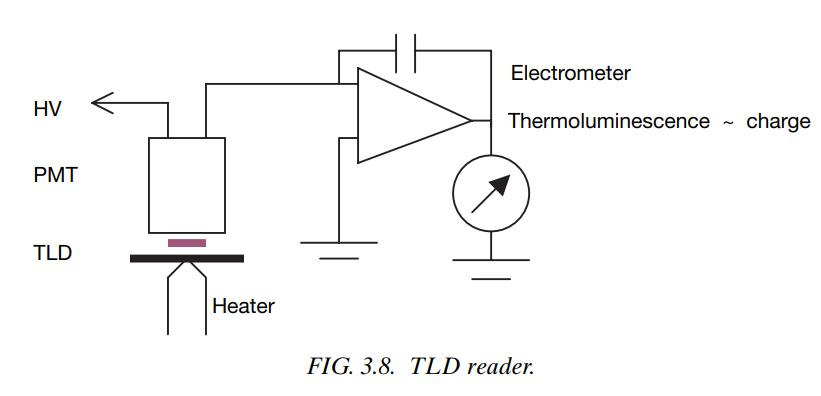
\includegraphics[width=0.5\textwidth]{Imagens/leitorTld.JPG}
		}%
		\caption{Leitora de TLD.}
		\label{fig:leitorTld}
	\end{figure}

	\begin{exemplo}[Pontos sobre a leitura do TLD:]
		\begin{itemize}
			\item \textcolor{DarkTurquoise}{\textit{\textbf{A intensidade da emissão de termoluminescência de um dosímetro TLD depende da temperatura $T$}}}. Mantendo uma taxa de aquecimento constante, a temperatura $T$ pode ser proporcional ao tempo $t$. Quando temos acesso a um registro de saída do sistema de medição do TLD, podemos plotar a intensidade da termoluminescência em função do tempo, resultando em uma curva chamada curva de brilho do TLD. Alternativamente, podemos plotar a luz emitida em função da temperatura do cristal, obtendo um termograma de termoluminescência. Essas curvas fornecem informações sobre as propriedades do TLD e permitem a extração de dados relevantes (\ref{fig:curvLiF}).
		  
			\item \textcolor{DarkTurquoise}{\textit{\textbf{Os picos observados na curva de brilho estão relacionados às profundidades das armadilhas que são responsáveis pela emissão da termoluminescência}}}. Cada pico corresponde a uma armadilha específica no material TLD. Ao analisar as posições e as características desses picos, é possível identificar as propriedades das armadilhas, o que contribui para uma melhor compreensão do comportamento do TLD.
		  
			\item \textcolor{DarkTurquoise}{\textit{\textbf{No caso específico dos TLDs de \ce{LiF}:\ce{Mg},\ce{Ti}, o principal pico dosimétrico na curva de brilho ocorre geralmente entre \SI{180}{\celsius} e \SI{260}{\celsius}}}}, e é nessa faixa que é realizada a dosimetria. A escolha da temperatura do pico dosimétrico leva em consideração a necessidade de evitar interferência da temperatura ambiente e da emissão de corpo negro do suporte de aquecimento.
		  
			\item \textcolor{DarkTurquoise}{\textit{\textbf{O sinal total de termoluminescência emitido, representado pela área sob a parte apropriada da curva de brilho, pode ser correlacionado com a dose absorvida por meio de uma calibração adequada}}}. Para isso, é necessário realizar experimentos de calibração utilizando diferentes doses conhecidas de radiação para estabelecer a relação entre o sinal de termoluminescência e a dose absorvida.
		  
			\item \textcolor{DarkTurquoise}{\textit{\textbf{A reprodutibilidade dos ciclos de aquecimento durante o processo de leitura é crucial para uma dosimetria precisa}}}. É fundamental garantir que as condições de aquecimento sejam consistentes e controladas em todas as leituras do TLD. Isso é alcançado seguindo protocolos de aquecimento padronizados e verificando constantemente a precisão e a estabilidade do sistema de aquecimento.
		  
			\item \textcolor{DarkTurquoise}{\textit{\textbf{O desvanecimento (\textit{``fadding''}) refere-se à emissão espontânea de luz pelo TLD à temperatura ambiente, e causa uma diminuição no sinal de termoluminescência ao longo do tempo após a irradiação}}}. No entanto, para os TLDs de \ce{LiF}:\ce{Mg},\ce{Ti}, o desvanecimento do pico dosimétrico geralmente não excede alguns por cento ao longo de vários meses. Essa característica de desvanecimento é levada em consideração ao analisar os resultados de dosimetria a longo prazo.
		  
			\item \textcolor{DarkTurquoise}{\textit{\textbf{A resposta à dose da termoluminescência é geralmente linear em uma ampla faixa de doses utilizadas em radioterapia}}}. No entanto, na região de doses mais altas, a resposta pode se tornar \textcolor{MediumOrchid}{\textit{\textbf{supralinear}}} antes de eventualmente atingir uma \textcolor{MediumOrchid}{\textit{\textbf{saturação}}} em doses ainda mais altas. Essa não linearidade da resposta à dose em altas doses deve ser considerada ao interpretar os resultados de dosimetria em faixas de dose elevadas.
			
			\item \textcolor{DarkTurquoise}{\textit{\textbf{Os TLDs precisam passar por uma calibração antes de poderem ser utilizados, tornando-os dosímetros relativos}}}. Para determinar a dose absorvida a partir da leitura de termoluminescência, diversos fatores de correção devem ser aplicados. Isso inclui fatores para energia, desvanecimento e não linearidade na resposta à dose.
			
			\item \textcolor{DarkTurquoise}{\textit{\textbf{Os TLDs encontram diversas aplicações em radioterapia, incluindo dosimetria in vivo em pacientes}}}. Isso pode ser realizado como um procedimento de garantia de qualidade de rotina ou para monitoramento da dose em casos especiais, como geometrias complicadas, dose em órgãos críticos, irradiação de corpo inteiro (TBI) e braquiterapia. Os TLDs também são utilizados para verificação de técnicas de tratamento em diferentes fantomas, incluindo fantomas antropomórficos que imitam o corpo humano.
			
		  \end{itemize}
	\end{exemplo}

	\begin{figure}[h]
		\centering
		\fcolorbox{DarkTurquoise}{white}{%
			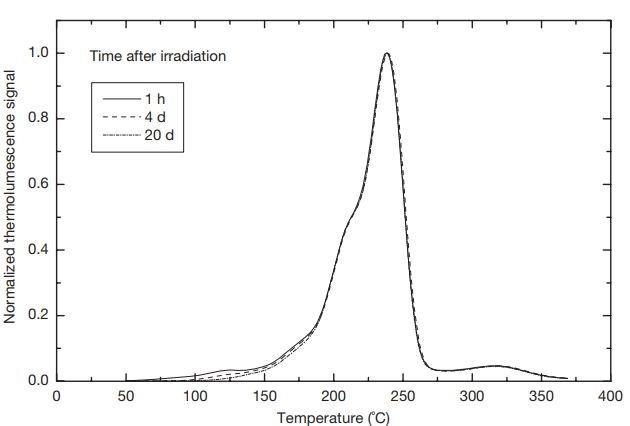
\includegraphics[width=0.5\textwidth]{Imagens/curvLiF.JPG}
		}%
		\caption{Um termograma típico (curva de luminescência) de LiF:Mg,Ti medido com um leitor TLD a uma baixa taxa de aquecimento.}
		\label{fig:curvLiF}
	\end{figure}

	\begin{tcolorbox}[width=\textwidth, colback={white}, colbacktitle={DarkTurquoise!50!white}, title={$\bigstar$ \LobsterTwo{Materiais TLD} $\bigstar$}, coltitle={CarnationPink}, colframe={DarkTurquoise}, fonttitle=\rmfamily\bfseries\Large, breakable]
		\begin{itemize}[label=\textcolor{CarnationPink}{$\star$}]
			\item \textcolor{DarkTurquoise}{\textbf{\ce{LiF}:\ce{Mg}, \ce{Ti}}} \textcolor{MediumOrchid}{\textit{\textbf{(Fluoreto de Lítio dopado com Magnésio e Titânio)}}}: É o material termoluminescente mais amplamente utilizado. Ele possui uma resposta linear com a dose e é eficiente para uma ampla faixa de energias de radiação.
			
			\item \textcolor{DarkTurquoise}{\textbf{\ce{LiF}:\ce{Mg}, \ce{Cu}, \ce{P}}} \textcolor{MediumOrchid}{\textit{\textbf{(Fluoreto de Lítio dopado com Magnésio, Cobre e Fósforo)}}}: Esse material possui uma resposta de dose mais sensível para radiações de baixa energia, tornando-o adequado para monitorar radiação de raios-X de baixa energia como os utilizados em radiodiagnóstico.
			
			\item \textcolor{DarkTurquoise}{\textbf{\ce{Li2B4O7}:\ce{Cu}}} \textcolor{MediumOrchid}{\textit{\textbf{(Borato de lítio dopado com cobre)}}}: Esse material é utilizado em dosímetros termoluminescentes para monitorar doses de radiação gama e raios X.
			
			\item \textcolor{DarkTurquoise}{\textbf{\ce{CaSO4}:\ce{Dy}}} \textcolor{MediumOrchid}{\textit{\textbf{(Sulfato de Cálcio dopado com Disprósio)}}}: Esse material é usado principalmente para monitorar radiação de raios-X em baixas doses.			
			\item \textcolor{DarkTurquoise}{\textbf{\ce{CaF2}:\ce{Dy}}} \textcolor{MediumOrchid}{\textit{\textbf{(Fluoreto de Cálcio dopado com Disprósio)}}}: É adequado para monitorar a dose de radiação devido à feixes de elétrons.			
			\item \textcolor{DarkTurquoise}{\textbf{\ce{CaF2}:\ce{Mn}}} \textcolor{MediumOrchid}{\textit{\textbf{(Fluoreto de cálcio dopado com manganês)}}}: É usado em dosímetros termoluminescentes para medição de doses devido a radiação gama.			
			\item \textcolor{DarkTurquoise}{\textbf{\ce{CaPO4}:\ce{Tl}}} \textcolor{MediumOrchid}{\textit{\textbf{(Fosfato de Cálcio dopado com Tálio)}}}: Também chamado de \textcolor{MediumOrchid}{\textit{\textbf{TLD-100}}} é um dos materiais mais amplamente utilizados na fabricação de dosímetros termoluminescentes devido à sua alta sensibilidade e estabilidade. Ele possui uma resposta termoluminescente linear e é eficiente em uma ampla faixa de energias de radiação, tornando-o adequado para diversas aplicações.			
			\item \textcolor{DarkTurquoise}{\textbf{\ce{MgB4O7}:\ce{Dy}}} \textcolor{MediumOrchid}{\textit{\textbf{(Borato de magnésio dopado com disprósio)}}}: Este material é utilizado em dosímetros termoluminescentes para monitorar doses de radiação gama e raios X.
		\end{itemize}
	\end{tcolorbox}

	Esses materiais termoluminescentes são incorporados em pequenos cristais ou pastilhas que são colocados dentro dos dosímetros TLD. É importante ressaltar que os dosímetros TLD precisam ser calibrados para cada tipo de radiação e faixa de energia específica para garantir medições precisas e confiáveis de doses de radiação.

		% Os dosímetros TLD (Termoluminescent Dosimeters) são dispositivos utilizados para medir a dose de radiação ionizante. Eles são amplamente usados em aplicações de monitoramento de radiação, como proteção radiológica, controle de qualidade em radioterapia e monitoramento de exposição ocupacional.

		% O funcionamento dos dosímetros TLD baseia-se no fenômeno da termoluminescência que é explicado pela teoria de bandas. A teoria de bandas descreve a estrutura eletrônica dos materiais sólidos em termos das energias permitidas para os elétrons e as bandas de energia disponíveis para eles.

		% De acordo com a teoria de bandas, os átomos em um sólido formam uma estrutura cristalina que influencia a distribuição das energias dos elétrons. A estrutura cristalina do material determina as bandas de energia permitidas, que são faixas contínuas de energia eletrônica e as bandas proibidas, que são regiões que não contém níveis de energia permitidos para determinado sólido.
		
		% Quando um material é exposto à radiação ionizante, a energia da radiação é absorvida pelos átomos do material, excitando elétrons de níveis de energia mais baixos (banda de valência) para níveis de energia mais altos. Esses elétrons excitados ocupam temporariamente estados de energia mais altos na banda de condução.
		
		% No entanto, esses elétrons excitados não podem permanecer nos estados de energia excitados por um longo tempo, pois há uma tendência para que eles retornem aos níveis de energia mais baixos. Durante o processo de retorno aos níveis de energia mais baixos, os elétrons liberam a energia armazenada na forma de fótons (luz) na região do espectro eletromagnético visível ou invisível (dependendo do material).
		
		% Porém, quando um material possui impurezas em sua rede cristalina, quando os elétrons retornam para um estado de menor energia eles ficam presos nas armadilhas contidas nas estruturas cristalinas do material chamada de banda proibida. Essa energia armazenada é liberada na forma de luz quando o material é aquecido.
	
	Em resumo, o processo de Dosimetria utilizando o TLD se dá através dos seguintes passos:

		\begin{enumerate}
			\item \textcolor{DarkTurquoise}{\textbf{Exposição à radiação:}} O dosímetro TLD é exposto à radiação ionizante. Durante a exposição, os elétrons dos átomos do material do dosímetro são excitados e ao retornar para o estado fundamental ficam presos nas armadilhas na rede cristalina do material, que possuem um estado de energia superior ao estado fundamental.
			\item \textcolor{DarkTurquoise}{\textbf{Leitura térmica:}} Após a exposição à radiação, o dosímetro é aquecido a uma temperatura adequada, geralmente usando um equipamento chamado leitor de TLD. O aquecimento causa a liberação da energia armazenada na forma de luz visível.
			\item \textcolor{DarkTurquoise}{\textbf{Detecção da luz:}} A luz emitida é detectada por um fotomultiplicador ou um dispositivo semelhante. O sinal de luz é convertido em um sinal elétrico proporcional à quantidade de energia armazenada no dosímetro.
			\item \textcolor{DarkTurquoise}{\textbf{Calibração e análise:}} O sinal elétrico é calibrado em termos de dose de radiação e, em seguida, é analisado para determinar a quantidade de radiação absorvida pelo dosímetro.
		\end{enumerate}
		
		\begin{tcolorbox}[width=\textwidth, colback={white}, colbacktitle={DarkTurquoise!50!white}, title={$\bigstar$ \LobsterTwo{TLD} $\bigstar$}, coltitle={CarnationPink}, colframe={DarkTurquoise}, fonttitle=\rmfamily\bfseries\Large, breakable]

		\textcolor{MediumOrchid}{\Large\LobsterTwo\textbf{Vantagens:}}
		\begin{itemize}[label=\textcolor{CarnationPink}{$\blacktriangleright$}]
			\item \textcolor{DarkTurquoise}{\textbf{Sensibilidade e resposta resposta linear com a dose:}} Os dosímetros TLD possuem uma resposta com a dose relativamente linear, o que significa que sua leitura é proporcional à dose de radiação recebida. Isso os torna adequados para uma ampla faixa de energias de radiação;
			\item \textcolor{DarkTurquoise}{\textbf{Reutilização:}} Os dosímetros TLD podem ser reutilizados após a leitura, tornando-os econômicos a longo prazo. Portanto eles podem ser reaquecidos para zerar possíveis sinalizações térmicas e, em seguida, estar pronto para uma nova exposição à radiação.
			\item \textcolor{DarkTurquoise}{\textbf{Pequeno tamanho e não eletrônico:}} Os dosímetros TLD são compactos e não requerem energia elétrica para operar. Isso os torna fáceis de transportar e usar em diferentes ambientes, além de serem mais seguros por não ser necessário aplicar uma tensão para utilização;
			\item \textcolor{DarkTurquoise}{\textbf{Alta estabilidade a longo prazo:}} Os dosímetros TLD têm boa estabilidade a longo prazo, o que significa que a resposta deles não se deteriora significativamente ao longo do tempo.
		\end{itemize}

		\

		\textcolor{MediumOrchid}{\Large\LobsterTwo\textbf{Desvantagens:}}
		
		\begin{itemize}[label=\textcolor{CarnationPink}{$\blacktriangleright$}]
			\item \textcolor{DarkTurquoise}{\textbf{Leitura demorada:}} A leitura dos dosímetros TLD envolve aquecimento e resfriamento, o que pode levar algumas horas para ser concluído. Isso pode resultar em atrasos na obtenção dos resultados das medições quando precisam ser determinados com certa urgência;
			\item \textcolor{DarkTurquoise}{\textbf{Perda de informação após Leitura:}} Uma vez realizado o aquecimento, a informação é perdida não sendo possível uma releitura;
			\item \textcolor{DarkTurquoise}{\textbf{Sensibilidade à umidade e temperatura:}} Os dosímetros TLD podem ser sensíveis à umidade e temperatura durante o armazenamento, o que pode afetar sua resposta e precisão. Portanto é necessário armazená-los corretamente para evitar esses problemas;
			\item \textcolor{DarkTurquoise}{\textbf{Limitação na leitura em tempo real:}} Embora sejam muito utilizados em dosimetria in vivo, ao contrário de alguns outros tipos de dosímetros, como os dosímetros de estado sólido, os dosímetros TLD não fornecem leituras em tempo real. Isso significa que a dose de radiação não pode ser verificada imediatamente durante a exposição;
			\item \textcolor{DarkTurquoise}{\textbf{Necessidade de equipamento especializado:}} A leitura dos dosímetros TLD requer um leitor de TLD, que é um equipamento especializado. Isso pode representar uma limitação em termos de disponibilidade e custo do equipamento o que pode afetar na escolha deste detector para a rotina clínica.
		\end{itemize}

		\end{tcolorbox}
		
		\

		O tempo necessário para a leitura de um dosímetro TLD pode variar dependendo do tipo específico de dosímetro TLD e das características do equipamento de leitura utilizado. No entanto, geralmente é recomendado aguardar um período de tempo chamado de \textcolor{MediumOrchid}{\textit{\textbf{"período de estabilização"}}} antes de realizar a leitura do dosímetro TLD. Esse período de estabilização é necessário porque os \textcolor{MediumOrchid}{\textit{\textbf{elétrons e íons gerados pela radiação no cristal}}} continuam a \textcolor{MediumOrchid}{\textit{\textbf{interagir com as armadilhas de armazenamento de energia}}} no material termoluminescente do dosímetro TLD mesmo \textcolor{MediumOrchid}{\textit{\textbf{após a exposição à radiação ter sido encerrada}}}. Essa interação pode resultar em uma resposta termoluminescente adicional, chamada de \textcolor{MediumOrchid}{\textit{\textbf{"autoextinção" }}}(também conhecida como autoextinguishing ou fading), que pode afetar a leitura correta da dose de radiação. 

		Em geral, \textcolor{MediumOrchid}{\textit{\textbf{é comum aguardar pelo menos algumas horas, e até mesmo algumas dezenas de horas (cerca de 24h), antes de realizar a leitura de um dosímetro TLD}}}. O tempo exato necessário para o período de estabilização pode ser determinado pelo fabricante do dosímetro TLD ou pelas diretrizes e procedimentos específicos adotados pelo laboratório ou serviço de dosimetria.

		\begin{figure}[h]
			\centering
			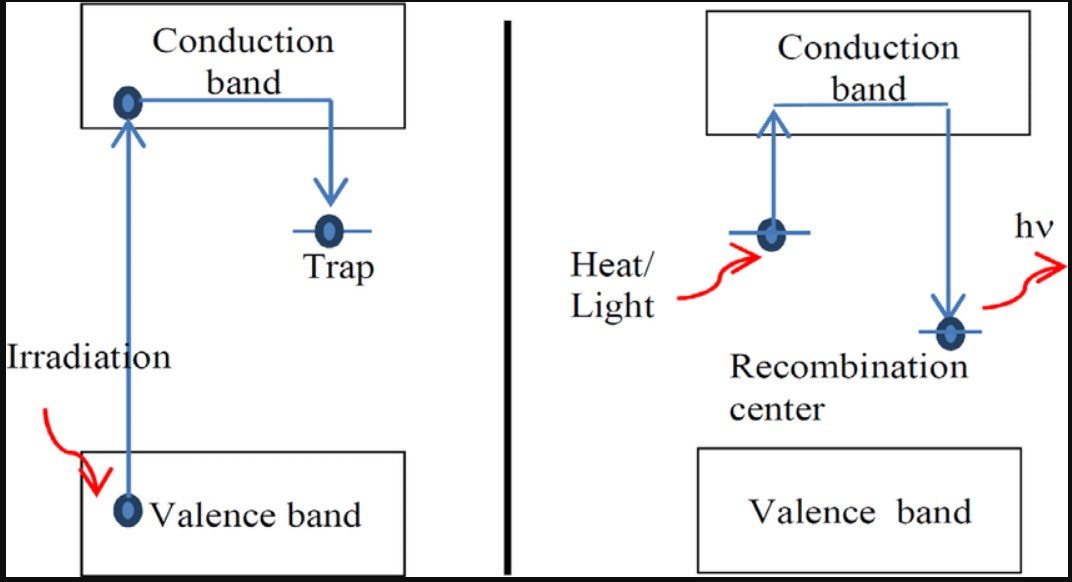
\includegraphics[width=0.5\textwidth]{Imagens/tldOsld.jpg}
			\caption{Exemplo da teoria de bandas nos fenômenos de termoluminescência (TLD - Aquecimento) e luminescência Opticamente estimulada (OSLD - Luz)}
			\label{fig:tldOsld}
		\end{figure}

\subsubsection*{Dosímetros Luminescentes Opticamente Estimulados (OSLD)}

	A luminescência estimulada opticamente (OSL) é uma técnica de dosimetria que utiliza luz, especificamente luz laser, para liberar a energia aprisionada em armadilhas de um material luminescente. 

	O dosímetro de OSL consiste em um pequeno chip feito de \textcolor{MediumOrchid}{\textit{\textbf{óxido de alumínio dopado com carbono (\ce{Al2O3}:\ce{C})}}}, com tamanho aproximado de 1 \unit{mm^3}. Esse chip é acoplado a uma \textcolor{MediumOrchid}{\textit{\textbf{fibra óptica}}}. O sistema de dosímetro também inclui um \textcolor{MediumOrchid}{\textit{\textbf{laser, um divisor de feixe, um colimador, um tubo fotomultiplicador (PMT), eletrônicos e software}}}. No sistema, o chip é excitado com luz laser por meio da fibra óptica, e a luminescência resultante (luz azul) é coletada de volta através da mesma fibra óptica, refletida pelo divisor de feixe em um ângulo de \ang{90} e medida pelo PMT.

	O dosímetro de OSL possui \textcolor{MediumOrchid}{\textit{\textbf{alta sensibilidade em uma ampla faixa de taxas de dose e doses}}} utilizadas em radioterapia. Sua resposta é geralmente \textcolor{MediumOrchid}{\textit{\textbf{linear}}} e \textcolor{MediumOrchid}{\textit{\textbf{independente de energia e taxa de dose}}}. Isso significa que o sinal de OSL é proporcional à dose absorvida, independentemente da energia da radiação e da taxa de dose aplicada. No entanto, podem ser necessárias correções para levar em consideração a \textcolor{MediumOrchid}{\textit{\textbf{resposta angular do dosímetro}}}, ou seja, a dependência da resposta em relação à direção de incidência da radiação.

	Além da configuração básica de OSL, existem outras configurações experimentais possíveis. Uma delas é a \textcolor{MediumOrchid}{\textit{\textbf{OSL pulsada}}}, na qual o dosímetro é estimulado com pulsos de luz laser em vez de uma exposição contínua. Essa técnica pode fornecer \textcolor{MediumOrchid}{\textit{\textbf{informações adicionais sobre a taxa de dose}}} durante a irradiação. Outra configuração é a combinação da OSL com a \textcolor{MediumOrchid}{\textit{\textbf{radioluminescência}}}, que é a emissão de luz \textcolor{MediumOrchid}{\textit{\textbf{imediata}}} pelo dosímetro durante a irradiação. A radioluminescência fornece uma \textcolor{MediumOrchid}{\textit{\textbf{resposta em tempo real}}} da dose durante o tratamento, enquanto a OSL fornece a \textcolor{MediumOrchid}{\textit{\textbf{dose integral}}} posteriormente.


		% Os dosímetros OSLD (Optically Stimulated Luminescence Dosimeters) funcionam com base no fenômeno da luminescência estimulada opticamente. 

		% Quando o dosímetro é exposto à radiação ionizante, ocorre a interação entre a radiação e os átomos do cristal, gerando íons e elétrons livres. Alguns dos elétrons livres ficam presos nas armadilhas eletrônicas do material sensível à radiação. Após a exposição à radiação, o dosímetro é colocado em um leitor de OSLD. Durante a leitura, o dosímetro é iluminado com uma luz de estimulação, geralmente na faixa de comprimento de onda ultravioleta ou visível. A luz de estimulação libera os elétrons presos nas armadilhas eletrônicas, fazendo com que retornem aos seus estados de energia mais baixos. À medida que os elétrons retornam aos seus estados de energia mais baixos, eles emitem luz na forma de luminescência. Essa luminescência é medida pelo leitor de OSLD, que converte o sinal óptico em um sinal elétrico proporcional à dose de radiação recebida pelo dosímetro. A intensidade da luminescência é proporcional à quantidade de radiação absorvida pelo dosímetro. O leitor de OSLD registra essa intensidade luminescente e calcula a dose de radiação com base em calibrações prévias, que relacionam a intensidade luminescente com a dose de radiação. A tecnologia OSLD é usada em serviços de dosimetria de radiações ionizantes por raios-x, gama e beta. Também pode ser empregada para detecção de nêutrons, embora este uso não seja praticado ainda no Brasil.

	\begin{tcolorbox}[width=\textwidth, colback={white}, colbacktitle={DarkTurquoise!50!white}, title={$\bigstar$ \LobsterTwo{Materiais OSL} $\bigstar$}, coltitle={CarnationPink}, colframe={DarkTurquoise}, fonttitle=\rmfamily\bfseries\Large, breakable]
		\begin{itemize}[label=\textcolor{CarnationPink}{$\star$}]
			\item \textcolor{DarkTurquoise}{\textbf{\ce{Al2O3}:\ce{C}}} \textcolor{MediumOrchid}{\textit{\textbf{(Óxido de Alumínio dopado com Carbono)}}}: Emite uma luminescencia de $420 \text{ nm}$ quando é estimulado com uma luz de $540 \text{ nm}.$
			\item \textcolor{DarkTurquoise}{\textbf{\ce{Al2O3}:\ce{C}, \ce{Mg}}} \textcolor{MediumOrchid}{\textit{\textbf{(Óxido de Alumíno dopado com Carbono e Magnésio)}}}
			\item O \textcolor{DarkTurquoise}{\textbf{\ce{Al2O3}}} também pode ser dopado com elementos terras raras como o \textcolor{DarkTurquoise}{\ce{Ce}} (cério) e o \textcolor{DarkTurquoise}{\ce{Tl}} (tálio).
		\end{itemize}
	\end{tcolorbox}

	


	\begin{tcolorbox}[width=\textwidth, colback={white}, colbacktitle={DarkTurquoise!50!white}, title={$\bigstar$ \LobsterTwo{Dosímetros OSL} $\bigstar$}, coltitle={CarnationPink}, colframe={DarkTurquoise}, fonttitle=\rmfamily\bfseries\Large, breakable]

	\textcolor{MediumOrchid}{\Large\LobsterTwo\textbf{Vantagens:}}
	\begin{itemize}[label=\textcolor{CarnationPink}{$\blacktriangleright$}]
		\item \textcolor{DarkTurquoise}{\textbf{Alta sensibilidade:}} Os dosímetros OSL são altamente sensíveis à radiação ionizante, permitindo a detecção e medição precisa de doses de radiação relativamente baixas. Isso é especialmente importante em áreas onde doses baixas são relevantes, como medicina nuclear e dose espalhada em radioterapia.
		\item \textcolor{DarkTurquoise}{\textbf{Ampla faixa de dose absorvida:}} Os dosímetros OSL podem cobrir uma ampla faixa de dose de radiação, desde doses muito baixas até doses muito altas. Isso os torna adequados para diferentes aplicações, desde monitoramento de exposição ocupacional até medição de doses terapêuticas em radioterapia.
		\item \textcolor{DarkTurquoise}{\textbf{Estabilidade a longo prazo:}} Os dosímetros OSL têm uma estabilidade a longo prazo em relação à resposta luminosa. Isso significa que eles mantêm sua calibração e resposta ao longo do tempo, o que é essencial para garantir medições confiáveis e consistentes ao longo de períodos prolongados.
		\item \textcolor{DarkTurquoise}{\textbf{Re-leitura:}} A capacidade de obter medições precisas e rápidas da dose integrada logo após a irradiação é uma vantagem significativa, permitindo uma avaliação mais imediata e precisa da dose entregue ao paciente. Uma característica dos OSLDs é a possibilidade de arquivamento do dosímetro e a verificação da dose por meio de \textcolor{MediumOrchid}{\textit{\textbf{leitura não-destrutiva}}}, o que torna possível a reanálise completa das amostras e a realização de avaliações incrementais para rastreamento da exposição ao longo do tempo.
	\end{itemize}

	\textcolor{MediumOrchid}{\Large\LobsterTwo\textbf{Desvantagens:}}
	\begin{itemize}[label=\textcolor{CarnationPink}{$\blacktriangleright$}]
		\item \textcolor{DarkTurquoise}{\textbf{Sensibilidade à luz ambiente:}} Os dosímetros OSL podem ser sensíveis à luz ambiente. Isso significa que a exposição à luz antes da leitura pode afetar a resposta do dosímetro, levando a resultados imprecisos. Portanto, é necessário tomar precauções para proteger o dosímetro da luz não intencional.
		\item \textcolor{DarkTurquoise}{\textbf{Complexidade da leitura:}} A leitura dos dosímetros OSL requer equipamentos específicos, como leitores de OSL, que nem sempre estão disponíveis em todos os locais. Isso pode limitar a capacidade de leitura imediata em algumas situações e exigir a transferência dos dosímetros para um local apropriado para a leitura.
		\item \textcolor{DarkTurquoise}{\textbf{Sensibilidade a altas temperaturas:}} Os dosímetros OSL podem ser sensíveis a altas temperaturas. Exposição a temperaturas elevadas pode levar a alterações na resposta do dosímetro e afetar a precisão das medições. É importante armazenar e manusear os dosímetros dentro dos limites de temperatura recomendados pelo fabricante.
		\item \textcolor{DarkTurquoise}{\textbf{Dependência com o tipo de radiação:}} A resposta dos dosímetros OSL pode variar dependendo do tipo de radiação ionizante. Eles podem ter diferentes eficiências de detecção para diferentes tipos de partículas (como fótons, elétrons ou nêutrons). Portanto, a resposta do dosímetro OSL pode não ser igual para todos os tipos de radiação, exigindo fatores de correção ou ajustes para diferentes tipos de exposição.
	\end{itemize}
	\end{tcolorbox}

\subsection*{Detectores de Estado Sólido -- Dosímetros Semicondutores}

Os detectores de radiação de estado sólido, também conhecidos como diodos detectores de radiação, são dispositivos semicondutores que são sensíveis à radiação ionizante. Eles são amplamente utilizados para detectar e medir a radiação em diversas aplicações, como medicina nuclear, radioterapia, monitoramento ambiental e segurança nuclear.

	\begin{tcolorbox}[width=\textwidth, colback={white}, colbacktitle={DarkTurquoise!50!white}, title={$\bigstar$ \LobsterTwo{Principais Materiais: Diodos} $\bigstar$}, coltitle={CarnationPink}, colframe={DarkTurquoise}, fonttitle=\rmfamily\bfseries\Large, breakable]
	\begin{itemize}[label=\textcolor{CarnationPink}{$\star$}]
		\item \textcolor{DarkTurquoise}{\textbf{Silício (\ce{Si}):}} O silício é o material semicondutor mais amplamente utilizado na indústria eletrônica. É abundante, possui um intervalo de energia adequado e pode ser facilmente dopado para criar diodos com diferentes características. É bastante sensível à radiação ionizante, especialmente para detectar radiação de partículas alfa. O silício pode ser dopado com átomos de \textcolor{MediumOrchid}{\textit{\textbf{fósforo (P)}}} para criar o semicondutor \textcolor{MediumOrchid}{\textit{\textbf{tipo n}}} adicionando elétrons extras, ou com átomos de \textcolor{MediumOrchid}{\textit{\textbf{boro (B)}}} para criar o semicondutor \textcolor{MediumOrchid}{\textit{\textbf{tipo p}}}, adicionando buracos.
				
		\item \textcolor{DarkTurquoise}{\textbf{Germânio (\ce{Ge}):}} O germânio é um material semicondutor que apresenta maior eficiência na detecção de radiação ionizante em comparação ao silício. É frequentemente usado em detectores de radiação de alta energia, como a espectrometria de raios X.  O germânio pode ser dopado de maneira semelhante ao silício, utilizando átomos de fósforo para criar o tipo n e átomos de boro para criar o tipo p.
				
		\item \textcolor{DarkTurquoise}{\textbf{Telureto de cádmio (\ce{CdTe}):}} O telureto de cádmio é um material semicondutor composto usado em detectores de radiação de alta eficiência, especialmente para detecção de raios X e gama. É dopado com impurezas de cádmio (Cd) e telúrio (Te) para ajustar suas propriedades elétricas.

		\item \textcolor{DarkTurquoise}{\textbf{Telureto de cádmio-zinco (\ce{CdZnTe}):}} O CdZnTe é outro material semicondutor composto usado em detectores de radiação, especialmente para aplicações de detecção de raios X e gama. Ele é dopado com impurezas de cádmio (Cd) e zinco (Zn).
	\end{itemize}
	\end{tcolorbox}

\subsubsection*{Diodos de Silício}

	Um dosímetro com diodo de silício é baseado em uma \textcolor{MediumOrchid}{\textit{\textbf{estrutura de diodo de junção p-n}}}, onde o silício é dopado para criar uma região de tipo n ou tipo p, e a superfície é dopada de maneira contrária para criar o tipo oposto de material. Os diodos são comumente chamados de dosímetros n-Si ou p-Si, dependendo do material base. Entre os dois tipos, o p-Si é mais adequado para dosimetria em radioterapia devido à sua menor suscetibilidade a danos por radiação e corrente escura mais baixa.

	Quando a radiação interage com o dosímetro de diodo de silício, \textcolor{MediumOrchid}{\textit{\textbf{pares elétron-buraco (e-h)}}} são gerados dentro do \textcolor{MediumOrchid}{\textit{\textbf{corpo do diodo}}}, incluindo a \textcolor{MediumOrchid}{\textit{\textbf{região de depleção}}}. Essas cargas geradas dentro do comprimento de difusão do dosímetro difundem-se para a região de depleção. Em seguida, são varridas através dessa região pelo \textcolor{MediumOrchid}{\textit{\textbf{campo elétrico gerado pelo potencial intrínseco}}}. Esse processo resulta na geração de uma \textcolor{MediumOrchid}{\textit{\textbf{corrente reversa}}} no diodo. A magnitude da corrente reversa está relacionada à dose absorvida.

	A resposta dos dosímetros de diodo de silício é tipicamente \textcolor{MediumOrchid}{\textit{\textbf{linear}}} e \textcolor{MediumOrchid}{\textit{\textbf{independente da energia}}} dentro da faixa de energia terapêutica. Isso significa que a relação entre a corrente reversa e a dose absorvida é proporcional e não depende do tipo de radiação utilizada para a irradiação. Essa característica é vantajosa, pois permite uma dosimetria precisa independentemente da energia do feixe de radiação utilizado.

	Os dosímetros de diodo de silício oferecem vantagens significativas, como \textcolor{MediumOrchid}{\textit{\textbf{tamanho reduzido}}}, \textcolor{MediumOrchid}{\textit{\textbf{equivalência ao tecido humano}}}, \textcolor{MediumOrchid}{\textit{\textbf{alta resolução espacial}}} e \textcolor{MediumOrchid}{\textit{\textbf{medição de dose em tempo real}}}. Devido ao seu tamanho compacto, os diodos de silício podem ser facilmente posicionados em locais críticos para medir a dose com alta precisão. Sua equivalência ao tecido humano é importante, pois a resposta do dosímetro se assemelha à resposta dos tecidos humanos à radiação. Além disso, a capacidade de medir a dose em tempo real permite o monitoramento contínuo da dose durante o tratamento.

	Os dosímetros de diodo de silício são amplamente utilizados em radioterapia para diversas aplicações. Eles são empregados na \textcolor{MediumOrchid}{\textit{\textbf{dosimetria in vivo}}}, permitindo a medição direta da dose absorvida pelo paciente durante o tratamento. Também são utilizados no \textcolor{MediumOrchid}{\textit{\textbf{comissionamento do feixe}}}, \textcolor{MediumOrchid}{\textit{\textbf{garantia de qualidade}}} e \textcolor{MediumOrchid}{\textit{\textbf{verificação da dose específica do paciente}}}, garantindo que o plano de tratamento esteja sendo entregue corretamente. Sua alta resolução espacial e resposta em tempo real os tornam uma escolha valiosa em várias etapas do processo de radioterapia.

	\begin{exemplo}[Pontos Importantes sobre o Diodo de Silício]
		\begin{itemize}
			\item \textcolor{DarkTurquoise}{\textbf{Os diodos de silício são operados no modo de curto-circuito}}, o que significa que não é aplicado bias externo para reduzir a corrente de fuga. Essa configuração fornece uma relação linear entre a carga medida e a dose absorvida. O curto-circuito também evita a polarização do diodo, permitindo uma resposta direta à radiação incidente.
			\item \textcolor{DarkTurquoise}{\textbf{Em comparação com câmaras de ionização, os diodos de silício são mais sensíveis e menores em tamanho}}. Sua alta sensibilidade os torna capazes de medir doses menores com precisão, enquanto seu tamanho compacto permite que sejam posicionados em regiões de interesse com alta resolução espacial. No entanto, é importante destacar que os diodos de silício são dosímetros relativos e não devem ser usados para calibração do feixe devido à sensibilidade que pode variar com o uso repetido, causado por danos por radiação.
			\item \textcolor{DarkTurquoise}{\textbf{Os diodos de silício são particularmente úteis para medições em fantomas, como pequenos campos em radiocirurgia estereotáxica ou regiões com alto gradiente de dose, como a penumbra}}. Sua capacidade de medir diretamente a distribuição de dose os torna valiosos em áreas onde as câmaras de ionização podem ter dificuldade devido ao seu tamanho maior. Além disso, os diodos são comumente utilizados para medições de dose em profundidade em feixes de elétrons. Quando usados em combinação com dispositivos de varredura do feixe em fantomas de água, os diodos são encapsulados à prova d'água para proteção.
			\item \textcolor{DarkTurquoise}{\textbf{Os diodos de silício são amplamente utilizados na dosimetria in vivo de rotina em pacientes}}. Eles são frequentemente usados para medições de dose na bexiga ou no reto durante tratamentos de radioterapia. Para a dosimetria in vivo, os diodos são equipados com encapsulamento de acumulação, que oferece proteção física ao diodo e requer seleção adequada com base no tipo e qualidade dos feixes clínicos.
			\item \textcolor{DarkTurquoise}{\textbf{A calibração é necessária ao usar diodos de silício para dosimetria in vivo}}. É importante aplicar vários fatores de correção para calcular com precisão a dose absorvida. A sensibilidade dos diodos pode variar devido ao histórico de radiação, portanto, recalibrações periódicas são necessárias para manter a precisão das medições.
			\item \textcolor{DarkTurquoise}{\textbf{Os diodos de silício apresentam variações na resposta à dose relacionadas à temperatura}}. É especialmente importante considerar essas variações durante tratamentos prolongados de radioterapia. Além disso, os diodos também mostram dependência da taxa de dose, dependência angular e dependência de energia. Essas dependências devem ser levadas em conta ao realizar medições de dose, especialmente em diferentes distâncias fonte-pele e para diferentes energias espectrais dos feixes de radiação. A dependência de energia é particularmente relevante para medir as doses de entrada e saída em tratamentos de radioterapia.
		\end{itemize}
	\end{exemplo}

	\

	\begin{tcolorbox}[width=\textwidth, colback={white}, colbacktitle={DarkTurquoise!50!white}, title={$\bigstar$ \LobsterTwo{Diodos} $\bigstar$}, coltitle={CarnationPink}, colframe={DarkTurquoise}, fonttitle=\rmfamily\bfseries\Large, breakable]
		\textcolor{MediumOrchid}{\Large\LobsterTwo\textbf{Vantagens:}}
		\begin{itemize}[label=\textcolor{CarnationPink}{$\blacktriangleright$}]
			\item \textcolor{DarkTurquoise}{\textbf{Alta sensibilidade:}} Os diodos semicondutores têm uma alta sensibilidade à radiação ionizante, permitindo a detecção de níveis muito baixos de radiação.
			\item \textcolor{DarkTurquoise}{\textbf{Resposta rápida:}} Os diodos semicondutores têm uma resposta rápida à radiação, permitindo uma medição em tempo real da dose de radiação.
			\item \textcolor{DarkTurquoise}{\textbf{Faixa dinâmica ampla:}} Os diodos semicondutores possuem uma ampla faixa dinâmica, o que significa que podem medir uma ampla gama de doses de radiação, desde níveis baixos até níveis muito altos.
			\item \textcolor{DarkTurquoise}{\textbf{Tamanho compacto:}} Os diodos semicondutores são dispositivos pequenos e compactos, o que facilita sua integração em sistemas e equipamentos de detecção.
		\end{itemize}

			
		\textcolor{MediumOrchid}{\Large\LobsterTwo\textbf{Desvantagens:}}
		\begin{itemize}[label=\textcolor{CarnationPink}{$\blacktriangleright$}]
			\item \textcolor{DarkTurquoise}{\textbf{Sensibilidade à temperatura:}} Os diodos semicondutores são sensíveis a variações de temperatura, o que pode afetar sua resposta e precisão na medição da dose de radiação.
			\item \textcolor{DarkTurquoise}{\textbf{Efeito de dano por radiação:}} A exposição prolongada à radiação pode causar danos ao material do diodo, levando a alterações em suas propriedades elétricas e, eventualmente, à falha do dispositivo.
			\item \textcolor{DarkTurquoise}{\textbf{Custo}}: Os diodos semicondutores, especialmente aqueles de alta qualidade e desempenho, podem ser relativamente caros em comparação com outros tipos de detectores de radiação.
			\item \textcolor{DarkTurquoise}{\textbf{Efeito de envelhecimento:}} Com o tempo, os diodos semicondutores podem sofrer degradação de desempenho devido ao envelhecimento, o que pode levar a uma diminuição da sensibilidade e precisão ao longo do tempo.
			\item \textcolor{DarkTurquoise}{\textbf{Efeito da Geometria:}} Este detector tem variabilidade no posicionamento causando uma dependência direcional, possui dependência energética em feixes de fótons.
		\end{itemize}
	\end{tcolorbox}

\subsubsection*{MOSFET}

	Os detectores \textcolor{MediumOrchid}{\textit{\textbf{MOSFETs (Metal-Oxide-Semiconductor Field-Effect Transistors)}}} são dispositivos semicondutores que são amplamente utilizados como detectores de radiação. Eles são baseados na tecnologia dos transistores de efeito de campo (FET) de óxido de metal-semicondutor (MOS). Ele é conhecido por ter uma \textcolor{MediumOrchid}{\textit{\textbf{resolução espacial excepcional}}}, ou seja, é capaz de medir com alta precisão as características de um objeto em termos de \textcolor{MediumOrchid}{\textit{\textbf{posição e tamanho}}}. Além disso, o MOSFET apresenta uma \textcolor{MediumOrchid}{\textit{\textbf{mínima atenuação do feixe de radiação}}}, o que significa que ele não causa uma redução significativa na intensidade do feixe de radiação ao passar por ele.

	\begin{wrapfigure}{r}{0.45\textwidth}
		\centering
		\fcolorbox{DarkTurquoise}{white}{%
			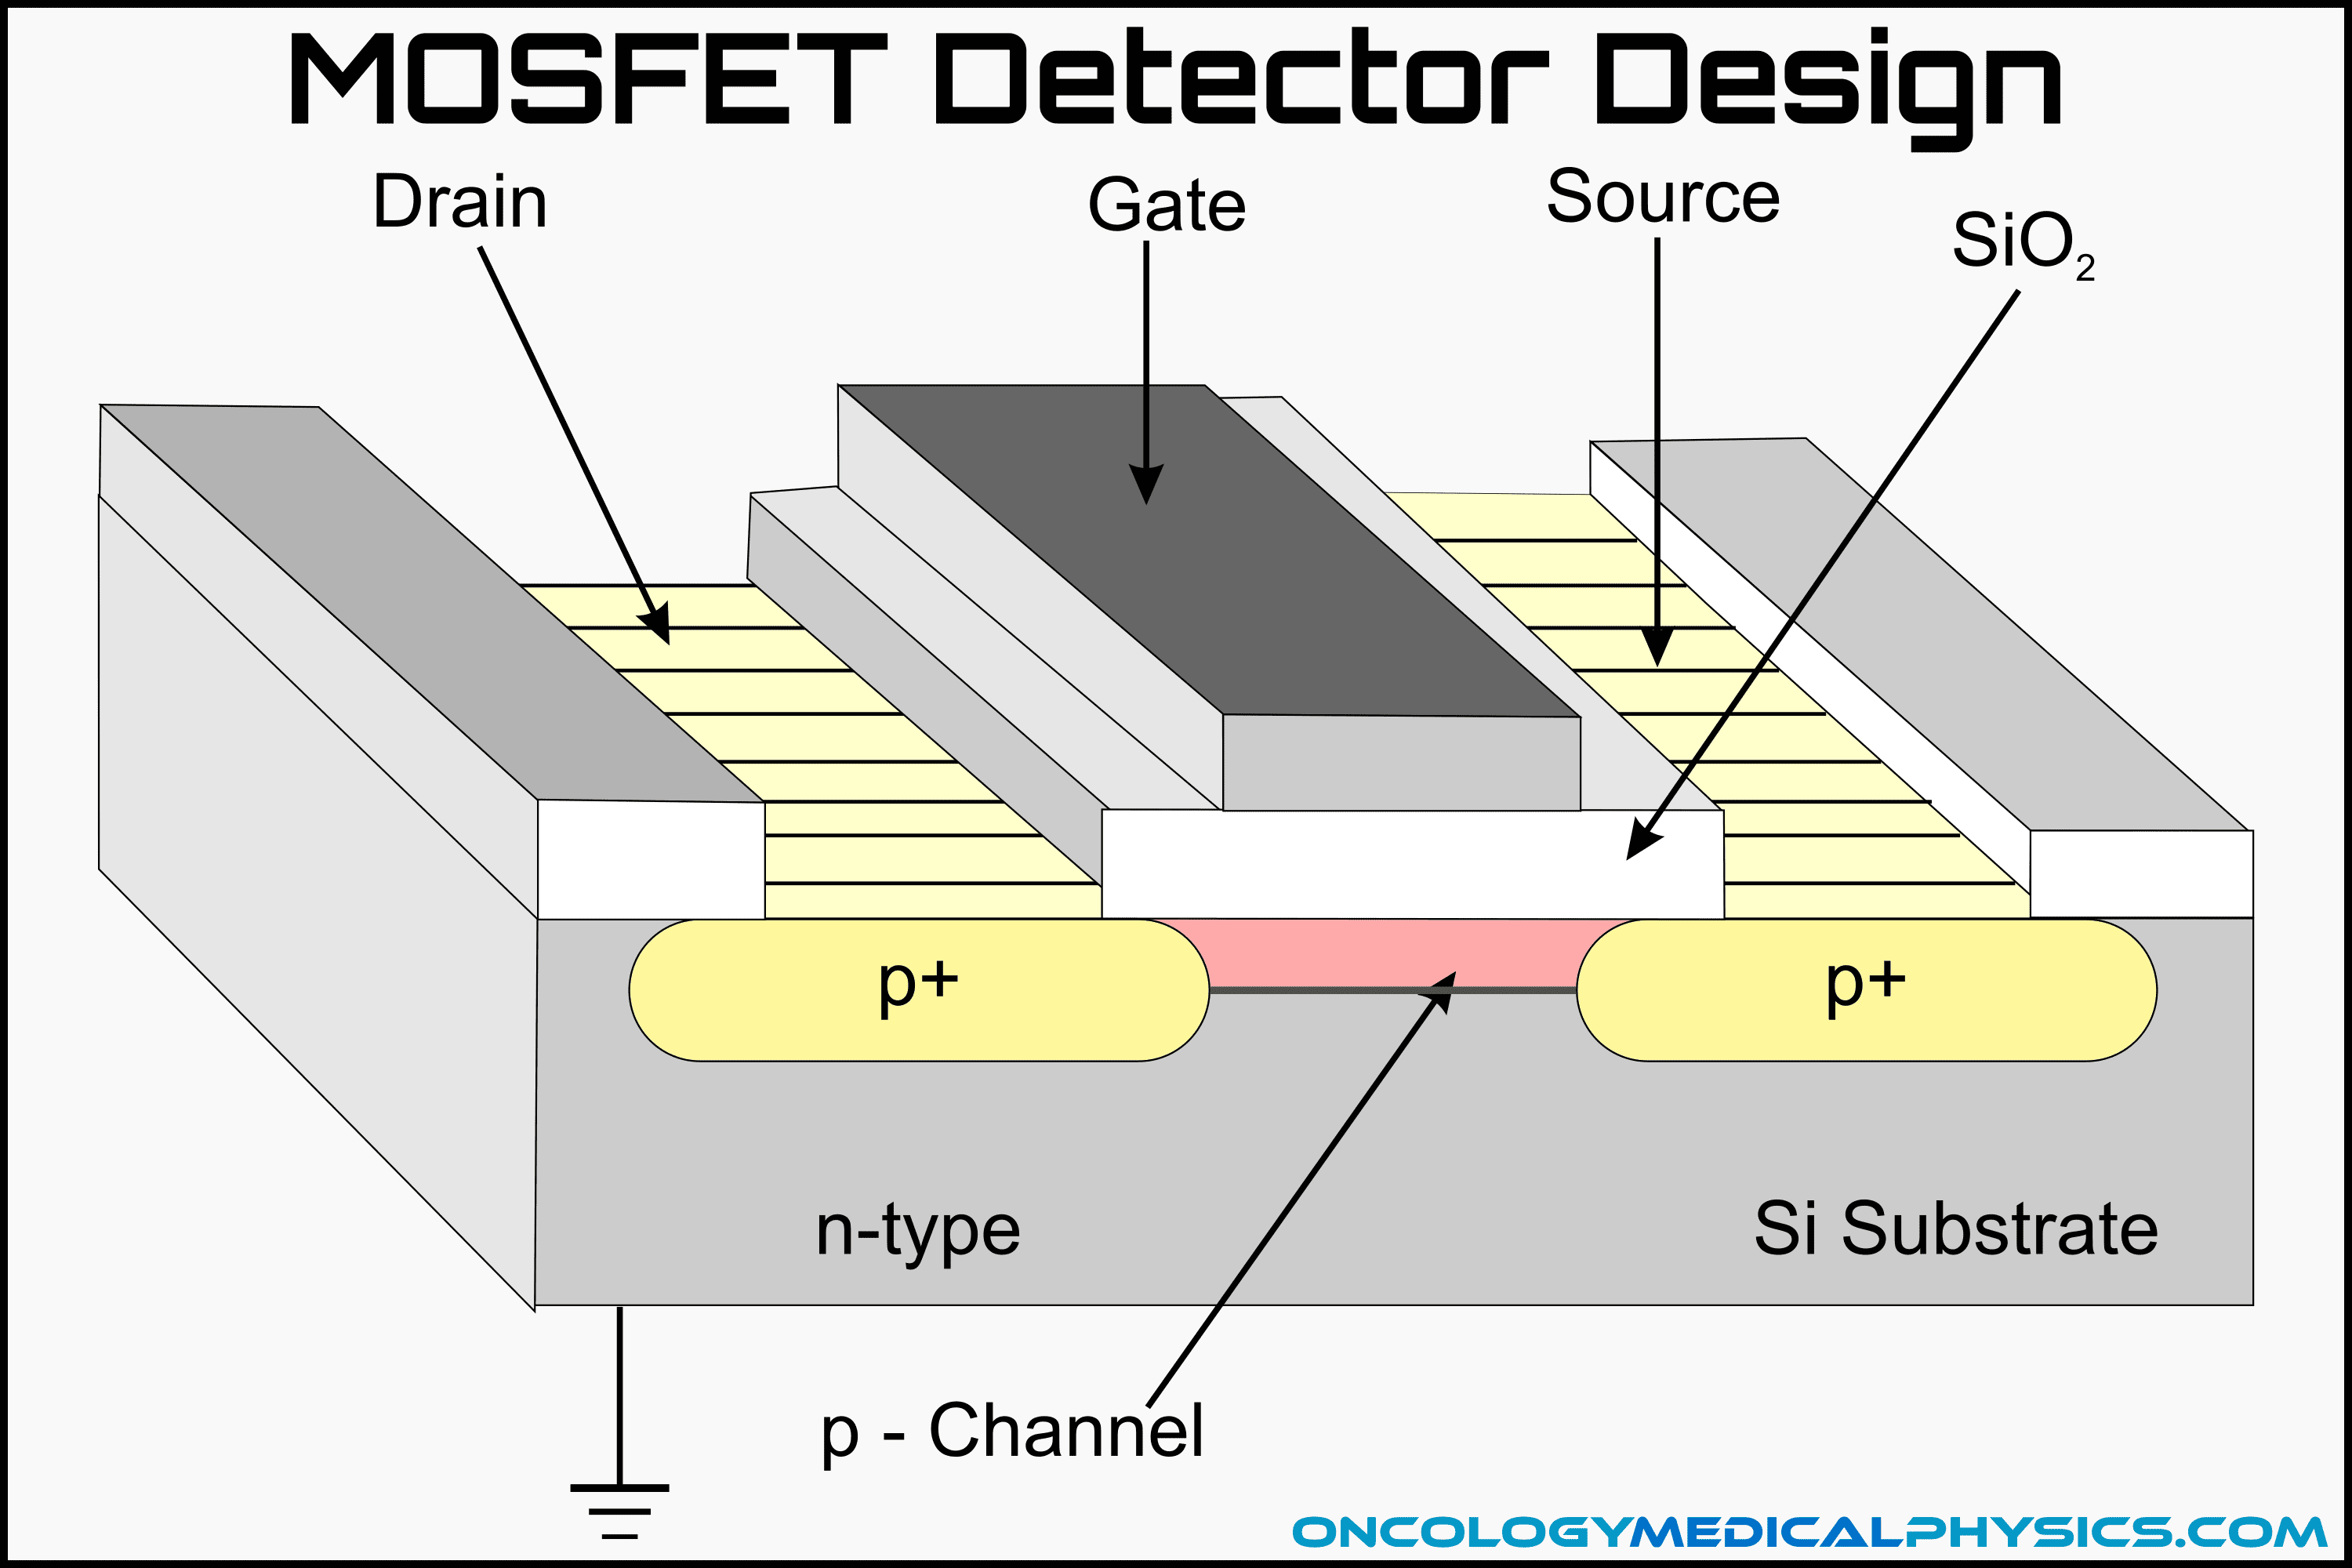
\includegraphics[width=0.40\textwidth]{Imagens/mosfet.png}
		}%
		\caption{Esquema de um MOSFET}
		\label{fig:mosfet}
	\end{wrapfigure}

	Os detectores MOSFET consistem em uma estrutura de três camadas: \textcolor{MediumOrchid}{\textit{\textbf{o substrato semicondutor, o óxido de isolamento e o metal de controle}}} (\ref{fig:mosfet}). O substrato semicondutor é dopado para criar uma região tipo p (p-channel MOSFET) ou tipo n (n-channel MOSFET). O óxido de isolamento é depositado sobre o substrato e atua como um isolante elétrico. O metal de controle é aplicado sobre o óxido de isolamento e funciona como o terminal de controle do transistor.
	
	Quando um MOSFET é irradiado com radiação ionizante, a interação da radiação com o substrato semicondutor gera pares de elétrons e buracos. Esses portadores de carga afetam a condutividade do substrato semicondutor, resultando em uma alteração na corrente elétrica que flui através do MOSFET. Essa alteração na corrente é proporcional à dose de radiação incidente.
	
	Os dosímetros MOSFET operam medindo a \textcolor{MediumOrchid}{\textit{\textbf{tensão de limiar}}}, que é a \textcolor{MediumOrchid}{\textit{\textbf{tensão necessária para que o transistor comece a conduzir corrente}}}. Essa tensão de limiar possui uma relação linear com a dose de radiação absorvida. Quando a radiação ionizante penetra na camada de óxido do MOSFET, ela gera carga que fica aprisionada permanentemente nessa região, causando uma mudança na tensão de limiar. Essa mudança na tensão é proporcional à dose de radiação absorvida. A dose cumulativa, ou seja, a dose total recebida durante um determinado período de tempo, pode ser medida durante ou após a irradiação usando os dosímetros MOSFET.

	Um aspecto importante dos MOSFETs é o fato de que eles \textcolor{MediumOrchid}{\textit{\textbf{requerem uma conexão com uma tensão de polarização constante}}} durante a irradiação para funcionar corretamente. Essa polarização é necessária para garantir a estabilidade e a precisão das medições da dose absorvida. Além disso, é os MOSFETs possuem uma vida útil limitada devido ao envelhecimento do dispositivo e ao acúmulo de carga no óxido ao longo do tempo. Portanto, \textcolor{MediumOrchid}{\textit{\textbf{é necessário realizar verificações periódicas de calibração e substituir os dosímetros quando sua precisão estiver comprometida}}}.

	Os detectores MOSFET possuem várias vantagens, como \textcolor{MediumOrchid}{\textit{\textbf{alta sensibilidade, resposta rápida, faixa dinâmica ampla, boa resolução espacial e baixo consumo de energia}}}. Além disso, eles são \textcolor{MediumOrchid}{\textit{\textbf{reutilizáveis}}} e podem ser facilmente integrados a sistemas de leitura e análise.

	\begin{exemplo}[Pontos Importantes do MOSFET:]
		\begin{itemize}
			\item \textcolor{DarkTurquoise}{\textbf{Um único dosímetro MOSFET pode cobrir toda a faixa de energia de fótons e elétrons}}. Isso significa que o MOSFET é capaz de medir a dose absorvida em diferentes energias de radiação. No entanto, é importante levar em consideração que a resposta do MOSFET pode variar dependendo da qualidade da radiação, ou seja, das características específicas do feixe de radiação. Portanto, é necessário avaliar a resposta do MOSFET em relação à energia utilizada durante a irradiação. No caso de feixes de megavoltagem, que são comumente usados na radioterapia, os MOSFETs geralmente não requerem correções de energia adicionais. Um único fator de calibração pode ser suficiente para esses casos.
			\item \textcolor{DarkTurquoise}{\textbf{Os MOSFETs apresentam uma anisotropia axial mínima}}. A anisotropia refere-se à variação da resposta do dosímetro em diferentes ângulos em relação ao feixe de radiação. A anisotropia axial mínima significa que a resposta do MOSFET varia apenas ligeiramente ($\pm$ 2\%) em torno de uma rotação de \ang{360} em torno de seu eixo. Isso indica uma resposta direcionalmente uniforme do MOSFET. Além disso, os MOSFETs geralmente não requerem correções de taxa de dose, o que significa que a leitura do dosímetro não precisa ser ajustada em relação à taxa de entrega da dose de radiação.
			\item \textcolor{DarkTurquoise}{\textbf{Assim como os diodos utilizados em dosimetria, os MOSFETs também são afetados pela temperatura}}. No entanto, esse problema foi resolvido com o desenvolvimento de sistemas de MOSFETs duplos especialmente projetados, que compensam a dependência da temperatura. Em geral, os MOSFETs podem apresentar uma resposta não linear em relação à dose absorvida total. No entanto, dentro de sua vida útil especificada, eles mantêm uma linearidade satisfatória, ou seja, a resposta do MOSFET é proporcional à dose absorvida de forma previsível.
			\item \textcolor{DarkTurquoise}{\textbf{Os MOSFETs são sensíveis a mudanças na tensão de polarização durante a irradiação}}, o que significa que é importante manter uma tensão estável para garantir a precisão das medições. Também é mencionado que a resposta dos MOSFETs pode sofrer pequenas variações após a irradiação. Portanto, é necessário realizar as leituras do dosímetro dentro de um período de tempo específico após a exposição à radiação para obter resultados precisos e confiáveis.
		\end{itemize}
	\end{exemplo}

\subsection*{Outros Detectores}

\subsubsection*{Cintiladores}

		Os detectores de cintilação, também conhecidos como detectores de cintiladores, são dispositivos que \textcolor{MediumOrchid}{\textit{\textbf{convertem a energia da radiação incidente em luz visível ou infravermelha próxima}}}. Essa conversão ocorre dentro de um material chamado cintilador, que é composto por cristais ou materiais orgânicos.

		Durante a irradiação, esses cintiladores geram luz, que é então transmitida por meio de fibras ópticas para um tubo fotomultiplicador (PMT) localizado fora da sala de irradiação. Em uma configuração típica, são usados dois conjuntos de fibras ópticas conectados a dois PMTs diferentes, permitindo a subtração do sinal de radiação Cerenkov de fundo. A resposta do dosímetro de cintilação é \textcolor{MediumOrchid}{\textit{\textbf{linear}}} dentro da faixa de dose terapêutica de interesse.

		Em termos de densidade eletrônica e composição atômica, \textcolor{MediumOrchid}{\textit{\textbf{os cintiladores de plástico são muito semelhantes à água}}}. Eles geralmente têm uma densidade eletrônica e um coeficiente de absorção de energia de massa que correspondem aproximadamente aos valores da água, com uma variação de $\pm$2\% para a faixa de energias de feixes comumente usados na prática clínica, incluindo a região de kilovoltagem. Os cintiladores de plástico apresentam uma \textcolor{MediumOrchid}{\textit{\textbf{dependência mínima em relação à energia}}}, o que os torna adequados para medições de \textcolor{MediumOrchid}{\textit{\textbf{dose relativa sem a necessidade de correções adicionais}}}.

		Um benefício dos dosímetros de cintilação de plástico é que eles \textcolor{MediumOrchid}{\textit{\textbf{podem ser projetados em tamanhos muito pequenos}}}, chegando a dimensões de aproximadamente 1 \unit{mm^3} ou até menores, enquanto ainda fornecem sensibilidade adequada para a dosimetria clínica. Isso permite o uso desses dosímetros em situações que exigem \textcolor{MediumOrchid}{\textit{\textbf{alta resolução espacial}}}, como regiões com grandes gradientes de dose, regiões de build-up, regiões de interface, dosimetria de campos pequenos e medidas de doses em proximidade com fontes de braquiterapia. Devido à sua dependência energética plana e tamanho compacto, \textcolor{MediumOrchid}{\textit{\textbf{os cintiladores de plástico são excelentes para aplicações de braquiterapia}}}.

		A dosimetria baseada em cintiladores de plástico é caracterizada por uma \textcolor{MediumOrchid}{\textit{\textbf{boa reprodutibilidade e estabilidade a longo prazo}}}. Esses cintiladores \textcolor{MediumOrchid}{\textit{\textbf{não sofrem danos significativos}}} causados pela radiação, até uma dose de aproximadamente \textcolor{MediumOrchid}{\textit{\textbf{10 kGy}}}. No entanto, é importante monitorar o \textcolor{MediumOrchid}{\textit{\textbf{rendimento de luz}}} quando eles são utilizados em configurações clínicas.

		Os cintiladores de plástico são \textcolor{MediumOrchid}{\textit{\textbf{independentes da taxa de dose}}} e podem ser utilizados em uma faixa que varia de \textcolor{MediumOrchid}{\textit{\textbf{10 mGy/min}}} (para dosimetria de placas oftálmicas) até aproximadamente \textcolor{MediumOrchid}{\textit{\textbf{10 Gy/min}}} (para dosimetria de feixes externos). Além disso, eles apresentam uma \textcolor{MediumOrchid}{\textit{\textbf{dependência direcional mínima}}}, o que significa que sua resposta não varia significativamente com o ângulo de incidência do feixe de radiação. Além disso, os cintiladores de plástico \textcolor{MediumOrchid}{\textit{\textbf{não requerem correções para a temperatura ambiente ou pressão}}} durante as medições.

	\begin{tcolorbox}[width=\textwidth, colback={white}, colbacktitle={DarkTurquoise!50!white}, title={$\bigstar$ \LobsterTwo{Principais Materiais Cintiladores} $\bigstar$}, coltitle={CarnationPink}, colframe={DarkTurquoise}, fonttitle=\rmfamily\bfseries\Large, breakable]

		\begin{itemize}[label=\textcolor{CarnationPink}{$\star$}]
			\item \textcolor{DarkTurquoise}{\textbf{\ce{NaI}}} (Iodeto de Sódio): É um cintilador inorgânico amplamente utilizado em detecção de radiação gama e detecção de raios-X.
			\item \textcolor{DarkTurquoise}{\textbf{\ce{Na(Tl)}}} (Iodeto de Sódio dopado com tálio): é uma forma do \ce{NaI} dopado com tálio para aumentar sua eficiência de cintilação.
			\item \textcolor{DarkTurquoise}{\textbf{\ce{CsI}}} (Iodeto de Césio): O CsI é um cintilador inorgânico utilizado na detecção de radiação gama e raios-X. É conhecido por sua boa resolução energética.
			\item \textcolor{DarkTurquoise}{\textbf{\ce{Gd2O3}}} (Óxido de Gadolínio): É um cintilador inorgânico usado principalmente em detecção de nêutrons térmicos. Ele possui uma alta eficiência de cintilação para radiação de nêutrons e é frequentemente combinado com materiais conversores para detectar a radiação resultante da interação dos nêutrons.
			\item \textcolor{DarkTurquoise}{\textbf{\ce{C14H10}}} (Antraceno): É um cintilador orgânico utilizado principalmente na detecção de radiação alfa. É sensível a partículas carregadas de alta energia e é frequentemente utilizado em detectores de partículas.
		\end{itemize}
	\end{tcolorbox}
	
		% As principais \textcolor{CarnationPink}{VANTAGENS} em utilizar cintiladores :

		% \begin{itemize}[label=\textcolor{CarnationPink}{$\blacktriangleright$}]
		% 	\item \textbf{Alta eficiência de detecção:} Os detectores cintiladores podem ter uma alta eficiência de detecção para uma ampla faixa de energias de radiação, o que permite a detecção de baixas doses de radiação.
		% 	\item \textbf{Alta sensibilidade:} Os cintiladores podem ser altamente sensíveis à radiação, permitindo a detecção de até mesmo pequenas quantidades de radiação.
		% 	\item \textbf{Boa resolução energética:} Alguns cintiladores possuem uma boa resolução energética, o que significa que eles podem distinguir diferentes níveis de energia da radiação incidente.
		% 	\item \textbf{Versatilidade:} Existem diversos tipos de cintiladores disponíveis, cada um adequado para diferentes tipos de radiação e aplicações específicas, o que torna os detectores cintiladores versáteis.
		% \end{itemize}

		% As principais \textcolor{CarnationPink}{DESVANTAGENS}  em utilizar cintiladores:

		% \begin{itemize}[label=\textcolor{CarnationPink}{$\blacktriangleright$}]
		% 	\item \textbf{Decaimento temporal:} Alguns cintiladores podem apresentar um decaimento temporal prolongado, o que pode levar a uma resposta lenta do detector e afetar a precisão temporal das medidas.
		% 	\item \textbf{Sensibilidade à temperatura:} Alguns cintiladores são sensíveis à temperatura, o que pode afetar a resposta do detector e requerer medidas de controle de temperatura.
		% 	\item \textbf{Efeito de saturação:} Em altas intensidades de radiação, os detectores cintiladores podem atingir uma saturação, o que pode limitar sua capacidade de medir doses muito altas.
		% 	\item \textbf{Fragilidade:} Alguns cintiladores são frágeis e ser danificados facilmente, exigindo manuseio cuidadoso e proteção adequada.			
		% 	\item \textbf{Influência da luz ambiente:} A presença de luz ambiente pode interferir na medição dos cintiladores, exigindo medidas de controle de luz adequadas.
		% \end{itemize}

\subsubsection*{ Sistema de Dosimetria Alanina/Ressonância Paramagnética Eletrônica}

	O sistema de dosimetria Alanina/Ressonância Paramagnética Eletrônica é uma técnica utilizada para \textcolor{MediumOrchid}{\textit{\textbf{medir doses de radiação em altos níveis}}}, especialmente na faixa de aproximadamente \textcolor{MediumOrchid}{\textit{\textbf{10 Gy}}} ou mais. Nesse sistema, a alanina, um aminoácido, é comumente utilizada na forma de hastes ou pellets (pastilhas) combinados com um material inerte de ligação.

	Quando exposta à radiação, a alanina passa por um processo que resulta na formação de \textcolor{MediumOrchid}{\textit{\textbf{radicais de alanina}}}. Esses radicais são espécies químicas instáveis que possuem \textcolor{MediumOrchid}{\textit{\textbf{elétrons desemparelhados}}}. A \textcolor{MediumOrchid}{\textit{\textbf{concentração desses radicais está diretamente relacionada à dose de radiação}}} absorvida pelo dosímetro.

	A quantificação da concentração dos radicais de alanina pode ser realizada por meio de um \textcolor{MediumOrchid}{\textit{\textbf{espectrômetro de ressonância paramagnética eletrônica}}} (RPE), também conhecida como ressonância do spin eletrônico. A RPE é uma técnica de espectroscopia que explora as \textcolor{MediumOrchid}{\textit{\textbf{propriedades magnéticas dos radicais}}} para obter informações sobre sua \textcolor{MediumOrchid}{\textit{\textbf{estrutura e concentração}}}. No caso da dosimetria com alanina, a intensidade do sinal do espectrômetro RPE é medida como a altura pico a pico da linha central dentro do espectro.

	Uma das vantagens desse sistema é que o \textcolor{MediumOrchid}{\textit{\textbf{processo de leitura é não destrutivo}}}, o que significa que o dosímetro de alanina pode ser utilizado para várias medições ao longo do tempo. Isso permite a reutilização do dosímetro e a obtenção de leituras precisas em diferentes momentos, sem prejudicar sua capacidade de medir doses de radiação.

	É importante ressaltar que o sistema de dosimetria Alanina/Ressonância Paramagnética Eletrônica é particularmente eficaz em altos níveis de dose, como os encontrados em radioterapia. A técnica proporciona medições precisas e confiáveis nessas faixas de dose, contribuindo para o monitoramento adequado e seguro dos tratamentos radioterápicos.

	\begin{exemplo}[Pontos Importantes:]
		\begin{itemize}
			\item \textcolor{DarkTurquoise}{\textbf{A alanina é considerada equivalente a tecido e não requer correção de energia dentro da faixa de feixes terapêuticos típicos}}. Ela apresenta um desvanecimento mínimo ao longo de períodos prolongados após a irradiação. No entanto, sua resposta é influenciada pelas condições ambientais durante a irradiação, como a temperatura, assim como durante o armazenamento, incluindo a umidade.
		\end{itemize}
	\end{exemplo}
	

\subsubsection*{Dosímetro de Diamante}

	Os dosímetros de diamante são dispositivos que utilizam as propriedades do diamante para medir a radiação. O diamante sofre \textcolor{MediumOrchid}{\textit{\textbf{alterações em sua resistência}}} quando exposto à radiação ionizante. Ao aplicar uma \textcolor{MediumOrchid}{\textit{\textbf{tensão de polarização}}} ao dosímetro de diamante, a \textcolor{MediumOrchid}{\textit{\textbf{corrente resultante é diretamente proporcional à dose de radiação}}}.

	Os dosímetros de diamante disponíveis comercialmente são projetados especificamente para medir \textcolor{MediumOrchid}{\textit{\textbf{distribuições de dose relativas}}} em feixes de fótons e elétrons de alta energia. Esses dosímetros consistem em um \textcolor{MediumOrchid}{\textit{\textbf{cristal de diamante natural encapsulado em um invólucro de poliestireno}}}. Eles possuem contatos finos de ouro que são utilizados para aplicar a tensão de polarização necessária.

	\begin{exemplo}[Propriedades dos detectores de diamante:]
		\begin{itemize}
			\item \textcolor{DarkTurquoise}{\textbf{Alta resolução espacial:}} Os dosímetros de diamante possuem um volume sensível relativamente pequeno, geralmente medindo alguns milímetros cúbicos. Isso permite que eles forneçam medições de distribuições de dose com uma \textcolor{MediumOrchid}{\textit{\textbf{resolução espacial excepcionalmente alta}}}.
			\item \textcolor{DarkTurquoise}{\textbf{Equivalência a tecidos:}} Os dosímetros de diamante são considerados equivalentes a tecidos em termos de resposta à radiação. Eles geralmente requerem \textcolor{MediumOrchid}{\textit{\textbf{correção de energia mínima}}} devido à sua resposta energética plana. Isso significa que a resposta do dosímetro de diamante não varia significativamente em uma ampla faixa de energias de radiação. Além disso, os dosímetros de diamante possuem um tamanho físico compacto e apresentam uma \textcolor{MediumOrchid}{\textit{\textbf{dependência direcional insignificante}}}, o que os torna adequados para aplicações em regiões com grandes gradientes de dose, como na radiocirurgia estereotáxica.
			\item \textcolor{DarkTurquoise}{\textbf{Estabilidade e correções:}} Para garantir a estabilidade da resposta à dose, os dosímetros de diamante \textcolor{MediumOrchid}{\textit{\textbf{devem ser irradiados antes de cada uso para minimizar o efeito de polarização}}}. Eles também apresentam alguma \textcolor{MediumOrchid}{\textit{\textbf{dependência da taxa de dose}}}, que deve ser corrigida ao medir quantidades físicas específicas, como a dose em profundidade. No entanto, a dependência da taxa de dose é geralmente pequena. Além disso, os dosímetros de diamante têm uma \textcolor{MediumOrchid}{\textit{\textbf{dependência insignificante da temperatura}}}, normalmente da ordem de 0.1\% por grau Celsius ou menos.
			\item \textcolor{DarkTurquoise}{\textbf{Sensibilidade e resistência a danos:}}Os dosímetros de diamante possuem \textcolor{MediumOrchid}{\textit{\textbf{alta sensibilidade à radiação}}}, permitindo a detecção precisa de doses relativamente baixas. Além disso, eles são \textcolor{MediumOrchid}{\textit{\textbf{resistentes a danos causados pela radiação}}}, o que garante sua durabilidade e confiabilidade. Os dosímetros de diamante também são à prova d'água, o que permite a realização de medições dentro de um fantoma de água, um dispositivo que simula as características da radiação em um ambiente de tecido humano.
		\end{itemize}
	\end{exemplo}

\subsubsection*{Sistemas de Dosimetria em Gel}

	Os sistemas de dosimetria em gel são verdadeiros \textcolor{MediumOrchid}{\textit{\textbf{dosímetros 3D}}} que permitem a medição da distribuição de dose absorvida em uma geometria completa tridimensional. Esses dosímetros são capazes de servir tanto como \textcolor{MediumOrchid}{\textit{\textbf{fantomas}}} (objetos que simulam tecido humano) quanto como \textcolor{MediumOrchid}{\textit{\textbf{detectores}}}, fornecendo uma avaliação precisa da distribuição de dose. Os géis utilizados nesses sistemas são praticamente equivalentes a tecidos e podem ser moldados em várias formas e formatos.

	Existem dois tipos principais de dosimetria em gel:

	\begin{enumerate}
		\item \textcolor{DarkTurquoise}{\textbf{Géis de Fricke:}} Esses géis são baseados no método estabelecido de dosimetria de Fricke. Eles consistem em \textcolor{MediumOrchid}{\textit{\textbf{soluções de sulfato ferroso}}} com íons \ce{Fe^{2+}} dispersos em uma matriz de \textcolor{MediumOrchid}{\textit{\textbf{gelatina, agarose ou PVA}}}. Durante a exposição à radiação, ocorrem \textcolor{MediumOrchid}{\textit{\textbf{mudanças na matriz de gel}}} induzidas diretamente pela radiação ou por meio de radicais intermediários livres de água. Essas mudanças resultam na \textcolor{MediumOrchid}{\textit{\textbf{conversão dos íons ferrosos (\ce{Fe^{2+}}) em íons férricos (\ce{Fe^{3+}})}}}, o que leva a uma alteração nas \textcolor{MediumOrchid}{\textit{\textbf{propriedades paramagnéticas}}} do gel. Essas alterações podem ser medidas utilizando técnicas como \textcolor{MediumOrchid}{\textit{\textbf{ressonância magnética nuclear (RMN)}}} ou \textcolor{MediumOrchid}{\textit{\textbf{métodos ópticos}}}, permitindo a criação de uma \textcolor{MediumOrchid}{\textit{\textbf{imagem 3D}}} da distribuição de dose. No entanto, um desafio dos géis de Fricke é a difusão pós-irradiação de íons, que pode levar a uma distribuição de dose borrada.

		\item \textcolor{DarkTurquoise}{\textbf{Géis poliméricos:}} Nesses géis, \textcolor{MediumOrchid}{\textit{\textbf{monômeros}}}, como acrilamida, são dispersos em uma matriz de gelatina ou agarose. Após a exposição à radiação, os monômeros passam por uma \textcolor{MediumOrchid}{\textit{\textbf{reação de polimerização}}}, formando uma \textcolor{MediumOrchid}{\textit{\textbf{matriz de gel polimérico 3D}}} que representa a \textcolor{MediumOrchid}{\textit{\textbf{dose absorvida}}}. A distribuição de dose pode ser avaliada utilizando técnicas como RMN, tomografia computadorizada por raios-X (TC), tomografia óptica, espectroscopia vibracional ou ultrassom.
	\end{enumerate}

	\begin{exemplo}[Principais Características:]
		\begin{itemize}
			\item \textcolor{DarkTurquoise}{\textbf{Géis poliméricos:}} Existem várias formulações de géis poliméricos disponíveis, incluindo \textcolor{MediumOrchid}{\textit{\textbf{géis de poliacrilamida (como o gel BANG) e géis normóxicos (como o gel MAGIC)}}}. Esses géis são praticamente equivalentes à água em termos de suas características de \textcolor{MediumOrchid}{\textit{\textbf{densidade eletrônica e composição atômica}}}. Isso significa que não são necessárias correções de energia para feixes de fótons e elétrons comumente utilizados em radioterapia.
			\item \textcolor{DarkTurquoise}{\textbf{Linearidade e taxa de relaxamento:}} Existe uma relação \textcolor{MediumOrchid}{\textit{\textbf{semi-linear}}} entre a \textcolor{MediumOrchid}{\textit{\textbf{taxa de relaxamento}}} medida por RMN e a \textcolor{MediumOrchid}{\textit{\textbf{dose absorvida}}} em um ponto específico dentro do dosímetro de gel. Mapeando as taxas de relaxamento por meio de um scanner de RMN e aplicando a devida calibração, é possível derivar a distribuição de dose. Essa técnica permite a obtenção de informações 3D precisas sobre a distribuição de dose absorvida.
			\item \textcolor{DarkTurquoise}{\textbf{Dependência da taxa de dose e temperatura:}} \textcolor{MediumOrchid}{\textit{\textbf{Não foram observados efeitos significativos da taxa de dose nos géis poliméricos avaliados por RMN}}}. No entanto, \textcolor{MediumOrchid}{\textit{\textbf{a resposta à dose pode depender da temperatura em que o dosímetro é avaliado}}}. Além disso, a \textcolor{MediumOrchid}{\textit{\textbf{intensidade do campo magnético}}} durante a avaliação também pode influenciar a resposta à dose. É importante ter cuidado com os efeitos pós-irradiação, como a polimerização contínua, a gelificação e o fortalecimento da matriz de gel, pois esses efeitos podem levar à distorção da imagem da distribuição de dose.
			\item \textcolor{DarkTurquoise}{\textbf{Potencial clínico:}} A dosimetria em gel mostra grande promessa como uma técnica de \textcolor{MediumOrchid}{\textit{\textbf{dosimetria relativa}}}, especialmente para a verificação de dose em cenários clínicos complexos, como a radioterapia de intensidade modulada (IMRT). Esses sistemas também são úteis em fantomas com formas anatômicas complexas e para a avaliação de doses em braquiterapia, incluindo a braquiterapia cardiovascular.
		\end{itemize}
	\end{exemplo}

\subsection*{Comparação entre os Principais Dosímetros}

	A \ref{fig:} fornece as principais características dos detectores mais comuns utilizados para determinação da dose absorvida, dentre outros parâmetros.

	\begin{figure}[h]
		\centering
		\fcolorbox{DarkTurquoise}{white}{%
			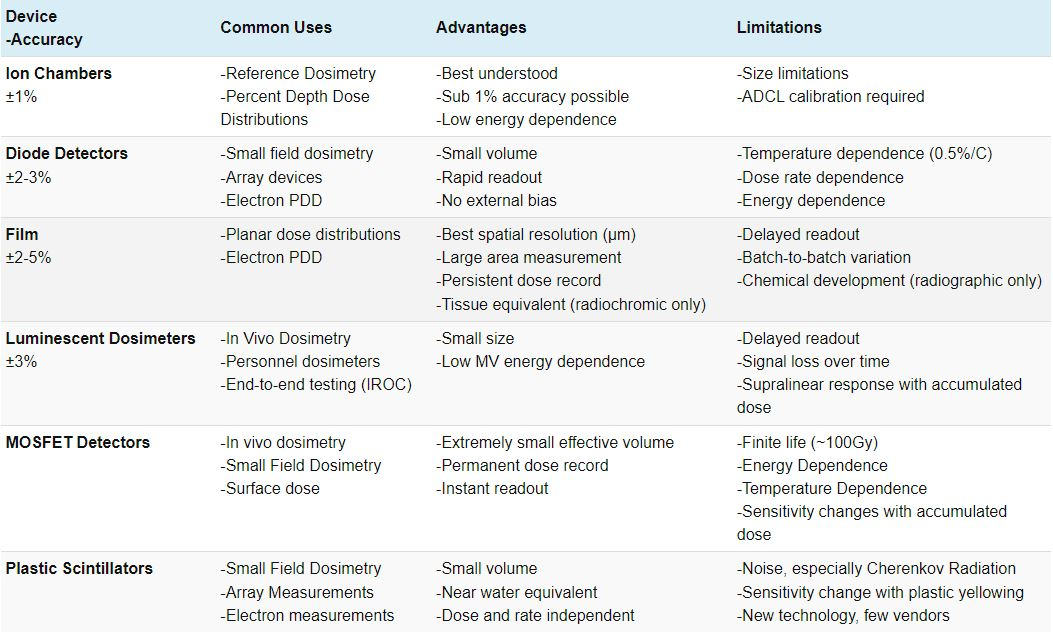
\includegraphics[width=0.8\textwidth]{Imagens/comparacaoDetectores.JPG}
		}%
		\caption{Comparação entre Detectores.}
		\label{fig:comparacaoDetectores}
	\end{figure}



\section{Dosímetros Padrão Primário}

\subsection*{Calorímetros}

		O calorímetro utilizado para a dosimetria das radiações é um dispositivo projetado para medir a \textcolor{MediumOrchid}{\textit{\textbf{quantidade de energia térmica liberada quando a radiação ionizante interage com um material sensível}}}. O princípio básico de funcionamento de um calorímetro é a \textcolor{MediumOrchid}{\textit{\textbf{conversão da energia depositada pela radiação em calor e a medição desse calor gerado}}}, uma vez que a variação da temperatura na água devido a 1 Gy de dose absorvida é:
		
			\begin{equation}
				1 \; Gy = 2.4 \times 10^{-4}\;{}^{\circ}C \; na \; agua
			\end{equation}

		A determinação da dose absorvida através de um calorímetro se dá da seguinte forma:

		\begin{enumerate}
			\item \textcolor{DarkTurquoise}{\textbf{Material sensível:}} O calorímetro é construído com um material sensível à radiação que tem a capacidade de converter a energia depositada pela radiação em calor de forma eficiente. Esse material pode ser um cristal, um líquido ou um polímero termossensível.
			\item \textcolor{DarkTurquoise}{\textbf{Calorimetria adiabática:}} O calorímetro é projetado para ser termicamente isolado do ambiente externo, de forma que não haja troca significativa de calor com o ambiente durante a medida. Isso é chamado de calorimetria adiabática.
			\item \textcolor{DarkTurquoise}{\textbf{Absorção de energia:}} Quando a radiação ionizante interage com o material sensível, ela deposita energia nesse material causando excitações ou ionizações que eventualmente levam os elétrons a se moverem para camadas mais altas, o que faz com que as moléculas vibrem mais rapidamente, que é basicamente o conceito por trás do calor. De fato, toda a radiação absorvida eventualmente aparece como calor e, portanto, isso pode ser medido com uma precisão muito alta em teoria.
			\item \textcolor{DarkTurquoise}{\textbf{Medida da temperatura:}} A temperatura do calorímetro é medida utilizando sensores de temperatura sensíveis e precisos. Esses sensores podem ser termopares, termorresistências (RTDs) ou termistores.
			\item \textcolor{DarkTurquoise}{\textbf{Calibração:}} O calorímetro deve ser calibrado previamente usando fontes de radiação de referência para estabelecer uma relação entre a quantidade de calor gerado e a dose de radiação absorvida.
			\item \textcolor{DarkTurquoise}{\textbf{Cálculo da dose:}} Com base na medição da temperatura e nas características do calorímetro, é possível calcular a dose de radiação absorvida pelo material sensível, com base nos parâmetros prévios de calibração. 
		\end{enumerate}

		Os calorímetros utilizados na dosimetria de radiação fornecem uma medida direta da quantidade de energia depositada pela radiação na água, permitindo uma determinação precisa da dose absorvida. No entanto, eles requerem uma calibração cuidadosa e podem ser mais complexos em comparação com outros métodos de dosimetria de radiação, como os TLDs ou os OSLDs, pois a variação de temperatura é muito pequena, necessitando de um equipamento com uma precisão muito alta, e, portanto, não é considerado muito prático.


\subsection*{Dosímetro de Fricke}

		O dosímetro de Fricke é um tipo de dosímetro químico utilizado para medir a dose absorvida de radiação . Ele é baseado na propriedade do sal de Fricke, uma solução de sulfato ferroso  em ácido sulfúrico (\ce{H2SO4}), de sofrer uma mudança de cor devido aos íons férricos (concentração) formados quando exposto à radiação ionizante.

		O processo de funcionamento do dosímetro de Fricke se dá pela seguinte maneira:

		\begin{enumerate}
			\item \textcolor{DarkTurquoise}{\textbf{Preparação do dosímetro:}} Uma solução de sal de Fricke é preparada cuidadosamente em laboratório, utilizando sulfato ferroso, cloreto de sódio, ácido sulfúrico e água. A concentração da solução é ajustada para fornecer uma resposta linear à radiação dentro da faixa de dose de radiação avaliada. Normalmente é utilizado uma concentração de 1 mmol/L de sulfato ferroso, 1 mmol/L de \ce{NaCl} e 0.4 mol/L de \ce{H2SO4}.
			\item \textcolor{DarkTurquoise}{\textbf{Exposição à radiação:}} O dosímetro de Fricke é exposto à radiação ionizante que se deseja medir a dose absorvida. A radiação interage com os íons da solução de Fricke, causando uma série de reações químicas;
			\item \textcolor{DarkTurquoise}{\textbf{Formação de íons férricos:}} A radiação ionizante converte os íons ferrosos (\ce{Fe^2+}) em íons férricos (\ce{Fe^3+}). Essa conversão ocorre devido à oxidação do ferro induzida pelo processo de ionização.
			\item \textcolor{DarkTurquoise}{\textbf{Mudança de cor:}} Os íons férricos (\ce{Fe^3+}) formados na solução de Fricke têm uma coloração diferente dos íons ferrosos (\ce{Fe^2+}). A mudança de cor é geralmente uma mudança do tom verde para o tom azul.
			\item \textcolor{DarkTurquoise}{\textbf{Medição da absorção de radiação:}} A magnitude da mudança de cor (concentração de íons férricos) é proporcional à quantidade de radiação absorvida pela solução de Fricke. Essa concentração de íons férricos pode ser quantificada por meio de técnicas espectrofotométricas, que medem a absorção de luz em uma determinada faixa de comprimento de onda. (Picos de absorção UV em 224 nm e 304 nm).
			\item \textcolor{DarkTurquoise}{\textbf{Cálculo da dose de radiação absorvida:}} A magnitude da mudança de cor é relacionada a uma dose de radiação específica por meio de uma curva de calibração pré-determinada. Com base nessa curva, é possível determinar a dose de radiação absorvida pelo dosímetro de Fricke.
		\end{enumerate}

		Infelizmente, nem todas as energias dos fótons criam o mesmo número de reações, então existem tabelas de “valores G” que são o número de moléculas produzidas por 100 eV de energia absorvida. O número é de cerca de 15,5 moléculas por 100 eV absorvidos e esse valor de G não muda muito para energias usadas em radiação oncológica.

		O dosímetro de Fricke é um método amplamente utilizado em pesquisas em radioterapia, permitindo uma medição precisa da dose de radiação absorvida. No entanto, requer preparação cuidadosa da solução de Fricke, calibração adequada e análise precisa da concentração de íons férricos para obter resultados confiáveis.

\section{Quantidades Operacionais}

	A Comissão Internacional de Unidades e Medidas de Radiação (ICRU) é responsável por fornecer recomendações sobre as grandezas dosimétricas e unidades utilizadas na dosimetria de proteção radiológica. Essas recomendações estabelecem diretrizes e padrões internacionais para a medição e expressão das grandezas relacionadas à radiação ionizante. A aplicação prática dessas grandezas e unidades na proteção radiológica é estabelecida pela Comissão Internacional de Proteção Radiológica (ICRP), que é responsável por desenvolver orientações e regulamentações para garantir a segurança dos trabalhadores e do público em relação à radiação ionizante.

	As grandezas operacionais são grandezas dosimétricas específicas que são definidas para permitir medições práticas tanto no monitoramento de área quanto no monitoramento individual de radiação. Elas são projetadas para facilitar a avaliação da exposição à radiação ionizante e garantir a conformidade com os limites estabelecidos para a proteção radiológica.

	Na proteção radiológica, a radiação é classificada como de baixa penetração ou alta penetração com base em qual dose equivalente está mais próxima de seu valor limite. Essa classificação é relevante para determinar as medidas de proteção necessárias. Tipicamente, a radiação de \textcolor{MediumOrchid}{\textit{\textbf{"baixa penetração"}}} se refere a fótons abaixo de \textcolor{MediumOrchid}{\textit{\textbf{15 keV (baixa energia)}}} e radiação \textcolor{MediumOrchid}{\textit{\textbf{beta}}} (partículas carregadas emitidas por fontes radioativas). Essa classificação ajuda a direcionar o tipo de monitoramento e proteção adequados para diferentes tipos de radiação.

	No monitoramento de área, duas grandezas são definidas para estabelecer a relação entre o campo de radiação externa e o equivalente de dose efetiva no fantoma esférico da ICRU em uma profundidade específica $(d)$ e em uma direção especificada $(\Omega)$. Essas grandezas são utilizadas para quantificar a exposição à radiação em uma determinada área e direção específicas.

	\begin{enumerate}
		\item O \textcolor{DarkTurquoise}{\textbf{Equivalente de dose ambiente}} ($H^{\ast}(d)$) é uma grandeza utilizada para \textcolor{MediumOrchid}{\textit{\textbf{quantificar a dose de radiação em um ambiente com radiação de alta penetração}}}. Essa grandeza é avaliada em uma profundidade específica, sendo $d = 10 \text{ mm}$ a profundidade escolhida. O equivalente de dose ambiente para radiação de alta penetração é denotado como $H^{\ast}(10)$.
		\item O \textcolor{DarkTurquoise}{\textbf{Equivalente de dose direcional}} ($H^{\prime}(d, \Omega)$) é outra grandeza utilizada no monitoramento de área e é aplicável tanto para \textcolor{MediumOrchid}{\textit{\textbf{radiação de alta penetração quanto para radiação de baixa penetração}}}. A profundidade escolhida depende do tipo de radiação em questão:
		\begin{itemize}
			\item Para radiação de \textcolor{DarkTurquoise}{\textbf{alta penetração}}, a profundidade escolhida é \textcolor{MediumOrchid}{\textit{\textbf{$d = 10\; mm$}}}, e o equivalente de dose direcional é denotado como \textcolor{MediumOrchid}{\textit{\textbf{$H^{\prime}(10, \Omega)$}}}.
			\item Para radiação de \textcolor{DarkTurquoise}{\textbf{baixa penetração}}, as profundidades relevantes são \textcolor{MediumOrchid}{\textit{\textbf{$d = 0.07 \;mm$}}} na pele e \textcolor{MediumOrchid}{\textit{\textbf{$d = 3\; mm$}}} no cristalino do olho. As grandezas são denotadas como \textcolor{MediumOrchid}{\textit{\textbf{$H^{\ast}(0.07)$}}} e \textcolor{MediumOrchid}{\textit{\textbf{$H^{\prime}(0.07, \Omega)$}}} para a pele, e \textcolor{MediumOrchid}{\textit{\textbf{$H^{\ast}(3)$}}} e \textcolor{MediumOrchid}{\textit{\textbf{$H^{\prime}(3, \Omega)$}}} para o cristalino do olho.
		\end{itemize}
	\end{enumerate}

	No monitoramento individual, o \textcolor{MediumOrchid}{\textit{\textbf{equivalente de dose pessoal ($H_{\text{p}}(d)$)}}} é uma grandeza que representa o equivalente de dose em tecido mole abaixo de um ponto específico no corpo, em uma profundidade (d) específica. Essa definição é estabelecida no Capítulo 16 das recomendações e diretrizes da Comissão Internacional de Unidades e Medidas de Radiação (ICRU). O equivalente de dose pessoal é utilizado para avaliar a \textcolor{MediumOrchid}{\textit{\textbf{exposição individual à radiação ionizante}}} e é uma medida importante para a proteção radiológica.

	\begin{enumerate}
		\item No caso de \textcolor{DarkTurquoise}{radiação de \textbf{alta penetração}}, uma profundidade específica de \textcolor{MediumOrchid}{\textit{\textbf{$d = 10\; mm$}}} é escolhida para a avaliação do equivalente de dose pessoal. Essa grandeza é denotada como \textcolor{MediumOrchid}{\textit{\textbf{$H_{\text{p}}(10)$}}} e representa o equivalente de dose em tecido mole a uma profundidade de 10 mm.
		\item Para a \textcolor{DarkTurquoise}{radiação de \textbf{baixa penetração}}, são relevantes duas profundidades específicas:
		\begin{itemize}
			\item \textcolor{DarkTurquoise}{\textbf{$H_{\text{p}}(0.07)$}}: Este é o equivalente de dose pessoal na pele a uma profundidade de \textcolor{MediumOrchid}{\textit{\textbf{$d = 0.07 \; mm$}}}.
			\item \textcolor{DarkTurquoise}{\textbf{$H_{\text{p}}(3)$}}: Este é o equivalente de dose pessoal no cristalino do olho a uma profundidade de \textcolor{MediumOrchid}{\textit{\textbf{$d = 3\; mm$}}}.
		\end{itemize}
	\end{enumerate}

	O \textcolor{MediumOrchid}{\textit{\textbf{equivalente de dose pessoal ($H_{\text{p}}(d)$)}}} pode ser medido utilizando um dosímetro que é colocado na \textcolor{MediumOrchid}{\textit{\textbf{superfície do corpo}}} e coberto com um material que tem propriedades equivalentes ao tecido apropriado. O dosímetro é projetado para registrar a dose de radiação em uma profundidade específica do tecido mole, permitindo a quantificação do equivalente de dose pessoal em diferentes partes do corpo.

\section{Monitores de Área}

	Os detectores de área são instrumentos de radiação utilizados como \textcolor{MediumOrchid}{\textit{\textbf{monitores de levantamento}}} para medir a radiação em uma \textcolor{MediumOrchid}{\textit{\textbf{área}}} específica. Esses detectores podem ser categorizados em dois tipos principais: \textcolor{MediumOrchid}{\textit{\textbf{detectores preenchidos com gás}}} e \textcolor{MediumOrchid}{\textit{\textbf{detectores de estado sólido}}}, como detectores cintiladores ou semicondutores.

	Os detectores preenchidos com gás têm uma forma cilíndrica e consistem em uma parede externa e um eletrodo central, que são isolados um do outro. O material da parede do detector varia dependendo do tipo de detector. Por exemplo, os detectores de câmara de ionização usam materiais equivalentes a tecidos, enquanto outros tipos de detectores podem empregar latão ou cobre.

	A operação de um detector preenchido com gás é determinada pelo seu \textcolor{MediumOrchid}{\textit{\textbf{design}}} e pela \textcolor{MediumOrchid}{\textit{\textbf{tensão aplicada entre os eletrodos}}} (\ref{fig:regiaoDetecGas}). Essa operação resulta em uma das três regiões operacionais principais: a região de ionização (Região B), a região proporcional (Região C) ou a região Geiger-Müller (GM) (Região E). Nas regiões de recombinação e proporcionalidade limitada (Regiões A e D, respectivamente), conforme mostrado na \ref{fig:regiaoDetecGas}, não são utilizadas em medidores de levantamento.

	\begin{figure}[h]
		\centering
		\fcolorbox{DarkTurquoise}{white}{%
			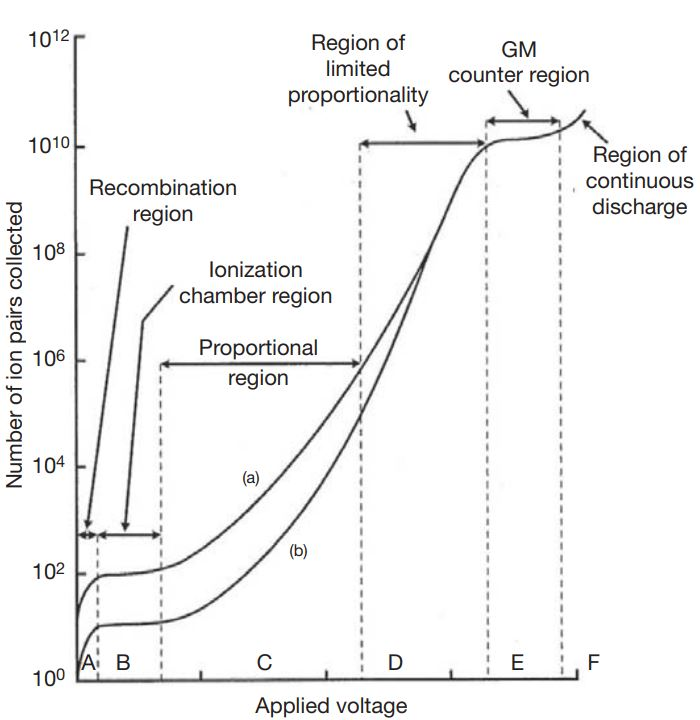
\includegraphics[width=0.5\textwidth]{Imagens/regiaoDetecGas.JPG}
		}%
		\caption{Detectores preenchidos com gás exibem várias regiões de operação, cada uma associada a diferentes características e aplicações. Essas regiões são representadas da seguinte forma: Região A: Região de recombinação; Região B: Região de saturação iônica; Região C: Região de proporcionalidade; Região D: Região de proporcionalidade limitada; Região E: Região Geiger-Müller (GM) No gráfico "sinal versus tensão aplicada", essas regiões representam o comportamento do detector para diferentes energias de partículas. A curva (a) corresponde a partículas beta de 1 MeV, enquanto a curva (b) representa partículas beta de 100 keV.}
		\label{fig:regiaoDetecGas}
	\end{figure}

	Os detectores preenchidos com gás são amplamente utilizados devido à sua capacidade de detectar uma \textcolor{MediumOrchid}{\textit{\textbf{ampla faixa de energia e tipos de radiação}}}. Eles são especialmente úteis para medições de dose ambiente e monitoramento da exposição à radiação em locais de trabalho. A resposta dos detectores preenchidos com gás é geralmente linear e proporcional à energia e taxa de dose da radiação incidente.

	Por outro lado, os \textcolor{MediumOrchid}{\textit{\textbf{detectores de estado sólido}}}, como detectores cintiladores ou semicondutores, são construídos a partir de materiais sólidos que são sensíveis à radiação. Esses detectores utilizam propriedades como \textcolor{MediumOrchid}{\textit{\textbf{cintilação}}} (emissão de luz quando excitados por radiação) ou alteração nas características elétricas do material para medir a radiação. Os detectores de estado sólido têm várias vantagens, incluindo \textcolor{MediumOrchid}{\textit{\textbf{alta sensibilidade}}}, \textcolor{MediumOrchid}{\textit{\textbf{resposta rápida}}} e \textcolor{MediumOrchid}{\textit{\textbf{tamanho compacto}}}. Eles são comumente usados em aplicações de monitoramento de radiação em tempo real, como em radioterapia ou controle de qualidade em radiografia industrial.


	\begin{exemplo}[Características dos Monitores de Área a gás]
		\begin{itemize}
			\item \textcolor{DarkTurquoise}{\textbf{Os detectores de área estão disponíveis em várias formas e tamanhos, projetados para atender a aplicações específicas}}. Eles podem ser portáteis ou fixos, dependendo das necessidades de medição (\ref{fig:monitoresDeAreaGaS}).
			\item \textcolor{DarkTurquoise}{\textbf{Para evitar a formação de íons negativos, o que aumentaria o tempo de coleta de carga e limitaria a capacidade de taxa de dose do monitor, geralmente são utilizados gases não eletronegativos nos detectores preenchidos com gás}}. Isso ocorre porque os íons têm mobilidade significativamente mais lenta em comparação com os elétrons. Os gases nobres, como o hélio e o argônio, são comumente empregados nesses detectores.
			\item \textcolor{DarkTurquoise}{\textbf{Detectores de área destinados à medição de radiação beta e gama apresentam uma janela fina na extremidade para detectar radiação de baixa penetração}}. A eficiência gama desses detectores é relativamente baixa, geralmente alguns por cento, devido à absorção pelas paredes do detector. No entanto, a resposta para partículas beta que entram no detector é próxima de 100\%.
			\item \textcolor{DarkTurquoise}{\textbf{Monitores de radiação gama baseados no princípio Geiger-Müller (GM) são conhecidos por sua alta sensibilidade}}. Esses detectores geralmente possuem tamanhos de tubo menores em comparação com detectores do tipo câmara de ionização. Eles são capazes de detectar radiação gama de forma eficiente e são amplamente utilizados para monitoramento de radiação em várias aplicações. 
			\item  \textcolor{DarkTurquoise}{\textbf{Os detectores podem operar no modo "pulso" ou no modo "nível médio" ou modo de corrente, dependendo da eletrônica utilizada}}. Contadores proporcionais e Geiger-Müller são tipicamente operados no modo de pulso.
			\item \textcolor{DarkTurquoise}{\textbf{Devido ao tempo de resposta finito, que se refere ao tempo necessário para que o detector retorne ao seu estado normal após registrar um pulso, esses detectores podem atingir a saturação em campos de radiação de alta intensidade}}. Para medições de taxa de dose mais alta, câmaras de ionização operando no modo de corrente são mais adequadas.
		\end{itemize}
	\end{exemplo}

	\begin{figure}[h]
		\centering
		\fcolorbox{DarkTurquoise}{white}{%
			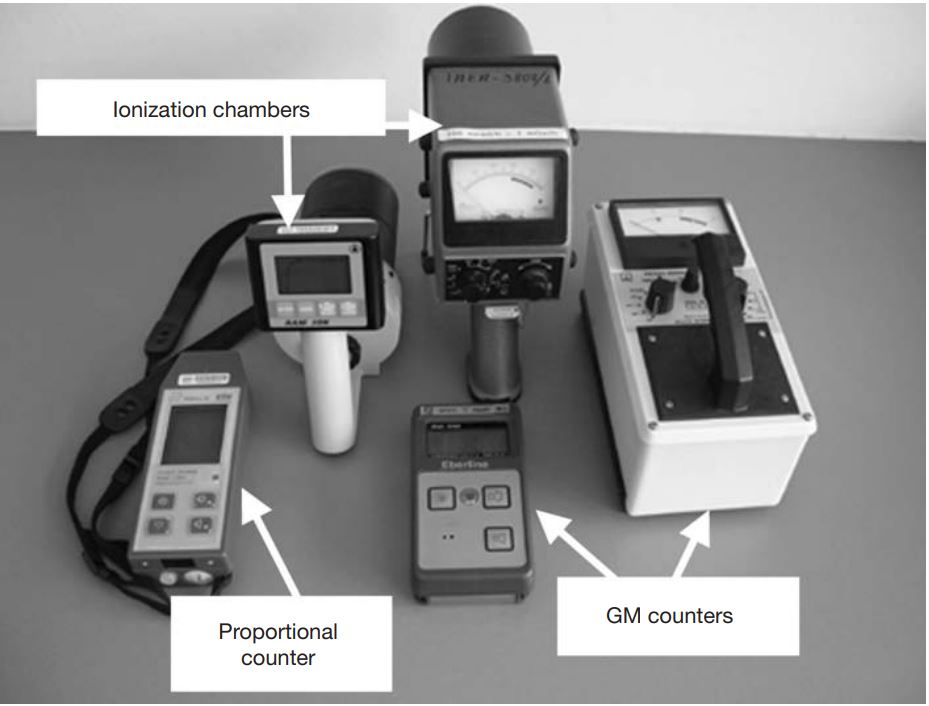
\includegraphics[width=0.5\textwidth]{Imagens/monitoresDeAreaGaS.JPG}
		}%
		\caption{Monitores de levantamento de área comumente usados para medições de nível de proteção contra radiação: câmaras de ionização, contador proporcional e contador GM.}
		\label{fig:monitoresDeAreaGaS}
	\end{figure}
	
\subsubsection*{Câmaras de Ionização}

	Na região de ionização de uma câmara de ionização, \textcolor{MediumOrchid}{\textit{\textbf{o número de íons primários (positivos ou negativos) coletados é diretamente proporcional à energia depositada pelas trajetórias das partículas carregadas dentro do volume do detector}}}. Esses íons primários são produzidos quando a radiação ionizante interage com o material sensível da câmara de ionização.

	As câmaras de ionização são \textcolor{MediumOrchid}{\textit{\textbf{capazes de discriminar diferentes tipos de partículas}}} com base em suas características de transferência linear de energia (LET). Partículas com diferentes LETs depositam diferentes quantidades de energia ao interagirem com o material da câmara de ionização, o que permite distinguir e medir diferentes tipos de partículas (conforme mostrado na \ref{fig:regiaoDetecGas}).

	Ao medir radiação de\textcolor{MediumOrchid}{\textit{\textbf{ fótons de alta energia}}}, como raios X ou raios gama, o uso de \textcolor{MediumOrchid}{\textit{\textbf{capas de compensação}}} é necessário. Essas capas de compensação são materiais com \textcolor{MediumOrchid}{\textit{\textbf{características de atenuação semelhantes aos tecidos humanos}}} e são usadas para simular a interação da radiação com o corpo humano. Elas ajudam a \textcolor{MediumOrchid}{\textit{\textbf{aumentar a eficiência de detecção}}} e garantem que a resposta da câmara de ionização seja representativa da dose absorvida no tecido humano.

	Ao medir radiação de \textcolor{MediumOrchid}{\textit{\textbf{fótons de alta energia}}}, como raios X ou raios gama, o uso de \textcolor{MediumOrchid}{\textit{\textbf{capas de buildup}}} é necessário. Essas capas de buildup ajudam a aumentar a eficiência de detecção ao medir fótons de alta energia. No entanto,\textcolor{MediumOrchid}{\textit{\textbf{as capas de buildup devem ser removidas ao medir fótons de energia mais baixa (10-100 keV) e partículas beta}}}. Isso ocorre porque a presença das capas de buildup pode causar atenuação excessiva da radiação de baixa energia ou resultar em uma resposta distorcida para partículas beta.

\subsubsection*{Contadores Proporcionais}

	Na região proporcional, \textcolor{MediumOrchid}{\textit{\textbf{os íons primários gerados pela interação da radiação com o material do detector são amplificados por meio do processo de multiplicação de carga}}}. Esse processo ocorre por meio de \textcolor{MediumOrchid}{\textit{\textbf{colisões}}} entre os \textcolor{MediumOrchid}{\textit{\textbf{íons primários}}} e as \textcolor{MediumOrchid}{\textit{\textbf{moléculas de gás}}} presentes no detector. A energia ganha pelos íons primários durante as colisões sucessivas pode ser suficiente para causar ionização adicional dentro do detector, resultando em uma \textcolor{MediumOrchid}{\textit{\textbf{amplificação do sinal}}}.

	A amplificação nos contadores proporcionais é geralmente alcançada por meio de um \textcolor{MediumOrchid}{\textit{\textbf{eletrodo central}}} fino entre o eletrodo externo e o cátodo. O campo \textcolor{MediumOrchid}{\textit{\textbf{elétrico intenso}}} próximo ao eletrodo central facilita a ionização por colisão, permitindo que os íons primários causem uma ionização adicional antes de serem coletados. A amplificação nos contadores proporcionais resulta em um \textcolor{MediumOrchid}{\textit{\textbf{fator de multiplicação}}} da ordem de \textcolor{MediumOrchid}{\textit{\textbf{$10^3$ a $10^4$}}}. Isso significa que cada partícula incidente gera um sinal amplificado que é várias vezes maior do que o sinal original de íons primários.

	Os contadores proporcionais oferecem \textcolor{MediumOrchid}{\textit{\textbf{maior sensibilidade em comparação com as câmaras de ionização devido à amplificação do sinal}}}. Eles são adequados para medições em \textcolor{MediumOrchid}{\textit{\textbf{campos de radiação de baixa intensidade}}}, onde a detecção precisa de partículas individuais é necessária. A \textcolor{MediumOrchid}{\textit{\textbf{quantidade de carga coletada a partir de cada interação dentro do contador proporcional é diretamente proporcional à quantidade de energia depositada no gás}}} pela interação. Isso permite que a dose absorvida seja estimada com base na carga coletada.

\subsubsection*{Monitores de área para nêutrons}

	Os medidores de área para nêutrons são projetados para operar na \textcolor{MediumOrchid}{\textit{\textbf{região proporcional}}}, o que permite discriminar facilmente a radiação de fundo de fótons.

	\begin{exemplo}[Características dos Monitores de De Nêutrons:]
		\begin{itemize}
			\item \textcolor{DarkTurquoise}{\textbf{Detectores de nêutrons térmicos}} são comumente revestidos com um composto de boro na parede interna ou preenchidos com gás \ce{BF3}. 
			
			\item \textcolor{DarkTurquoise}{\textbf{O boro é eficaz na detecção de nêutrons térmicos}}, pois quando um nêutron térmico interage com um núcleo de \ce{^{10}B}, ocorre uma reação (n, alfa), e as partículas alfa resultantes podem ser facilmente detectadas por meio de suas interações de ionização.

			\item Para detectar \textcolor{DarkTurquoise}{\textbf{nêutrons rápidos}}, o mesmo detector é envolvido por um moderador composto por um material rico em hidrogênio (\ref{fig:monitorNeutron}). Essa configuração transforma o conjunto em um contador de nêutrons rápidos. Os nêutrons rápidos que interagem com o moderador são termalizados (perdem energia) e subsequentemente detectados por um contador de \ce{BF3} localizado dentro do moderador.
			
			\item \textcolor{DarkTurquoise}{\textbf{Filtros de compensação}} são empregados para reduzir a resposta excessiva à faixa térmica, garantindo que a resposta do detector siga os fatores de ponderação de radiação da ICRP ($w_{\text{R}}$). Dessa forma, a saída do detector é aproximadamente proporcional ao equivalente de dose em tecido mole em uma ampla faixa de espectros de energia de nêutrons.
			
			\item Outros detectores de nêutrons, como aqueles baseados em \ce{^3He} (hélio-3), também operam com os mesmos princípios. 
		\end{itemize}
	\end{exemplo}

	\begin{figure}[h]
		\centering
		\fcolorbox{DarkTurquoise}{white}{%
			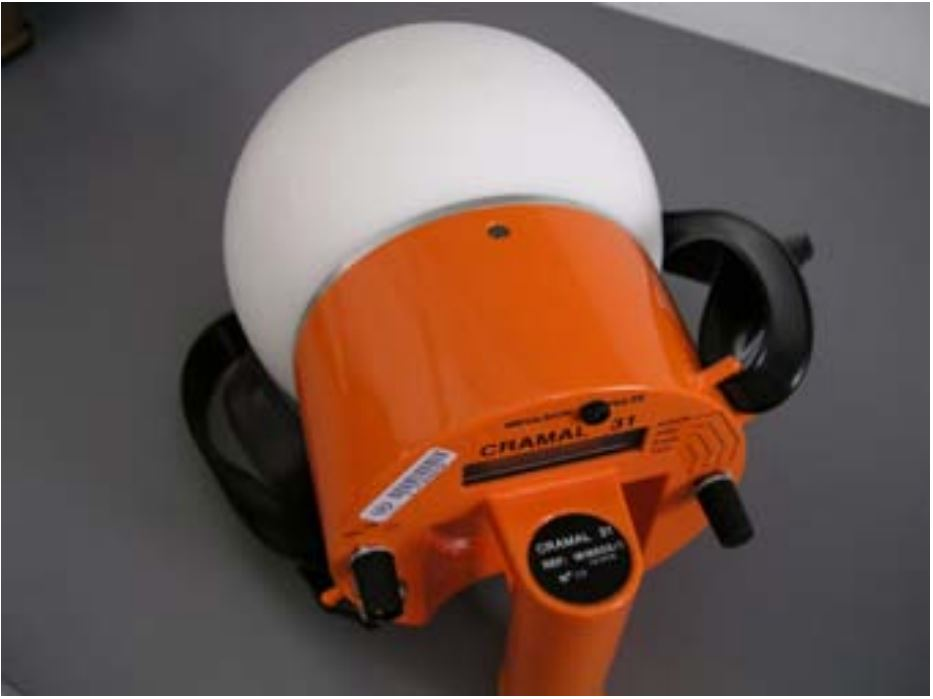
\includegraphics[width=0.5\textwidth]{Imagens/monitorNeutron.JPG}
		}%
		\caption{Medidor de taxa equivalente de dose de nêutrons com uma esfera de polietileno termalizante com diâmetro de 20 cm.}
		\label{fig:monitorNeutron}
	\end{figure}

\subsubsection*{Contadores Geiger-Müller}

	Na região de operação GM, ocorre uma \textcolor{MediumOrchid}{\textit{\textbf{descarga que se espalha por todo o volume do detector}}}, e a \textcolor{MediumOrchid}{\textit{\textbf{altura do pulso}}} se torna \textcolor{MediumOrchid}{\textit{\textbf{independente}}} da ionização primária ou da energia das partículas interagentes. Isso ocorre devido à \textcolor{MediumOrchid}{\textit{\textbf{multiplicação do gás}}} ao longo de todo o comprimento do ânodo dentro do contador GM. 

	Portanto, os contadores GM são conhecidos por sua considerável \textcolor{MediumOrchid}{\textit{\textbf{amplificação de carga}}}, que pode ser de nove a dez ordens de magnitude. Essa alta amplificação de carga permite a \textcolor{MediumOrchid}{\textit{\textbf{detecção de níveis muito baixos de radiação}}}, tornando-os adequados para aplicações em que é necessário detectar e monitorar a \textcolor{MediumOrchid}{\textit{\textbf{presença de radiação}}} em áreas de ocupação pública, como salas de tratamento de radioterapia, testes de vazamento e detecção de contaminação radioativa.

	É importante ressaltar que os detectores GM \textcolor{MediumOrchid}{\textit{\textbf{não podem ser operados além da região GM}}}, uma vez que ocorre \textcolor{MediumOrchid}{\textit{\textbf{descarga contínua}}}. Portanto, eles são utilizados principalmente como indicadores qualitativos da presença de radiação e não são adequados para medições precisas de dose. Além disso, os contadores GM apresentam uma \textcolor{MediumOrchid}{\textit{\textbf{alta dependência energética em baixas energias de fótons}}} e não são adequados para uso em campos de \textcolor{MediumOrchid}{\textit{\textbf{radiação pulsada}}}. Sua resposta também pode ser afetada por \textcolor{MediumOrchid}{\textit{\textbf{variações de temperatura}}}.

	Os detectores GM têm \textcolor{MediumOrchid}{\textit{\textbf{tempos mortos longos}}}, tipicamente variando de dezenas a centenas de milissegundos. Isso significa que eles \textcolor{MediumOrchid}{\textit{\textbf{não são adequados para medições precisas em altas taxas de contagem}}}, pois podem ficar temporariamente inativos e mostrar leituras zeradas. Nesses casos, as câmaras de ionização são mais apropriadas para medições em áreas com altas taxas de radiação.

\subsubsection*{Detectores de Cintilação}

	Os detectores de cintilação são dispositivos que utilizam o fenômeno da cintilação, que é a emissão de luz após a absorção de radiação, para detectar e quantificar a radiação incidente. Os detectores de cintilação pertencem à classe de detectores de estado sólido, e certos cristais orgânicos e inorgânicos são capazes de emitir cintilação quando excitados por radiação. Esses materiais são conhecidos como fósforos.

	Existem diferentes tipos de fósforos cintiladores utilizados em detectores de cintilação. Os fósforos com números atômicos elevados, como o tálio, são comumente usados para detectar raios gama, enquanto os cintiladores de plástico são frequentemente empregados para detectar partículas beta.  Os fósforos cintiladores podem ser compostos por substâncias orgânicas sólidas, como o antraceno e o estilbeno, ou por materiais inorgânicos ativados com tálio, como o \ce{NaI}(\ce{Tl}) ou o \ce{CsI}(\ce{Tl}). Esses materiais têm a capacidade de absorver a energia da radiação e emitir cintilação proporcional à quantidade de energia absorvida.

	Para converter o pulso de luz emitido pelo fósforo cintilador em um pulso elétrico mensurável, um tubo fotomultiplicador (PMT) é acoplado de forma óptica ao fósforo. O PMT amplifica o sinal luminoso e o converte em um sinal elétrico proporcional. Em alguns medidores de área, fotodiodos podem ser usados como uma alternativa aos PMTs para a detecção da cintilação.

	Os detectores de cintilação oferecem alta eficiência de detecção e uma ampla faixa dinâmica, permitindo a detecção de baixos níveis de radiação, bem como altas taxas de contagem. Eles são amplamente utilizados em diversas aplicações, como monitoramento de radiação em ambientes de trabalho, pesquisa em física nuclear, medicina nuclear e detecção de radiação em geral.

\subsubsection*{Detectores Semicondutores}

	Os detectores de semicondutores são dispositivos amplamente utilizados para a detecção e medição de radiação ionizante. Existem dois tipos principais de detectores de semicondutores: detectores de condutividade em volume e detectores de junção.

	\

	\textcolor{MediumOrchid}{\Large\LobsterTwo\textbf{Detectores de Condutividade em Volume}}
	\begin{itemize}
		\item Os \textcolor{DarkTurquoise}{\textbf{detectores de condutividade em volume}} são feitos de semicondutores \textcolor{DarkTurquoise}{\textbf{intrínsecos}} com \textcolor{DarkTurquoise}{\textbf{alta resistividade volumétrica}}, como o sulfeto de cádmio (\ce{CdS}) ou o seleneto de cádmio (\ce{CdSe}).
		\item Quando expostos à radiação, esses detectores funcionam de maneira semelhante às câmaras de ionização de estado sólido. Eles dependem da medição de mudanças na condutividade elétrica dentro do material semicondutor.
		\item A radiação ionizante cria pares de elétrons e lacunas no semicondutor, alterando a condutividade elétrica do material. Essas mudanças na condutividade são detectadas e quantificadas para determinar a quantidade de radiação incidente.
		\item Os detectores de condutividade em volume oferecem \textcolor{DarkTurquoise}{\textbf{alta eficiência de detecção}}, \textcolor{DarkTurquoise}{\textbf{excelente resolução energética}} e \textcolor{DarkTurquoise}{\textbf{resposta rápida}}. Eles são frequentemente usados em aplicações que exigem alta sensibilidade, como espectroscopia de raio-X e detecção de partículas.
	\end{itemize}

	\textcolor{MediumOrchid}{\Large\LobsterTwo\textbf{Detectores de Junção}}
	\begin{itemize}
		\item Os detectores de junção são formados por semicondutores \textcolor{DarkTurquoise}{\textbf{extrínsecos}}, como o \textcolor{DarkTurquoise}{\textbf{silício}} ou o \textcolor{DarkTurquoise}{\textbf{germânio,}} dopados com pequenas quantidades de impurezas.
		\item Aplicando um \textcolor{DarkTurquoise}{\textbf{bias reverso}} aos detectores, eles também funcionam como \textcolor{DarkTurquoise}{\textbf{câmaras de ionização de estado sólido}} quando expostos à radiação ionizante.
		\item A radiação ionizante cria pares de elétrons e lacunas na região de junção do semicondutor, alterando a corrente elétrica que flui através da junção.
		\item Essas alterações na corrente são medidas e quantificadas para determinar a quantidade de radiação incidente.
		\item Os detectores de junção oferecem \textcolor{DarkTurquoise}{\textbf{alta resolução energética}}, \textcolor{DarkTurquoise}{\textbf{excelente linearidade}} e \textcolor{DarkTurquoise}{\textbf{resposta rápida}}. Eles são comumente usados em espectrometria de raios-X, espectrometria gama e detecção de partículas.
	\end{itemize}

	Tanto os detectores de condutividade em volume quanto os detectores de junção têm a vantagem de serem construídos em estado sólido, o que os torna compactos, duráveis e adequados para uma variedade de aplicações.

\subsection*{Propriedade dos Monitores de Área}

\subsubsection*{Sensibilidade}

	A sensibilidade (S) de um detector de radiação é definida como o inverso do coeficiente de calibração (N). Uma sensibilidade mais alta indica uma maior resposta à radiação.

	Medidores de área baseados em câmaras de ionização podem cobrir uma ampla faixa de taxas de dose equivalente através do uso de resistências, volumes maiores do detector ou gases do detector em pressões mais altas. Esses fatores permitem uma ampla gama de medidas, normalmente variando de 1 mSv/h a 1 Sv/h.

	Sistemas baseados em Geiger-Müller (GM), devido ao seu tempo de resposta finito, podem saturar além de algumas milhares de contagens por segundo. No entanto, contadores com baixo tempo morto ou circuitos de correção de tempo morto permitem que os detectores GM operem em campos de radiação de alta intensidade.

	Sistemas baseados em cintilação geralmente são mais sensíveis do que os contadores GM devido à sua maior eficiência de conversão de raios gama e amplificação por dínodos. Eles são comumente utilizados para medições em níveis muito baixos de radiação, como monitoramento de contaminação e pesquisas de detecção de fontes perdidas. No entanto, também podem ser utilizados em níveis mais altos de radiação devido ao seu tempo de resposta relativamente curto, geralmente na faixa de alguns microssegundos ou menos, em comparação com os contadores GM.

\subsubsection*{Dependência Energética}

	Os medidores de área são dispositivos utilizados para medir a exposição à radiação em uma determinada área. Eles são calibrados em relação a qualidades específicas do feixe de radiação, o que significa que sua resposta é otimizada para uma faixa de energia conhecida. No entanto, na prática clínica, os medidores de área são frequentemente utilizados em situações onde o campo de radiação é complexo ou desconhecido. Portanto, é essencial que esses medidores tenham uma baixa dependência de energia, o que significa que sua resposta não deve variar significativamente em uma ampla faixa de energias.

	No passado, os medidores de área eram projetados de forma a ter uma resposta de energia plana, ou seja, sua sensibilidade era mantida constante em diferentes energias de radiação. Isso era feito para que a resposta do medidor pudesse ser diretamente relacionada à grandeza de exposição ou kerma no ar, que são medidas importantes na dosimetria da radiação.

	Quando estamos interessados em medir a dose equivalente, que é uma grandeza que leva em consideração o tipo de radiação e seu efeito biológico, a resposta de um medidor de área em relação à energia deve variar de acordo a euqação:
	
	\begin{equation}
		N_{\text{H}^{\ast}} = \frac{H^{\ast}(10)}{M} = \frac{\left[H^{\ast}(10)/(K_{\text{ar}})_{\text{ar}}
		\right]}{\left[(K_{\text{ar}})_{\text{ar}}/M\right]}
	\end{equation}
	
	Nessa expressão, $N_{\text{H}^{\ast}}$ representa a dose equivalente medida pelo medidor de área, $H^{\ast}(10)$ é a dose absorvida no tecido mole, $M$ é a resposta do medidor e $(K_{\text{ar}})_{\text{ar}}$ é o fator de calibração do kerma no ar. Essa relação leva em consideração a resposta do medidor em relação à dose absorvida no tecido mole e ao fator de calibração do kerma no ar, que é uma medida de referência para a radiação.

	Os contadores Geiger-Müller (GM) são dispositivos de detecção de radiação comuns e têm uma aplicação ampla. No entanto, eles apresentam uma dependência significativa de energia quando se trata de fótons de baixa energia, especialmente aqueles abaixo de 80 keV. Isso significa que a resposta de um contador GM pode variar consideravelmente dependendo da energia dos fótons que estão sendo detectados. Essa dependência deve ser levada em consideração ao utilizar esses contadores em aplicações que envolvem fótons de baixa energia.

\subsubsection*{Dependência Angular}

	A resposta direcional de um medidor de área pode ser avaliada girando o instrumento em torno de seu eixo vertical. Isso permite verificar se o medidor de área possui uma resposta isotrópica, o que significa que sua medição não deve depender da direção de incidência da radiação (que é o idealmente buscado). Em outras palavras, independentemente de qual direção a radiação esteja vindo, o medidor de área deve fornecer leituras consistentes.

	Quando utilizamos um medidor de área para medir a dose equivalente no ambiente, ele é projetado para ter uma resposta isotrópica dentro de uma faixa específica, geralmente entre $\pm$ \ang{60} a $\pm$ \ang{80} em relação à direção de referência de calibração. Isso significa que o instrumento é configurado de forma a fornecer leituras consistentes, independentemente da direção da qual a radiação esteja vindo. Essa característica é importante para garantir que o medidor de área possa medir adequadamente a dose equivalente em diferentes direções.

	Os medidores de área, em geral, tendem a ter uma melhor resposta para fótons com energias mais altas, especialmente acima de 80 keV. Isso significa que a precisão e a sensibilidade do instrumento são maiores quando se trata de fótons com energias mais altas. Essa característica implica que o medidor de área pode fornecer medidas mais precisas e sensíveis para fótons de energias elevadas, o que é relevante considerando que esses fótons são mais energeticamente penetrantes e podem contribuir de forma significativa para a dose equivalente.

\subsubsection*{Faixa de dose equivalente}

	Os medidores de área podem abranger uma faixa de nSv/h a Sv/h, mas a faixa típica em uso é de mSv/h a mSv/h.

\subsubsection*{Tempo de Resposta}

	O tempo de resposta do medidor de área, ou seja, o tempo necessário para que o medidor responda a uma mudança na radiação ambiente, é determinado pela constante de tempo RC do circuito de medição. Nessa expressão, R representa a resistência utilizada no circuito e C representa a capacitância do circuito. A constante de tempo RC é uma medida da rapidez com que o medidor de área é capaz de responder a mudanças na radiação detectada.

	Quando estamos trabalhando com faixas de baixa dose equivalente, isso implica que valores mais altos de resistência (R) são necessários no circuito de medição. Isso resulta em valores elevados da constante de tempo RC, o que, por sua vez, leva a um movimento lento do indicador do medidor de área. Em outras palavras, a leitura do medidor de área terá uma resposta mais demorada quando estamos lidando com doses baixas.

	Para que a leitura do medidor de área atinja um estado estável após uma mudança na radiação detectada, são necessárias no mínimo três a cinco constantes de tempo. Isso significa que leva de três a cinco vezes o valor da constante de tempo RC para que o indicador do medidor alcance uma leitura estável e representativa da nova condição de radiação. Essa estabilização é importante para obter leituras confiáveis e precisas do medidor de área.

\subsubsection*{Sobrecarga}

	Para evitar que os medidores de área apresentem uma leitura próxima a zero e saturem antes de atingir a escala completa, é necessário expô-los a taxas de dose que sejam aproximadamente dez vezes maiores do que o alcance máximo da escala do medidor. Isso garante que o medidor tenha sensibilidade suficiente para detectar e medir doses mais altas sem saturação.

	Em certos casos, especialmente com modelos mais antigos de medidores de área, pode ocorrer o registro de zero durante situações de sobrecarga. Isso significa que a taxa de dose equivalente excede o alcance máximo da escala do medidor. É extremamente importante não utilizar esses medidores de área para fins de monitoramento, pois os trabalhadores podem erroneamente assumir que uma área está livre de radiação quando, na verdade, o campo de radiação é altamente intenso. Isso pode levar a riscos significativos à segurança dos indivíduos expostos à radiação (tá ai o Chernobyll pra provar isso).

	Os medidores de área baseados em contadores Geiger-Müller (GM) são inadequados para uso em campos de radiação pulsados devido ao efeito de sobrecarga que ocorre nesses casos. Em campos pulsados, a alta taxa de dose em um curto período de tempo pode resultar em leituras incorretas ou saturação do medidor GM. Portanto, é aconselhável usar medidores de área baseados em câmaras de ionização, que são mais adequados para lidar com campos de radiação pulsados e oferecem uma resposta mais precisa nessas situações.

\subsubsection*{Estabilidade a Longo Prazo}

	Os medidores de área utilizados na prática clínica devem passar por calibração em um laboratório de dosimetria que atenda aos padrões e requisitos regulatórios do país em questão. Normalmente, essa calibração é realizada a cada três anos como uma medida padrão. No entanto, é importante ressaltar que, além dessa periodicidade, a calibração também deve ser realizada imediatamente após reparos no medidor ou ao detectar quaisquer mudanças abruptas na resposta do instrumento. Isso garante a precisão e confiabilidade das medições ao longo do tempo.

	Com o objetivo de garantir a estabilidade a longo prazo dos medidores de área, é necessário realizar verificações periódicas utilizando uma fonte radioativa de meia-vida longa, juntamente com uma geometria de medição reprodutível. Essas verificações permitem avaliar se o desempenho do medidor de área está sendo mantido ao longo do tempo e se suas medições permanecem consistentes e precisas. A utilização de uma fonte de meia-vida longa é importante para minimizar a variação temporal na atividade da fonte e garantir resultados confiáveis e comparáveis ao longo do tempo.

\subsubsection*{Discriminação entre diferentes tipos de radiação}

	Os contadores Geiger-Müller (GM) com janela de entrada possuem uma capa de buildup removível. Essa capa de buildup tem a função de diferenciar entre raios beta e raios gama, que são dois tipos diferentes de radiação ionizante. A remoção ou colocação da capa de buildup permite ajustar o funcionamento do contador para medir especificamente radiação beta ou radiação gama, dependendo do tipo de radiação que se deseja detectar.

	Quando se deseja medir a radiação beta utilizando um contador GM , é necessário remover a capa de buildup. Isso permite que as partículas beta, que são partículas carregadas emitidas por fontes radioativas, penetrem no volume sensível do contador e sejam detectadas.

\section{Monitoramento Individual}

	O monitoramento individual é um processo que envolve a medição das doses de radiação recebidas por indivíduos que trabalham com radiação ionizante. É especialmente importante para aqueles que regularmente trabalham em áreas controladas ou passam a maior parte do tempo em áreas supervisionadas. Esses indivíduos devem utilizar dosímetros pessoais, que são dispositivos de monitoramento individuais, para medir e registrar regularmente suas doses de radiação. Isso permite acompanhar a exposição acumulada ao longo do tempo e tomar medidas adequadas para garantir a segurança dos trabalhadores.

	Além de fornecer informações sobre as doses de radiação recebidas pelos indivíduos, o monitoramento individual é usado para avaliar a eficácia das práticas de controle de radiação implementadas no local de trabalho. Ao monitorar regularmente as doses individuais, é possível detectar alterações nos níveis de radiação e identificar áreas que possam exigir aprimoramentos nas medidas de proteção radiológica. Além disso, o monitoramento individual é extremamente valioso em situações de exposições acidentais, pois fornece informações sobre a quantidade de radiação recebida pelos indivíduos afetados, permitindo ações de resposta adequadas

	Os sistemas de monitoramento individual mais comumente utilizados são baseados em dosimetria termoluminescente (TLD) ou filme. Os dosímetros TLD consistem em cristais ou materiais sensíveis à radiação que emitem luz quando aquecidos após a exposição à radiação. Os dosímetros de filme, por sua vez, utilizam filmes sensíveis à radiação que escurecem ou sofrem alterações em sua densidade óptica após a exposição à radiação.

	No entanto, em diferentes países, podem ser empregadas outras técnicas de monitoramento individual. Por exemplo, a radioluminescência fotoluminescente (RPL) e a luminescência estimulada opticamente (OSL) são técnicas utilizadas em alguns locais. A RPL envolve a medição da luz emitida por materiais estimulados por radiação, enquanto a OSL é baseada na capacidade de certos materiais de armazenar energia quando expostos à radiação e liberá-la como luz quando estimulados.

	Existem dosímetros de bolso de leitura direta e dosímetros pessoais eletrônicos (EPDs) disponíveis, que fornecem leituras diretas da taxa de dose instantânea e da dose acumulada em qualquer momento. Esses dosímetros são portáteis e convenientes de usar, permitindo que os indivíduos monitorem sua exposição à radiação em tempo real.

\subsection*{Porta Filmes Dosimétricos}

	Um ``filme badge'' (faço a menor ideia de como chamar isso em português) é um filme fotográfico com uma emulsão especializada. Esse filme é protegido da luz por um invólucro à prova de luz e é colocado em uma caixa ou suporte que possui janelas e filtros adequados (\ref{fig:dosimetrosDeTorax}). O filme badge é projetado especificamente para ser utilizado como um dispositivo de monitoramento individual de radiação, permitindo a detecção e caracterização do tipo e energia da radiação recebida por uma pessoa.

	\begin{figure}[h]
		\centering
		\fcolorbox{DarkTurquoise}{white}{%
			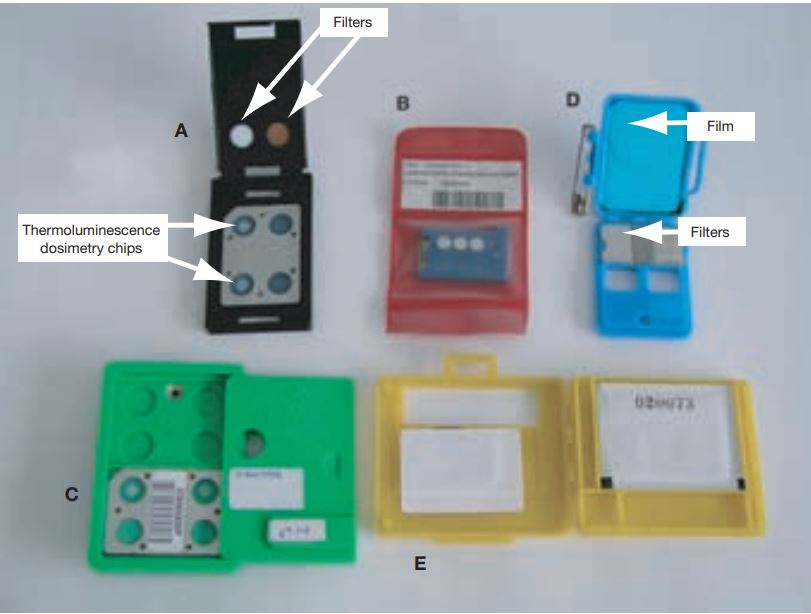
\includegraphics[width=0.5\textwidth]{Imagens/dosimetrosDeTorax.JPG}
		}%
		\caption{Dosímetros pessoais: exemplos de dosímetros de termoluminescência (A, B, C) e crachás de filme (D, E).}
		\label{fig:dosimetrosDeTorax}
	\end{figure}

	O objetivo principal do filme badge é detectar e caracterizar o tipo e a energia da radiação ionizante recebida por um indivíduo. Ele é utilizado para monitorar a exposição individual à radiação e fornece informações importantes sobre o tipo e a energia das partículas ionizantes que atingem o filme. Com base nas características dos padrões de exposição registrados no filme, é possível identificar a natureza da radiação e avaliar sua energia.

	Para fótons com energias acima de 100 keV, geralmente um único filtro é suficiente para a detecção adequada no filme badge. No entanto, para fótons de energia mais baixa, é necessário utilizar um sistema de filtros múltiplos. Isso ocorre porque a resposta do filme fotográfico não é uniforme em toda a faixa de energia dos fótons e pode variar significativamente em função da energia. Portanto, o uso de filtros múltiplos ajuda a melhorar a resposta do filme em relação a diferentes energias de fótons, permitindo uma caracterização mais precisa da radiação recebida.

	O filme badge não possui uma equivalência direta com o tecido humano em termos de resposta à radiação. Por isso, é necessário utilizar um sistema de filtros para uniformizar a resposta do filme em relação à energia, principalmente para fótons de energia mais baixa. Esse sistema de filtros é projetado para ajustar a resposta do filme badge e aproximá-la daquela que seria obtida com um material equivalente ao tecido humano. Dessa forma, é possível obter uma resposta mais representativa da dose de radiação que seria recebida pelos tecidos do corpo humano em uma exposição similar.

	\begin{exemplo}[Principais Características:]
		\begin{itemize}
			\item As doses cumulativas de radiação beta (b), raios-X (X), gama (g) e nêutrons térmicos são avaliadas pela medição das densidades ópticas (DOs) do filme sob diferentes filtros. Os resultados são então comparados com filmes de calibração que foram expostos a doses conhecidas de tipos de radiação bem definidos.
			\item O filme também pode ser utilizado como um monitor para nêutrons térmicos. Uma janela de cádmio é utilizada para absorver nêutrons térmicos, e a radiação gama resultante faz com que o filme escureça abaixo dessa janela, indicando a dose de nêutrons.
			\item Emulsões de track nuclear são utilizadas para monitorar nêutrons rápidos. Quando os nêutrons interagem com núcleos de hidrogênio na emulsão e no material circundante, prótons de recuo são produzidos por meio de colisões elásticas. Esses prótons criam uma imagem latente, resultando no escurecimento do filme ao longo de suas trilhas após o processamento.
			\item Os filmes são suscetíveis a efeitos adversos de vários agentes externos, como calor, líquidos e umidade excessiva. A imagem latente em filmes não revelados desvanece-se ao longo do tempo, limitando o período viável de uso a três meses em condições ideais.
		\end{itemize}
	\end{exemplo}

\subsection*{Porta TLDs}

	Um badge de dosimetria por termoluminescência é composto por um suporte de plástico que contém um conjunto de chips de dosímetro termoluminescente (TLD), juntamente com filtros apropriados. Esses chips de TLD são feitos de materiais específicos que exibem propriedades termoluminescentes, ou seja, emitem luz quando aquecidos após serem irradiados. O crachá é projetado para ser usado por indivíduos expostos à radiação ionizante, permitindo a medição das doses recebidas.

	Existem diferentes materiais de dosimetria por termoluminescência, também conhecidos como fósforos, que são comumente utilizados. Alguns exemplos desses materiais incluem \ce{LiF}:\ce{Ti},\ce{M} (Fluoreto Lítio dopado  com Titânio e Magnésio), \ce{CaSO4}:\ce{Dy} (Sulfato de Cálcio dopado com Disprósio) e \ce{CaF2}:\ce{Mn} (Fluoreto de Cálcio dopado com Manganês). Esses materiais têm a capacidade de armazenar a energia da radiação recebida e liberá-la na forma de luz quando aquecidos.

	O dosímetro de termoluminescência registra as doses de radiação provenientes de partículas beta, raios-X e raios gama. Para avaliar essas doses, a saída do dosímetro é medida usando diferentes filtros. Os filtros são usados para discriminar a contribuição específica de cada tipo de radiação na dose total registrada. Os resultados obtidos são então comparados com curvas de calibração estabelecidas para o badge de calibração. O badge de calibração é exposto a doses conhecidas de radiação em condições bem definidas, servindo como uma referência confiável para a medição de dose. Ao comparar os resultados do dosímetro com as curvas de calibração, é possível determinar com precisão a dose de radiação recebida pelo usuário do badge.

	\begin{exemplo}[Principais Características:]
		\begin{itemize}
			\item Badges que utilizam materiais de dosimetria por termoluminescência com alto número atômico (Z) não são equivalentes a tecido e, assim como filmes, requerem filtros para alinhar sua resposta de energia com a do tecido. Por outro lado, badges que utilizam materiais de dosimetria por termoluminescência com baixo número atômico (Z) não necessitam de sistemas de filtros complexos.
			\item O sinal de termoluminescência nos badges sofre desvanecimento (\textit{``fading''}), mas geralmente é menos significativo do que nos filmes.
			\item Badges projetados para monitoramento de partículas beta geralmente possuem um limiar relativamente alto (por volta de 50 keV) devido ao detector e à espessura de seu revestimento.
			\item Dosímetros de termoluminescência (TLDs) são convenientes para monitorar doses em partes específicas do corpo, como os olhos, braço ou punho, ou dedos, usando tipos especializados de dosímetros, incluindo dosímetros de extremidade.
			\item Diversas técnicas têm sido empregadas para o monitoramento de nêutrons, incluindo o uso do corpo como moderador para termalizar nêutrons (semelhante a dosímetros de albedo) ou o uso de \ce{LiF} enriquecido com \ce{^6Li} para aumentar a sensibilidade a nêutrons térmicos por meio da reação (n, $\alpha$) de nêutrons térmicos em \ce{^6Li}.
		\end{itemize}
	\end{exemplo}

\subsection*{Sistemas OLS}


	A luminescência opticamente estimulada (OSL) é uma técnica disponível comercialmente para a medição de doses pessoais de radiação ionizante. Os dosímetros luminescentes estimulados opticamente utilizam uma fina camada de óxido de alumínio (Al2O3:C) como material sensível à radiação.

	Durante o processo de análise, o óxido de alumínio é estimulado com frequências selecionadas de luz laser. Esse estímulo faz com que os elétrons armazenados nos centros de armadilha no óxido de alumínio sejam liberados, resultando em uma luminescência proporcional à exposição à radiação recebida. A intensidade da luminescência gerada é medida e usada para determinar a dose de radiação a que o dosímetro foi exposto.

	Os dosímetros OSL oferecem vantagens significativas, como alta sensibilidade, ampla faixa de dose linear, capacidade de armazenar informações de dose a longo prazo e resistência à radiação residual. Esses sistemas são amplamente utilizados para monitoramento individual de radiação em ambientes de trabalho onde há exposição a radiação ionizante.


	\begin{exemplo}[Principais Características:]
		\begin{itemize}
			\item Os distintivos disponíveis comercialmente são pacotes autônomos que vêm pré-carregados, incorporando uma tira de óxido de alumínio (\ce{Al2O3}) dentro de um pacote de filtro selado termicamente. Padrões especiais de filtro fornecem informações qualitativas sobre as condições de exposição.
			\item Os dosímetros luminescentes estimulados opticamente são altamente sensíveis. Por exemplo, o sistema Luxel pode ser usado com uma precisão de ±10 mSv e uma faixa de detecção de até 10 mSv. Essa alta sensibilidade os torna particularmente adequados para monitoramento individual em ambientes de baixa radiação. Os dosímetros podem ser utilizados em uma ampla faixa de doses de até 10 Sv e em feixes de fótons que variam de 5 keV a 40 MeV.
			\item Os dosímetros podem ser reanalisados várias vezes sem perder a sensibilidade e podem ser usados por até um ano.
		\end{itemize}
	\end{exemplo}

\bibliography{ref.bib}
\end{document}